% RLJ main.tex Version 2026.1

\documentclass[10pt]{article} % For LaTeX2e

%%%%%%%%%%%%%%%%%%%%%%%%%%%%%%%%%%%%%%%%%%%%%%%%%%%%%%%%%%%%%%%%
% AUTHOR: Select ONE option:
%      [accepted]{rlj} --> for camera ready (after peer review, if accepted)
%      {rlj}           --> for submission
%      [preprint]{rlj} --> to de-anonymize and remove references to RLJ/RLC
%%%%%%%%%%%%%%%%%%%%%%%%%%%%%%%%%%%%%%%%%%%%%%%%%%%%%%%%%%%%%%%%
% \usepackage{rlj}           % Should be uncommented for submission
%\usepackage[accepted]{rlj} % Should be uncommented for the camera-ready
\usepackage[preprint]{rlj} % Should be uncommented for preprint versions

%%%%%%%%%%%%%%%%%%%%%%%%%%%%%%%%%%%%%%%%%%%%%%%%%%%%%%%%%%%%%%%%
% WARNING: The following packages are already included in the
%          rlj.sty style file:
%
%  1. fancyhdr  - For controlling header/footers
%  2. natbib    - For formatting the bibliography
%  3. enumitem  - To customize the appearance of lists
%  4. fontenc (with option [T1]) - Allows for proper hyphenation and accents
%  5. times     - Times new roman font
%  6. ragged2e  - Used to justify text
%  7. tcolorbox - Used to create boxes on cover page
%  8. hyperref  - Configures hyperlinks throughout (e.g., links to references)
%  9. xcolor    - Used to define custom colors for links and boxes
%  10. amsmath  - Not used, but conflicts with lineno, so we include (and patch) it for authors
%  11. etoolbox - Included in the amsmath + lineno patch
%  12. lineno   - For adding line numbers when in submission
%
% You do not need to include them again in your main.tex.
% Including them again may lead to conflicts or compilation errors.
% Additionally, avoid loading packages that might conflict with these.
%%%%%%%%%%%%%%%%%%%%%%%%%%%%%%%%%%%%%%%%%%%%%%%%%%%%%%%%%%%%%%%%

%%%%%%%%%%%%%%%%%%%%%%%%%%%%%%%%%%%%%%%%%%%%%%%%%%%%%%%%%%%%%%%%
% Recommended (but not required) packages
%%%%%%%%%%%%%%%%%%%%%%%%%%%%%%%%%%%%%%%%%%%%%%%%%%%%%%%%%%%%%%%%
\usepackage{amssymb}            % Defines common symbols like \mathbb R
\usepackage{mathtools}          % Extends amsmath, providing common math tools
\usepackage{mathrsfs}           % Enables \mathscr, which can work in cases that \mathcal does not
%\mathtoolsset{showonlyrefs}     % Only number equations that are referenced (optional)
\usepackage{graphicx}           % For including images
\usepackage{subcaption}         % Allows for the use of subfigures and subcaptions
\usepackage[space]{grffile}     % For spaces in image names
\usepackage{url}                % For displaying URLs
\usepackage{lipsum}             % For placeholder text
\usepackage{amsthm}
\usepackage{cleveref}

\newtheorem{theorem}{Theorem}
\newtheorem{corollary}[theorem]{Corollary}
\newtheorem{proposition}[theorem]{Proposition}
\newtheorem{lemma}[theorem]{Lemma}
\usepackage{dsfont}
\usepackage{booktabs}
\usepackage{makecell}

\usepackage{color}

\usepackage{ifthen}
\newboolean{DisplayComments}
\setboolean{DisplayComments}{false}
% \setboolean{DisplayComments}{false}
\DeclareRobustCommand{\aj}[1]{\ifthenelse{\boolean{DisplayComments}}{{\color{red} (AJ: #1)}}{}}
\DeclareRobustCommand{\raj}[1]{\ifthenelse{\boolean{DisplayComments}}{{\color{blue} (Raj: #1)}}{}}
\DeclareRobustCommand{\yc}[1]{\ifthenelse{\boolean{DisplayComments}}{{\color{violet} (YC: #1)}}{}}
%%%%%%%%%%%%%%%%%%%%%%%%%%%%%%%%%%%%%%%%%%%%%%%%%%%%%%%%%%%%%%%%
% AUTHOR: Fill in the following meta-data
%%%%%%%%%%%%%%%%%%%%%%%%%%%%%%%%%%%%%%%%%%%%%%%%%%%%%%%%%%%%%%%%

% Enter the title of your paper:
\title{Safe RLHF Beyond Expectation: Stochastic Dominance for Universal Spectral Risk Control}

% The "running title" will be displayed in the header on every-other page.
% It is typically either the same as the title or a shorter version of the title.
% Enter your running title here:
\setrunningtitle{Safe RLHF Beyond Expectation}

% WARNING: Authors must not appear in the submitted version. They should be hidden
% as long as the rlj package is used without the [accepted] or [preprint] options.
% Non-anonymous submissions will be rejected without review.

% Enter the author names below.
% NOTE: Denote affiliations using superscripts as in the provided example.
% NOTE: Use \textscript{1,2,3} instead of $^{1,2,3}$.
%       - Failure to do so will cause affiliation superscripts to appear on the cover page for camera-ready and preprint versions.
\author{Yaswanth Chittepu\textsuperscript{1,$\dagger$}, Ativ Joshi\textsuperscript{1}, Rajarshi Bhattacharjee\textsuperscript{1}, Scott Niekum\textsuperscript{1}}

% NOTE: For camera-ready and preprint versions, the cover page includes author names but not affiliations.
% It automatically removes the superscripts for affiliations.
% If the automatic process breaks (e.g., if an author name should include a superscript), you can manually define the author string to appear on the cover page by uncommenting the following line.
%\coverPageAuthor{Marlos C. Machado, Philip S. Thomas, Lorem Ipsum}

% Author emails, which can be clustered if they have shared endings as in this example
\emails{\{ychittepu, atjoshi, rbhattacharj, sniekum\}@umass.edu}

% Author affiliations, in the order the occur
% The inclusion of state/province, etc. is optional.
% The inclusion of multiple affiliations is optional.
%   - List multiple affiliations with comma-separated numbers as in the example.
\affiliations{
  $^{1}$\textbf{University of Massachusetts Amherst}\\
  % $^{2}$\textbf{Alberta Machine Intelligence Institute (Amii)}\\
  % $^{3}$\textbf{CIFAR AI Chair}\\
  % $^{4}$\textbf{Manning College of Information and Computer Sciences, University of Massachusetts}
  % % The following two lines are optional and can be commented out
  % \par % If including additional comments like below, use \par to add some whitespace.
  % $^\dagger$ Additional comments can be added like this, e.g., indicating equal contribution
}

% \contribution{
%   % Contribution
%   Provide a succinct but precise list of the contribution(s) of the paper. Use contextual notes to avoid implications of contributions more significant than intended and to clarify and situate the contribution relative to prior work (see the examples below). If there is no additional context, enter ``None''. Try to keep each contribution to a single sentence, although multiple sentences are allowed when necessary. If using complete sentences, include punctuation. If using a single sentence fragment, you may omit the concluding period. A single contribution can be sufficient, and there is no limit on the number of contributions. Submissions will be judged mostly on the contributions claimed on their cover pages and the evidence provided to support them. Major contributions should not be claimed in the main text if they do not appear on the cover page. Overclaiming can lead to a submission being rejected, so it is important to have well-scoped contribution statements on the cover page.
% }
% {
%   % Caveat:
%   None
% }

% \contribution{
%   % Contribution
%   The submission template for submissions to RLJ/RLC 2026
% }
% {
%   % Caveat:
%   Built from previous RLC/RLJ, ICLR, and TMLR submission templates
% }

% \contribution{
%   % Contribution
%   \textit{{[}Example of one contribution and corresponding contextual note for the paper ``Policy gradient methods for reinforcement learning with function approximation'' \citep{Sutton2000}.]}\\ This paper presents an expression for the policy gradient when using function approximation to represent the action-value function.
% }
% {
%   % Context:
%   Prior work established expressions for the policy gradient without function approximation \citep{Williams1992}.
% }

\contribution{
  % Contribution
  We introduce Risk-sensitive Alignment via Dominance (RAD), a Safe RLHF objective that constrains the first-order stochastic dominance (FSD) of the learned policy’s cost distribution relative to a reference policy, rather than constraining only expected cost.
}
{
  % Context:
  Prior Safe RLHF \citep{dai2023safe} and HC-RLHF \citep{chittepu2025reinforcement} formulations impose scalar expected-cost or high-confidence expected-cost constraints, while we position RAD as bringing stochastic-dominance control into the safe-RLHF framework for policy-induced cost distributions.
}

\contribution{
  % Contribution
  We give a practical optimization procedure for this dominance objective by using an asymmetric quantile-gap surrogate, a nonparametric empirical quantile-particle representation of policy-induced cost distributions, and an entropically regularized optimal-transport formulation that yields a differentiable REINFORCE-style policy-gradient estimator.
}
{
  % Context:
  While the OT view of the FSD surrogate and Sinkhorn-based regularization have been explored \citep{melnyk2024distributional}, we adapt them to the sample-based Safe RLHF setting together with the resulting gradient estimator for optimizing the dominance-constrained objective.
}

\contribution{
  % Contribution
  We introduce quantile-weighted FSD constraints and show that they provide universal control over a broad class of Spectral Risk Measures (SRMs), enabling tunable risk sensitivity.
}
{
  % Context:
SRMs \citep{acerbi2002spectral} form a broad class of coherent \citep{artzner1999coherent}, law-invariant risk functionals that aggregate quantile costs using a weighted spectrum over
confidence levels.
}

\contribution{
  % Contribution
  Empirically, we show that RAD improves the harmlessness of model responses over baselines (Safe-RLHF, SFT) and generalizes better to out-of-distribution harmlessness evaluations, while maintaining competitive helpfulness relative to Safe-RLHF \citep{dai2023safe}.
}
{
  % Context:
We use the BeaverTails dataset \citep{ji2023beavertailsimprovedsafetyalignment} 
following \citet{dai2023safe}, and evaluate the helpfulness and harmlessness of RAD, Safe-RLHF, and SFT models, on its test split. We additionally evaluate out-of-distribution harmlessness on HarmBench 
\citep{mazeika2024harmbenchstandardizedevaluationframework}.
}





% Include a list of keywords for the topic of the paper:
\keywords{Reinforcement Learning from Human Feedback (RLHF), Safety, Alignment, Stochastic Dominance, Optimal Transport, Spectral Risk Measures} % Your keywords

% Define the summary that appears on the cover page.
\summary{

Safe RLHF typically enforces safety through expected cost constraints, but the expectation captures only a single statistic of the cost distribution and fails to account for distributional uncertainty, particularly under heavy tails or rare catastrophic events. We proposes Risk-sensitive Alignment via Dominance (RAD), a safe alignment framework that replaces expected-cost constraints with first-order stochastic dominance (FSD) constraints on the full cost distribution relative to a reference policy, implemented through an entropically regularized optimal transport objective. Furthermore, we introduce quantile-weighted dominance constraints and show that they provide universal control over a broad class of Spectral Risk Measures, enabling tunable risk sensitivity.

% The summary appears on the cover page. Although it can be identical to the abstract, it does not have to be. One might choose to omit the stated contributions in the Summary, given that they will be stated in the box below. The original abstract may also be extended to two paragraphs. The authors should ensure that the contents of the cover page fit entirely on a single page. The cover page does \textbf{not} count towards the 8--12 page limit.

  % \lipsum[1]
}

%%%%%%%%%%%%%%%%%%%%%%%%%%%%%%%%%%%%%%%%%%%%%%%%%%%%%%%%%%%%%%%%
%% Begin document, create title and abstract
%%%%%%%%%%%%%%%%%%%%%%%%%%%%%%%%%%%%%%%%%%%%%%%%%%%%%%%%%%%%%%%%
\begin{document}

\makeCover  % Create the cover page
\maketitle  % Make the title section

\begin{abstract}

  Safe Reinforcement Learning from Human Feedback (RLHF) typically enforces safety through expected cost constraints, but the expectation captures only a single statistic of the cost distribution and fails to account for distributional uncertainty, particularly under heavy tails or rare catastrophic events. This limitation is problematic when robustness and risk sensitivity are critical. Stochastic dominance offers a principled alternative by comparing entire cost distributions rather than just their averages, enabling direct control over tail risks and potential out-of-distribution failures that expectation-based constraints may overlook. In this work, we propose Risk-sensitive Alignment via Dominance (RAD), a novel alignment framework that replaces scalar expected cost constraints with First-Order Stochastic Dominance (FSD) constraints. We operationalize this constraint by comparing the target policy's cost distribution to that of a reference policy within an Optimal Transport (OT) framework, using entropic regularization and Sinkhorn iterations to obtain a differentiable and computationally efficient objective for stable end-to-end optimization. Furthermore, we introduce quantile-weighted FSD constraints and show that weighted FSD universally controls a broad class of Spectral Risk Measures (SRMs), so that improvements under weighted dominance imply guaranteed improvements in the corresponding spectral risk. This provides a principled mechanism for tuning a model's risk profile via the quantile weighting function. Empirical results demonstrate that RAD improves harmlessness over baselines while remaining competitive in helpfulness, and exhibits greater robustness on out-of-distribution harmlessness evaluations.
  
  % of model responses yields policies that are more robust to safety violations while maintaining competitive reward performance relative to expectation-based baselines.
  % Empirical results demonstrate that weighted FSD alignment enables a controllable safety-reward trade-off, with several spectral configurations achieving simultaneous improvements in both safety and reward, compared to expectation-based baselines.
  

  %  Safe Reinforcement Learning from Human Feedback (RLHF) typically enforces safety through expected cost constraints. But, the expectation provides only a single statistic of the distribution and fails to capture uncertainty in the distribution, particularly in the presence of heavy tails or rare but catastrophic events. This limitation is especially problematic when robustness and risk sensitivity are critical. (Break this sentence up)By contrast, stochastic dominance offers a principled framework for capturing distributional uncertainty by comparing the entire cost distribution rather than just its average, better accounting for high-variance tail risks and potential out-of-distribution failures, that expectation-based constraints may overlook.
  % (Connect these sentences) In this work, we propose a novel alignment framework that replaces scalar expected cost constraints with First-Order Stochastic Dominance (FSD) constraints.  We formulate this constraint by comparing the cost distribution of the target policy against a reference policy's cost distribution within an Optimal Transport (OT) framework. Specifically, we leverage Sinkhorn iterations to provide a differentiable and efficient approximation of the gradient of the FSD constraint with respect to policy parameters, enabling stable and efficient end-to-end policy optimization. Furthermore, we demonstrate that by applying non-uniform weighting schemes over cost quantiles, our framework can represent a broad class of constaints on Spectral Risk Measures. This allows practitioners to tune a model's risk profile simply by adjusting the weighting function. Our approach provides a unified optimization framework for safe alignment across diverse risk profiles. Empirical evaluations suggest that FSD-constrained alignment yields models that are more robust to safety violations while maintaining competitive reward performance compared to standard baselines.
\end{abstract}

\section{Introduction}
\label{sec: introduction}
% \textcolor{red}{JUST ADDING A SKETCH. FILL THIS OUT. MAKE THIS FLOW BETTER, MORE COHERENT, AND ADD CITATIONS WHEREVER NEEDED.}

% Talk about LLMs being used in real world and these include settings where safety is critical. This necessitates LLMs that produce helpful responses that are safe (i.e no toxicity, misinformation)
Large Language Models (LLMs) are now used across a wide range of applications, so it is important that their outputs are helpful, reliable, and safe. This need is especially acute in high-stakes domains such as legal reasoning (\cite{katz2024gpt}), medical consultation (\cite{yang2022large,moor2023foundation}), and educational support (\cite{kasneci2023chatgpt,kung2023performance}), where harmful generations—including toxicity and misinformation—can have serious consequences (\cite{gehman2020realtoxicityprompts,weidinger2021ethical,ganguli2022red}).

Broadly, we want LLMs to be \textit{helpful} and aligned with human preferences, while being \textit{harmless}, i.e. prevent toxic outputs. But there may be scenarios when users may request assistance with potentially harmful activities (\cite{Bai2022ConstitutionalAH,glaese2022improving}). Thus, \emph{harmlessness} and \emph{helpfulness} can conflict. The standard technique for aligning LLMs with human preferences, Reinforcement Learning from Human Feedback (RLHF), typically optimizes a single reward model for both objectives (\cite{Ouyang2022TrainingLM,bai2022traininghelpfulharmlessassistant}), or heuristically mixes separate reward models (\cite{glaese2022improving,touvron2023llama,mu2024rule}). This creates trade-offs: stronger harmlessness can lead to refusals, while stronger helpfulness can increase unsafe outputs (\cite{bai2022traininghelpfulharmlessassistant}). Recent work addresses this by decoupling preference data and enforcing harmlessness as a constraint, an approach known as Safe RLHF (\cite{dai2023safe}). However, Safe RLHF typically typically constrains the expected cost of a policy, providing no guarantees on worst-case or tail outcomes.  This is inadequate in high-stakes deployments where tail risk is critical — such as code generation \cite{pearce2021asleepkeyboardassessingsecurity} and open-ended dialogue where rare but severe harms including toxic generations and private data leakage can impact users
\citep{perez2022redteaminglanguagemodels, gehman2020realtoxicityprompts}.

%To overcome this limitation, Safe RLHF modifies both the reward modeling and reinforcement learning phases, explicitly introducing a safety constraint to minimize harmfulness while preserving helpfulness.

% Helpfullness and Safety can conflict with each other. Talk about seperating these objectives, framing the problem as a constrained optimization problem, which was used in Safe-RLHF.

%However, , yet standard
% FSD is a principled approach to compare distributions and better handles uncertainity. FSD is partial ordering, hence making it harder to optimize

\yc{Also, I changes the flow of the old paragraph, and incorporated scott's comments. Lmk if this seems good or not}\raj{we already talk about expected cost contraints above. Moved the first line to the pargarph above since it is more expressive.}
%Safe alignment methods typically constrain the \textit{expected} cost of a policy, providing no guarantees on worst-case or tail outcomes.
Thus, we argue that a stronger notion of constraining the cost of the policy is needed: the cost distribution of the learned policy should be \emph{stochastically smaller} than that of the reference policy, not merely cheaper on average. \raj{added a linbe which explains what it means to be stcoshstically smaller} This means that the learned policy should assign less probability to high-cost outcomes across the distribution, not just reduce the mean cost. This motivates \textbf{Risk-sensitive Alignment via Dominance (RAD)}, which enforces a First-Order Stochastic Dominance (FSD) constraint on the cost distribution of the learned policy relative to a reference policy.

A key insight of RAD is that by reweighting quantiles of the FSD objective, we recover Spectral Risk Measures (SRMs) — a family of risk measures defined as a weighted integral of the cost quantiles,
$\int w(q) Q_X(q) dq$, where $Q_X(q)$ is the quantile function of the cost distribution and the weighting function $w(q)$ allows
practitioners to express diverse risk preferences over the cost distribution. For instance, concentrating weight on upper quantiles recovers tail-sensitive measures such as CVaR, while uniform weighting recovers the mean — both expressible within our unified framework. This is practically valuable: a medical deployment may demand near-zero tolerance for harmful outputs, while a general assistant
may tolerate a more permissive tradeoff, and both are accommodated by choosing $w$ appropriately.

Optimizing FSD constraints directly is challenging, so we relax them to an asymmetric FSD-violation surrogate that aggregates positive quantile gaps (see \Cref{eq:fsd_loss}). We interpret stochastic
dominance through Optimal Transport (OT) and derive an efficient REINFORCE-style policy gradient using Sinkhorn iterations, yielding an end-to-end differentiable approach. Empirically, RAD yields models that are more robust to safety violations while achieving competitive helpfulness across multiple spectral risk measures relative to Safe RLHF.
% and under several spectral risk measures achieve simultaneous improvements in both safety and helpfulness. 
\yc{IS this ok, given the results?}\raj{modified a bit}

% In this work, we propose \textbf{Risk-sensitive Alignment via Dominance (RAD)}, which performs safe alignment by enforcing a First-Order Stochastic Dominance (FSD) constraint that makes the learned policy's costs stochastically smaller than a reference policy's costs.
% Optimizing FSD constraints is challenging, so we relax them to an asymmetric FSD-violation surrogate that aggregates positive quantile gaps (see \Cref{eq:fsd_loss}).
% We interpret stochastic dominance through Optimal Transport (OT) and propose an efficient REINFORCE-style algorithm. Using Sinkhorn iterations, we derive a policy-gradient expression for the FSD objective, yielding an end-to-end differentiable approach to optimize FSD-based constraints or objectives. We further show that reweighting quantiles recovers Spectral Risk Measures (SRMs): imposing FSD constraints with a given weighting yields, at convergence, a reduction in the corresponding SRM whenever reverse violations vanish.
% % imposing FSD loss constraints with a given weighting guarantees, at convergence, a reduction in the corresponding SRM relative to the reference policy's cost distribution.
% This lets practitioners tune the risk profile by choosing the weighting function, providing a unified approach to safe alignment. Experimentally, SARD yields models that are more robust to safety violations while achieving competitive helpfulness compared to expected-constraint methods such as Safe-RLHF.

% \aj{Need to add a para about how the paper is structured and one or two lines about the experiments and observations.}

\aj{verify}
Our main contributions are: (i) we formulate safe alignment as a dominance-constrained objective over the full cost distribution rather than only its expectation, (ii) we derive a RAD policy-gradient estimator using entropic OT and Sinkhorn iterations, making optimization of the objective end-to-end differentiable, (iii) we connect quantile reweighting in our framework to SRMs, enabling controllable risk-sensitive alignment profiles, and (iv) through extensive experiments, we show that RAD improves robustness to safety violations while maintaining competitive helpfulness relative to expected cost based baselines. \aj{extra} The rest of the paper is organized as follows: \Cref{sec: background} reviews Safe RLHF, stochastic dominance, and SRMs; \Cref{sec: method} presents RAD and its optimization procedure; \Cref{sec: results} reports empirical evaluations safety--helpfulness trade-offs; and \Cref{sec: relatedwork,sec: conclusion} is related work and conclusion respectively.
\aj{Can write one or two lines highlighting the conclusion of experiments.}\raj{changed second point. Replacing unregularized with regaularized OT is not really an original contribution and pretty standard. But we show how to estimate the gradients which could be a new contribution} \yc{Add experimental conclusions as a point in our contribution} \raj{added experimental contributional.}


\section{Background and Problem Setting}
\label{sec: background}
% \aj{Perhaps we can change the title to something like "Background and Model" as we are also introducing how we model the loss etc.}

% \aj{One important thing missing that's missing is the non-parametric representation of the distributions. Right now, it is pushed into the proof of theorem $1$ in the supplementary material \cref{sec:sard-pol-grad}}
\subsection{Reinforcement Learning from Human Feedback (RLHF)}

The most popular method of aligning LLMs with human preferences is Reinforcement Learning from Human Feedback (RLHF). The standard RLHF pipeline consists of three phases as described in \cite{Christiano2017DeepRL,Ouyang2022TrainingLM}. The first phase is a supervised fine-tuning (SFT) phase where the outputs of a pre-trained model are aligned with human responses. This is followed by a reward modeling phase, where a reward model is trained using human preferences and finally, a reinforcement learning phase where the model is optimized using the learned reward function. Formally, let  $x \sim D_x$  denote prompts and  $y \sim \pi_\theta(\cdot \mid x)$  denote model responses. SFT produces a reference policy  $\pi_{\mathrm{sft}}$, and we set  $\pi_{\mathrm{ref}} := \pi_{\mathrm{sft}}$  unless stated otherwise. A reward model  $r_\phi(x,y)$  is learned from preference comparisons using the Bradley-Terry model \citep{bradley1952rank}. Details are standard and deferred to \Cref{supp:RLHF}.

RLHF then optimizes a KL-regularized objective to prevent reward overoptimization and preserve language quality \citep{Ouyang2022TrainingLM,stiennon2022learningsummarizehumanfeedback,Gao2022ScalingLF,Rafailov2024ScalingLF}:
\begin{align}
  \max_\theta\;\mathbb{E}_{x \sim D_x,\, y \sim \pi_\theta(\cdot\mid x)}\!\big[r_\phi(x,y)\big]\;-\;\beta\,D_{\mathrm{KL}}\!\Big(\pi_\theta(\cdot\mid x)\,\Vert\,\pi_{\mathrm{ref}}(\cdot\mid x)\Big),
\end{align}
equivalently maximizing the KL-regularized reward  $\tilde r(x,y)=r_\phi(x,y)-\beta\log\frac{\pi_\theta(y\mid x)}{\pi_{\mathrm{ref}}(y\mid x)}$. In practice, this objective is optimized with PPO/GRPO/REINFORCE-style methods \citep{williams1992simple,ahmadian2024basicsrevisitingreinforcestyle,shao2024deepseekmathpushinglimitsmathematical,schulman2017proximalpolicyoptimizationalgorithms}.

%%%%%%%%%%%%%%%%%%%%%%%%%%%%%%%%%%%%%%%%%%%%%%%%%%%%%%%%%%%

\subsection{Safe RLHF}
Standard RLHF optimizes a single reward function learned from human preferences, which may be inadequate when attempting to balance competing goals such as \emph{helpfulness} and \emph{harmlessness}. In contrast, Safe RLHF \citep{dai2023safe} separates helpfulness and harmlessness by learning (i) a reward model  $r_\phi(x,y)$, (parameterized by $\phi$ and for input prompt $x$ and model output $y$)  from helpfulness preferences and (ii) a cost model  $c_\psi(x,y)$, (parameterized by $\psi$)  from harmfulness preferences, and then solving the expected-cost constrained RL problem:
\begin{align}
  \max_\theta\;\mathbb{E}\big[r_\phi(x,y)\big] - \beta D_{\mathrm{KL}}(\pi_\theta\Vert \pi_{\mathrm{ref}}) \quad\text{s.t.}\quad \mathbb{E}\big[c_\psi(x,y)\big]\le \tau.
  \label{eq:safe-rlhf-obj}
  % \vspace{-0.3in}f
\end{align}

High-confidence variants like HC-RLHF \citep{chittepu2025reinforcement} replace the expectation constraint with a probabilistic guarantee using the Seldonian framework \citep{thomas2019preventing}.

% Standard RLHF optimizes a single reward function, derived from human preferences, which can be insufficient when trying to balance objectives that may conflict with each other, such as helpfulness and harmlessness. To address this, Safe-RLHF \citep{dai2023safe} imposes an explicit harmfulness constraint, optimizing model responses to improve helpfulness while reducing harmfulness.

% Safe-RLHF collects two preference annotations for each prompt: one indicating which response is more helpful and one indicating which is more harmful. The helpfulness preferences are used to train a reward model, while the harmfulness labels are used to train a cost model. The reward model $r_{\phi}$ and the cost model $c_{\psi}$ are trained using the standard Bradley–Terry objective in Equation~\ref{eq:bt_rm_loss}. Safe-RLHF then solves the following constrained optimization problem to increase the helpfulness of model responses while reducing harmfulness.

% \begin{align}
%   \max_{\theta} \text{\space} &\mathbb{E}_{x \sim \mathcal D_x, y \sim \pi_{\theta}(\cdot \vert x)}[r_{\phi}(x,y)] - \beta \mathbb{D}_\mathrm{KL}\big(\pi_{\theta}(.\vert x) \vert\vert \pi_\mathrm{ref}(. \vert x)\big) \label{eq: obj_safe_rlhf}\\
%   %
%   \text{s.t.} \quad & \mathbb{E}_{x \sim \mathcal D_x, y \sim \pi_{\theta}(\cdot \vert x)}[c_{\psi}(x,y)] \leq \tau. \label{eq: safety constraint}
% \end{align}

% \aj{Can we move this to a related works section?}

% Even though Safe-RLHF reduces the harmfulness of model responses, it does not provide any guarantees on the safety of the resulting model. High Confidence-RLHF (HC-RLHF) \citep{chittepu2025reinforcement} incorporates the Seldonian framework \citep{thomas2019preventing}, modifying the constraint to be a probabilistic upper bound on the expected cost of model responses. It also uses a simpler REINFORCE \citep{ahmadian2024basicsrevisitingreinforcestyle} style algorithm, significantly improving both the helpfulness and harmlessness of model responses compared to Safe-RLHF.

\subsection{First-Order Stochastic Dominance}
\label{sec:fosd}

\aj{cite for FSD} \raj{incorporated Scott's suggestion about describing our approach more accuartely.}
The expected cost constraint in Safe RLFH often proves inadequate in settings where controlling the tail risk is crucial. A more robust method for controlling tail risk is ensuring that the learned policy's cost is stochastically smaller than the cost of the reference policy i.e. less probability must be assigned by the learned policy to high cost outcomes compared to the reference policy. We now describe how we do this formally. Let $F_{X}$ and $Q_{X}$ denote the Cumulative Distribution Function (CDF) and the Quantile Function (Inverse CDF) of a random variable $X$.
For real-valued random variables  $X,Y$, $X$ is said to have first-order stochastic dominance (FSD) on $Y$  (denoted by $X \succeq_{\mathrm{FSD}} Y$)  iff  $F_X(r)\le F_Y(r)$  for all  $r$ \citep{dai2023learning}. Equivalently, we also have $Q_X(q)\ge Q_Y(q)$  for all  $q\in[0,1]$.

%We do this by imposing a first-order stochastic dominance (FSD) constraint. In this section, we decribe the FSD objective formally.

% Since FSD is only a partial order, we use the standard asymmetric violation functional
% \begin{align}
%   \mathcal{L}_{\mathrm{FSD}}(X,Y):=\int_0^1\big(Q_Y(q)-Q_X(q)\big)_+\,dq,
% \end{align}
% which satisfies  $\mathcal{L}_{\mathrm{FSD}}(X,Y)=0$  whenever  $X\succeq_{\mathrm{FSD}} Y$  and relates to Wasserstein-1 via $\mathcal{L}_{\mathrm{FSD}}(X,Y)+\mathcal{L}_{\mathrm{FSD}}(Y,X)=W_1(X,Y)$.
% Moreover, this functional admits an OT characterization with asymmetric convex cost  $c(x,y)=(y-x)_+$  \citep{melnyk2024distributional,Santambrogio2015OptimalTF}, which is what enables our differentiable implementation.

%%%%%%%%%%

% Let $F_{X}$ and $Q_{X}$ denote the Cumulative Distribution Function (CDF) and the Quantile Function (Inverse CDF) of a random variable $X$. We consider the setting when all the random variables are scalar valued, i.e $X, Y \in \mathbb{R}$. A random variable $X$ is said to dominate another random variable $Y$, in First-Order Stochastic Dominance (FSD) sense, $X \succeq_{\text{FSD}} Y$ if

% \begin{equation}
%   F_{X}(r) \leq F_{Y}(r) \quad \forall r \in \mathbb{R}
% \end{equation}

% This can also be expressed in an alternate form, that uses the Quantile function (Inverse CDF) instead of the CDF

% \begin{equation}
%   Q_{X}(q) \geq Q_{Y}(q) \quad \forall q \in [0,1]
% \end{equation}

% One drawback of FSD is that it only imposes a partial ordering over distributions of real valued random variables i.e there can exist two random variables where neither of them dominate the other. This makes it harder to optimize the FSD between two random variables. Hence, we relax the FSD criterion to instead be a loss that measure the extent to which a random variable $X$ \underline{\emph{is dominated by}} another Random Variable $Y$. The FSD loss can be expressed as follows %\aj{since this is a new formulation, should this be in the background section?}

% \begin{equation}
%   \mathcal{L}_\mathrm{FSD}(X,Y) := \int_{0}^{1} \big(Q_{Y}(q) - Q_{X}(q)\big)_{+} dq
%   \label{eq:fsd-loss}
% \end{equation}

% where $(x)_{+} = \max(x,0)$  denotes the ReLU function. This loss measures how much a Random variable $X$ is dominated by $Y$.

Practically, a drawback of FSD is that it only imposes a partial ordering over distributions, so two random variables may be incomparable in terms of FSD. Hence, we relax the definition to an objective that measures the extent to which $X$ falls below $Y$ across quantiles:
\begin{equation}
  \mathcal{L}_{\mathrm{FSD}}(X,Y)
  := \int_{0}^{1} \big(Q_Y(q)-Q_X(q)\big)_+\, dq,
  \label{eq:fsd_loss}
\end{equation}
where $(x)_+=\max(x,0)$ denotes the ReLU function. Note that for two random variables $X$ and $Y$ with different distributions, an FSD objective of $0$ implies that X dominates Y, i.e.  $X \succeq_{\mathrm{FSD}} Y$. More generally,  $\mathcal{L}_{\mathrm{FSD}}(X,Y)$  aggregates the positive quantile gaps  $(Q_Y(q)-Q_X(q))_+$  and therefore quantifies the extent to which  $X$  fails to dominate  $Y$ or $Y$ dominates $X$; it does not by itself certify  $Y\succeq_{\mathrm{FSD}}X$.

In our case, we set $X$ to be the cost distribution $C_{\pi_{\theta}}$ under our learned policy $\Pi_{\theta}$ and $Y$ to be the cost distribution $C_{\pi_{\mathrm{ref}}}$ under the reference policy $\Pi_{\mathrm{ref}}$. Thus, $\mathcal{L}_{\mathrm{FSD}}(C_{\pi_{\theta}},C_{\pi_{\mathrm{ref}}})$ quantifies by how much the cost distribution of the reference policy dominates the cost distribution of the learned policy\footnote{Note that $\mathcal{L}_{\mathrm{FSD}}(X,Y)$ is not a distance because it is not symmetric and can be zero even when $X$ and $Y$ have different distributions. Also $\mathcal{L}_\mathrm{FSD}(X,Y) + \mathcal{L}_\mathrm{FSD}(Y,X) = \mathcal{W}_{1}(X,Y)$ where $\mathcal{W}_{1}(X,Y)$ is the 1-Wassertsein distance }.
% A higher loss implies greater domination by Y on X, but need \underline{\emph{NOT}} imply that Y dominates X.

% \aj{extra: move to footnote}  The following equation relates the FSD objectives $\mathcal{L}_\mathrm{FSD}(X,Y)$ and $\mathcal{L}_\mathrm{FSD}(Y,X)$ to the 1-Wassertsein distance $\mathcal{W}_{1}(X,Y)$:
% \begin{equation}
%   \mathcal{L}_\mathrm{FSD}(X,Y) + \mathcal{L}_\mathrm{FSD}(Y,X) = \mathcal{W}_{1}(X,Y)
% \end{equation}
%In particular, $\mathcal{L}_{\mathrm{FSD}}(X, Y) = 0$ whenever $X \succeq_{\mathrm{FSD}} Y$, even if $X$ and $Y$ are not identically distributed.
%where $\mathcal{W}_{1}(X,Y)$ is the 1-Wasserstein distance.
% between the distributions of X and Y, and can be expressed as \citep{peyre2020computationaloptimaltransport}:
% \begin{equation}
%   \mathcal{W}_{1}(X,Y) = \int_{0}^{1} \big\vert Q_{Y}(q) - Q_{X}(q) \big\vert dq
% \end{equation}

% Using the results from \citet{Santambrogio2015OptimalTF} (Theorem 2.9 and Proposition 2.17) or \citet{melnyk2024distributional} (Theorem 1), the FSD loss can be framed as an optimal transport problem. Specifically,
% \begin{align}
%   \mathcal{L}_\mathrm{FSD}(X,Y) = \mathrm{OT}_c(X,Y)
% \end{align}
% for the asymmetric convex cost function $c(x,y)=(y-x)_+$. We restate the relevant theorem in \Cref{supp:FSD} for completeness.

% As we describe in the next section, FSD is closely related to the optimal transport problem.
%We use \eqref{eq:quantile_particles}--\eqref{eq:empirical_measure} throughout for optimization and gradients.

%With this representation, integrals over quantile levels are approximated by Riemann sums on the fixed grid
%$\{\alpha_i\}_{i=1}^N$.

\subsection{Optimal Transport}\label{subsec:ot}

% Optimal Transport (OT) provides a principled way to compare distributions by optimizing over couplings \citep{peyre2020computationaloptimaltransport}. In our use, OT is primarily a computational tool for building a differentiable surrogate of dominance constraints. We rely on the entropically regularized OT objective \citep{cuturi2013sinkhorn}, which replaces a linear program with a strictly convex problem:
% \begin{align}
%   \mathrm{OT}^{\lambda}_{c}(\mu,\nu) := \min_{P\in \Pi(\mu,\nu)}\;\langle P,C\rangle - \lambda H(P),
% \end{align}
% where  $C_{ij}=c(x_i,y_j)$  and  $H(P)=-\sum_{ij}P_{ij}\log P_{ij}$. The optimizer admits the Sinkhorn scaling form  $P^\star=\mathrm{diag}(u)\,K\,\mathrm{diag}(v)$  with  $K_{ij}=\exp(-C_{ij}/\lambda)$, computable via Sinkhorn iterations \citep{cuturi2013sinkhorn,peyre2020computationaloptimaltransport}. We place full OT/Sinkhorn details in \Cref{supp:ot}, since we only need the fact that the resulting objective is smooth and differentiable w.r.t. its inputs.

%%%%%%%%%%%%%%%%
Optimal transport \citep{peyre2020computationaloptimaltransport} studies the problem of optimally transforming a distribution $\mu$ into another distribution $\nu$ under a cost function
$c(x,y) : \mathcal{X} \times \mathcal{Y} \to \mathbb{R}_+$, which represents the cost of moving a unit mass from $x$ to $y$.

Let $\mu = \sum_{i=1}^N a_i\,\delta_{x_i}$ and $\nu = \sum_{j=1}^M b_j\,\delta_{y_j}$ be two empirical (atomic) distributions on $\mathbb{R}^{d}$, where $x_i, y_j \in \mathbb{R}^d$ are support points (“particles”), $a \in \Delta^N$ and $b \in \Delta^M$ are nonnegative weights summing to 1 ($\Delta^N$ denotes the $N$-dimensional probability simplex), and $\delta_z$ is a Dirac mass at $z$.

A \emph{transport plan} (a.k.a. coupling) from $\mu$ to $\nu$ is a nonnegative matrix $P \in \mathbb{R}_+^{N \times M}$ whose row and column sums match the marginals. Intuitively, $P_{ij}$ represents the amount of probability mass moved from $x_i$ to $y_j$. The set of admissible couplings can be represented as:
\begin{equation}
  \Pi(\mu,\nu) := \Bigl\{ P \in \mathbb{R}_+^{N \times M} \;:\; P \mathbf{1}_M = a, \;\; P^\top \mathbf{1}_N = b \Bigr\}.
  \label{eq:transport-plans}
\end{equation}

Given a ground cost function $c:\mathbb{R}^d \times \mathbb{R}^d \to \mathbb{R}_+$, define the cost matrix $C_{ij} = c(x_i, y_j)$. The \textbf{Kantorovich optimal transport problem} \citep{peyre2020computationaloptimaltransport} between $\mu$ and $\nu$ is
\begin{equation}
  \mathrm{OT}_c(\mu, \nu) := \min_{P \in \Pi(\mu,\nu)} \langle P, C \rangle
  = \min_{P \in \Pi(\mu,\nu)} \sum_{i=1}^N \sum_{j=1}^M P_{ij}\, c(x_i, y_j).
  \label{eq:kantorovich-ot}
\end{equation}

The above objective function is a linear programming problem. Solving this directly is computationally expensive. Hence, to approximate the solution, an entropically regularized OT objective is usually preferred \citep{cuturi2013sinkhorn}, which replaces the linear program with a strictly convex problem:
\begin{align}
  \mathrm{OT}^{\chi}_{c}(\mu,\nu) := \min_{P\in \Pi(\mu,\nu)}\;\langle P,C\rangle - \chi H(P),\label{eq:ot-unreg}
\end{align}
where $H(P)=-\sum_{ij}P_{ij}\log P_{ij}$ and $\chi$ is the regularization parameter. This optimization problem is smooth and has a unique minimizer, which is computable via Sinkhorn iterations \citep{cuturi2013sinkhorn,peyre2020computationaloptimaltransport}. We explain the full details of regularized OT and the Sinkhorn Algorithm in \Cref{supp:ot}.

\yc{Also mention how we are different from Melynk, that they have a direct parametrization of reward with policy, where we only have access to samples and use empirical approximation of distribution i.e our approiach is more general where rewards are generated stochastically and we cannot use the reparameterization trick to express them directly as function of policy parameters}

% \aj{Since the FSD loss is written in terms of integral, should we also write the OT problem in its Lebesgue integral form?}
% \raj{Since we wroking with discrete (empirical) distributions, maybe we can keep this as is and, in section 2.4,define eq 6 as a sum?  }
%\aj{extra} Since we work with (empirical) discrete measures, we use the discrete formulations (see \Cref{eq:fsd_sum_approx}).
%\Cref{eq:kantorovich-ot,eq:ot-unreg}.
%Integrals appear only in the population quantile definitions in \Cref{sec:fosd}, which we approximate by Riemann sums in practice (see \Cref{eq:fsd_sum_approx}).
% \aj{Are the following two equations necessary?}
% A common choice for the cost function is the $p$-norm of the difference between points:
% \begin{equation}
%   c(x_i, y_j) = \| x_i - y_j \|_p^p, \quad p \ge 1,
% \end{equation}
% which leads to the definition of the \emph{$p$-Wasserstein distance} between $\mu$ and $\nu$, denoted as $\mathcal{W}_{p}(\mu, \nu)$.
% \begin{equation}
%   \mathcal{W}_p(\mu, \nu) := \Big(\min_{P \in \Pi(a,b)} \sum_{i=1}^N \sum_{j=1}^M P_{ij}\, \|x_i - y_j\|_p^p.\Big)^{\frac{1}{p}}
%   \label{eq:wasserstein-distance}
% \end{equation}

% \subsubsection{Entropic Regularization and the Sinkhorn Algorithm}

% The optimal transport problem can be solved using linear programming \citep{dantzig2016linear, dvurechensky2018computational}, but this can be computationally expensive when the number of particles is large. Instead, we use entropic regularization, which adds an entropy term to the objective and allows for efficient optimization using the Sinkhorn algorithm \citep{cuturi2013sinkhorn}. Let us define an parameterized empirical distribution $\mu_{\theta}$, where the locations of the particles could be the parameters themselves, and a reference distribution $\nu$. Specifically, we define the entropic regularized OT problem as
% \begin{equation}
%   \mathrm{OT}_{c}^\lambda(\mu_\theta,\nu_{\mathrm{ref}}) \;=\; \min_{P\in\Pi(a,b)}\;\langle P,C\rangle - \lambda H(P), \quad H(P)\;=\;-\sum_{i,j} P_{ij}\log P_{ij},
%   \label{eq:entropic-ot}
% \end{equation}

% for  $\lambda>0$ and a cost matrix $C$. This problem is strictly convex in  $P$  and has a unique minimizer  $P^\star$. More importantly, it can be solved efficiently using the Sinkhorn algorithm \citep{cuturi2013sinkhorn}, which iteratively updates scaling vectors to enforce the marginal constraints. The resulting transport plan  $P^\star$  can then be used to compute the optimal transport objective and its gradient with respect to the policy parameters  $\theta$.

% Define the Gibbs kernel
% \begin{equation}K_{ij} \;=\; e^{-C_{ij}/\lambda}.
%   \label{eq:gibbs-kernel}
% \end{equation}The optimal transport plan can be expressed in closed form as
% \begin{equation}P^\star \;=\; \mathrm{diag}(u) K \mathrm{diag}(v),
%   \label{eq:optimal-plan}
% \end{equation}where  $u \in \mathbb{R}^N$, $v\in\mathbb{R}^M$  are scaling vectors that can be computed using the Sinkhorn iterations
% \begin{equation}u^{(t+1)} \;=\; \frac{a}{Kv^{(t)}}, \qquad v^{(t+1)} \;=\; \frac{b}{K^\top u^{(t+1)}},
%   \label{eq:sinkhorn-iterations}
% \end{equation}starting from some positive initialization (e.g.  $u^{(0)}=v^{(0)}=\mathbf 1$). The iterations are guaranteed to converge to the unique optimal plan  $P^\star$  that satisfies the marginal constraints \citep{peyre2020computationaloptimaltransport, cuturi2013sinkhorn}. Once we have  $P^\star$, we can compute the FSD loss as
% \begin{equation}
%   \mathcal{L}_{\mathrm{FSD}}^\lambda(\mu_\theta,\nu_{\mathrm{ref}}) \;=\; \langle P^\star,C\rangle - \lambda H(P^\star).
%   \label{eq:fsd-loss-sinkhorn}
% \end{equation}

% Because the algorithm consists only of a fixed number of matrix-vector multiplications and divisions, gradients can be propagated through the iterations using automatic differentiation in frameworks like PyTorch \citep{NEURIPS2019_9015} or JAX \citep{jax2018github}, making the Sinkhorn algorithm end to end differentiable.

\paragraph{Relation to FSD.}
We now describe how our FSD objective relates to the optimal transport objective. Using the results from \citet{Santambrogio2015OptimalTF} (Theorem 2.9 and Proposition 2.17) or \citet{melnyk2024distributional} (Theorem 1), for any two distributions $X$ and $Y$, the FSD objective can be framed as an optimal transport problem. Specifically,
\begin{align}\label{eq:otl}
  \mathcal{L}_\mathrm{FSD}(X,Y) = \mathrm{OT}_c(X,Y)
\end{align}
for the asymmetric convex cost function $c(x,y)=(y-x)_+$. We restate the relevant theorem in \Cref{supp:FSD} for completeness. We note that while \cite{melnyk2024distributional} also aims to do alignment via optimal transport, they apply stochastic dominance directly to reward distributions which are derived from a specific parametric form. On the other hand, we only have access to the cost distribution of a policy (independent from the reward distribution) which we access only through sampling. Hence, our framework is more general as we do not assume any specific parametric form. 

% The FSD loss can be framed as an optimal transport problem under an asymmetric convex cost:
% \begin{equation}
%   \mathcal{L}_{\mathrm{FSD}}(X,Y) = \mathrm{OT}_c(\mu_X,\mu_Y),
%   \qquad
%   c(x,y)=(y-x)_+,
%   \label{eq:fsd_ot}
% \end{equation}
% where $\mu_X,\mu_Y$ are the laws of $X,Y$ (see Section C for a formal statement).

% The computation of the FSD loss can be framed as an optimal transport problem, using the results from \citet{Santambrogio2015OptimalTF} (Theorem 2.9 and Proposition 2.17) or \citet{melnyk2024distributional} (Theorem 1). We restate the theorem below.

% \begin{theorem}[from \citet{melnyk2024distributional}]
%   \label{thm:fsd_as_ot}
%   Let $h : \mathbb{R} \to \mathbb{R}_{+}$ be a convex function, and let
%   $X$ and $Y$ be real-valued random variables with probability measures
%   $\mu_X$ and $\mu_Y$, respectively. Denote by
%   $Q_X, Q_Y : [0,1] \to \mathbb{R}$ their (left-continuous) quantile functions.

%   Then,
%   \begin{equation}
%     \int_0^1 h\big(Q_X(q) - Q_Y(q)\big)\, dq
%     =
%     \min_{\gamma \in \Pi(\mu_X,\mu_Y)}
%     \int_{\mathbb{R}^2} h(x-y)\, d\gamma(x,y),
%   \end{equation}
%   where $\Pi(\mu_X,\mu_Y)$ denotes the set of all couplings
%   (joint probability measures) on $\mathbb{R}^2$ with marginals
%   $\mu_X$ and $\mu_Y$. Moreover, if $h$ is strictly convex, the minimizing transport plan $\gamma^\star$ is unique.
% \end{theorem}

% \begin{corollary}[FSD as asymmetric optimal transport]
%   \label{cor:fsd_as_ot}
%   Let $X,Y$ be real-valued random variables with measures
%   $\mu_X$ and $\mu_Y$, and define the FSD loss
%   \[
%     \mathcal{L}_{\mathrm{FSD}}(X,Y)
%     :=
%     \int_0^1 \big(Q_Y(q) - Q_X(q)\big)_+ \, dq.
%   \]
%   Then
%   \[
%     \mathcal{L}_{\mathrm{FSD}}(X,Y)
%     =
%     \min_{\gamma \in \Pi(\mu_X,\mu_Y)}
%     \int_{\mathbb{R}^2} (y-x)_+ \, d\gamma(x,y),
%   \]
%   that is, the FSD loss coincides with the optimal transport cost under the
%   asymmetric convex cost function $c(x,y)=(y-x)_+$.
% \end{corollary}

% Note that the regularized loss  $\mathcal{L}_{\mathrm{FSD}}^\lambda$  is a smooth approximation of the original FSD loss  $\mathcal{L}_{\mathrm{FSD}}$, and as  $\lambda\to0$, we have  $\mathcal{L}_{\mathrm{FSD}}^\lambda \to \mathcal{L}_{\mathrm{FSD}}$. In practice, we can choose a small value of  $\lambda$  to balance approximation accuracy and computational efficiency.

\subsection{Spectral Risk Measures}

Spectral risk measures (SRMs) \citep{acerbi2002spectral} form a broad class of coherent \citep{artzner1999coherent}, law-invariant risk
functionals that aggregate quantile costs using a weighted spectrum over
confidence levels. They provide a flexible way to emphasize parts of the cost distribution (especially the tail) according to application-specific risk tolerance, rather than relying only on the mean. SRMs are widely used in fields like financial risk management and actuarial science to quantify and control exposure to adverse outcomes (\citet{dowd2008spectral,adam2008spectral}). Let $X$ be a real-valued random variable with quantile function
$Q_X : [0,1] \to \mathbb{R}$. A \emph{spectral risk measure} is defined as
\begin{equation}
  \rho_\phi(X)
  =
  \int_0^1 Q_X(q)\,\phi(q)\,dq,
\end{equation}
where $\phi : [0,1] \to \mathbb{R}_+$ is a non-negative, non-decreasing
weighting function satisfying
$\int_0^1 \phi(q)\,dq = 1.$
The function $\phi$ is referred to as the \emph{risk spectrum} and encodes
risk sensitivity across quantiles. Larger weights at higher quantiles emphasize higher
tail costs, while uniform weighting recovers the expectation.
% A canonical example is Conditional Value-at-Risk at level $\alpha$, which corresponds to a step-function spectrum $\phi(q)=\frac{1}{1-\alpha}\mathbf{1}_{[\alpha,1]}(q)$:
% \begin{equation}
%   \mathrm{CVaR}_\alpha(X)
%   =
%   \frac{1}{1-\alpha}
%   \int_\alpha^1 Q_X(q)\,dq.
% \end{equation}
% \aj{Extra}
% SRMs satisfy coherence (monotonicity, subadditivity,
% positive homogeneity, and translation invariance)
% \citep{artzner1999coherent}, and admit the Kusuoka representation,
% which characterizes them as mixtures of Conditional Value-at-Risk (CVaR)
% levels \citep{kusuoka2001law}.

% In Section~\ref{subsec:srm}, we show that how we can use a suitable weighted version of the FSD objective~\eqref{eq:fsd_loss} to represent a broad set of SRMs.
% that places zero weight on quantiles less than $\alpha$ and $\frac{1}{1-\alpha}$ weight everywhere else.
% \begin{equation}
%   \phi(q)
%   =
%   \frac{1}{1-\alpha}\mathbf{1}_{[\alpha,1]}(q).
% \end{equation}

% Thus, SRMs generalize CVaR by allowing structured or smooth weighting over quantiles, providing a flexible mechanism for encoding tail sensitivity in distributional optimization settings.


\section{Risk-sensitive Alignment via Dominance}
\label{sec: method}

% \section{Safe Alignment via Risk and Dominance}

We now present our safe alignment formulation -- \emph{Risk-sensitive Alignment via Dominance  (RAD)}. Standard Safe RLHF constrains the \emph{expected} cost, which controls only a single moment of the cost distribution.
% RAD instead enforces a \emph{distributional} safety constraint using first-order stochastic dominance (FSD), implemented via the asymmetric FSD cost $\mathcal{L}_{\mathrm{FSD}}$ (Eq.~\eqref{eq:fsd_loss}).
RAD instead enforces a \emph{distributional} safety constraint using first-order stochastic dominance (FSD). We first introduce FSD as a principled way to ensure the learned policy's cost distribution is
stochastically smaller than a reference,
% \yc{stochastically smaller again}
implemented via the asymmetric FSD surrogate $\mathcal{L}_{\mathrm{FSD}}$ (Eq.~\eqref{eq:fsd_loss}). We then show that reweighting quantiles of this surrogate recovers
Spectral Risk Measures (SRMs), yielding a unified framework in which the choice of weighting function $w(q)$ controls the risk profile of the learned policy.
Recall that our reward model is denoted by $r_{\phi}(x,y)$ and our cost model is denoted by $c_{\psi}(x,y)$ for input $x$ and ouptut $y$ and for learned parameters $\phi$ and $\psi$. For a policy $\pi$, let $C_\pi := c_\psi(x,y)$ denote the random variable of costs induced by sampling
$x\sim\mathcal{D}_x$ and $y\sim\pi(\cdot\mid x)$. Thus, we solve:
\begin{align}
  \max_\theta \quad & \mathbb{E}_{x\sim D_x,\,y\sim\pi_\theta(\cdot\mid x)}\!\Big[r_\phi(x,y)\Big]
  - \beta\,D_{\mathrm{KL}}\!\big(\pi_\theta(\cdot\mid x)\,\|\,\pi_{\mathrm{ref}}(\cdot\mid x)\big), \label{eq:sard_primal_obj}\\
  \text{s.t.}\quad & \mathcal{L}_{\mathrm{FSD}}\!\big(C_{\pi_\theta},\,C_{\pi_{\mathrm{ref}}}\big)\;\ge\;\kappa. \label{eq:sard_primal_constr}
\end{align}
Constraint~\eqref{eq:sard_primal_constr} encourages \emph{uniform} improvement across quantiles: since
$\mathcal{L}_{\mathrm{FSD}}(C_{\pi_\theta},\,C_{\pi_{\mathrm{ref}}})=\int_0^1 (Q_{C_{\pi_{\mathrm{ref}}}}(q)-Q_{C_{\pi_\theta}}(q))_+\,dq$,
larger values of $\mathcal{L}_{\mathrm{FSD}}\!\big(C_{\pi_\theta},C_{\pi_{\mathrm{ref}}}\big)$ correspond to larger positive gaps $Q_{C_{\pi_{\mathrm{ref}}}}(q)-Q_{C_{\pi_\theta}}(q)$ over $q\in[0,1]$.
Equivalently, it encourages $C_{\pi_{\mathrm{ref}}}\succeq_{\mathrm{FSD}} C_{\pi_\theta}$, i.e., the learned policy has stochastically smaller costs. %\yc{stochasticall smaller again}.
% pushes the learned-policy cost quantiles downward relative to the reference across the distribution, not only in expectation.

To optimize our objective, we first absorb the KL term into the reward by defining the KL-regularized reward
$\tilde r(x,y)= r_\phi(x,y)-\beta\log \frac{\pi_\theta(y\mid x)}{\pi_{\mathrm{ref}}(y\mid x)}$ as done in \cite{dai2023safe},
and then use Dual Ascent \citep{gallier2019fundamentals} to optimize the Lagrangian relaxation of \eqref{eq:sard_primal_obj}--\eqref{eq:sard_primal_constr}:
\begin{equation}
  \max_\theta\min_{\lambda\ge 0}\;\underbrace{
    \mathbb{E}_{x\sim D_x,\,y\sim\pi_\theta(\cdot\mid x)}\!\Big[\tilde r(x,y)\Big]
  +\lambda\Big(\mathcal{L}_{\mathrm{FSD}}\!\big(C_{\pi_\theta},C_{\pi_{\mathrm{ref}}}\big)-\kappa\Big)}_{L(\theta,\lambda)}. \label{eq:sard_dual}
\end{equation}

\paragraph{Non-parametric (quantile-particle) representation of policy-induced cost distributions.}
\label{subsec:nonparam}
We now describe how we represent the cost distributions for our policies.
For a policy $\pi$, rather than assuming a parametric family for the cost distribution $C_\pi$, we use a non-parametric empirical approximation
via particles in the \emph{quantile space}. Fix quantile levels $\alpha_1,\dots,\alpha_N\in(0,1)$ and define the corresponding
cost-quantile particles:
\begin{equation}
  q_i(\pi) := Q_{C_\pi}(\alpha_i),\qquad i=1,\dots,N,
  \label{eq:quantile_particles}
\end{equation}
which we assume are ordered so that $q_1(\pi)\le \cdots \le q_N(\pi)$.
We approximate the cost distribution by the empirical measure:
\begin{equation}
  \hat\mu_\pi := \frac{1}{N}\sum_{i=1}^N \delta_{q_i(\pi)}.
  \label{eq:empirical_measure}
\end{equation}
In practice, $\hat\mu_\pi$ is obtained by sampling generations from $\pi$, evaluating their costs via $c_\psi$,
and computing empirical quantiles from the resulting samples; these quantiles serve as the particles defining the discrete
representation. Let $\hat{\mu}_{\pi_{\theta}}$ and $\hat{\mu}_{\pi_{\mathrm{ref}}}$ be the empirical measures for the cost distrivutions corresponding to policies $\pi_{\theta}$ and $\pi_{\mathrm{ref}}$ respctively. Then, the FSD objective is approximated as $\mathcal{L}_{\mathrm{FSD}}\!\big(C_{\pi_\theta},\,C_{\pi_{\mathrm{ref}}}\big) \approx \mathcal{L}_{\mathrm{FSD}}\!\big(\hat{\mu}_{\pi_{\theta}},\,\hat{\mu}_{\pi_{\mathrm{ref}}}\big)$. %\yc{commented out the equation below. Lmk if this is needed}\aj{works}
% The FSD objective between two such policy-induced cost distributions $C_{\pi_\theta}$ and $C_{\pi_{\mathrm{ref}}}$ is given by:
% \begin{equation}
%   \mathcal{L}_{\mathrm{FSD}}\!\big(C_{\pi_\theta},\,C_{\pi_{\mathrm{ref}}}\big) \approx \mathcal{L}_{\mathrm{FSD}}\!\big(\hat{\mu}_{\pi_{\theta}},\,\hat{\mu}_{\pi_{\mathrm{ref}}}\big)
%   \;=\;
%   \frac{1}{N}\sum_{i=1}^N \big(q_i(\pi_{\mathrm{ref}})-q_i(\pi_\theta)\big)_+.
%   \label{eq:fsd_sum_approx}
% \end{equation}
\paragraph{Computing the RAD policy gradients.}
% \yc{removed the part about non-differentiability, as subgradients do work. Can be a reviewer headache. Just mention the challenge is the gradient of the FSD term wrt theta}
% The main technical challenge for computing the gradients of the RAD policy is differentiating the FSD term in~\eqref{eq:fsd_sum_approx} with respect to the quantiles efficiently. The FSD objective is not smooth with respect to particle positions. It is also non-differentiable and small perturbations in particle locations can induce discontinuous changes in the gradient.
The main technical challenge for computing the gradients of the RAD policy is differentiating the FSD term with respect to the policy parameters $\theta$.
To compute the gradients of the FSD objective effectively, first note that it can be interpreted as an optimal transport problem between the two cost distributions as described in~\eqref{eq:otl}. On adding entropic regularizion, the resulting optimization problem in~\eqref{eq:ot-unreg} is strictly convex and differentiable. Moreover, the entropic regularized optimal problem has smooth gradients and the unique minimizer of the objective can be computed efficiently using Sinkhorn iterations. Hence, we replace the FSD objective with the entropic regularzied FSD objective $\mathcal{L}^{\chi}_{\mathrm{FSD}}$ where $\chi$ is the regularization parameter (as in~\eqref{eq:ot-unreg}) \yc{$\beta$ already used in KL regularized rewards. Change this to $\chi$} \aj{We are also using the superscript for the weighted version of $\mathcal{L}$}. We next state the resulting policy-gradient estimator; the full derivation and implementation details are deferred to Supplementary Material ~\ref{app:sard_pg_derivation}.

\begin{theorem}[RAD policy-gradient estimator]\label{thm:sard_pg}
  Fix $\lambda\ge 0$ and define the dual objective $L(\theta,\lambda)$ by \eqref{eq:sard_dual}.
  Let $\alpha_1,\dots,\alpha_N\in(0,1)$ be fixed quantile levels and let
  $q_i(\pi_\theta):=Q_{C_{\pi_\theta}}(\alpha_i)$ denote the corresponding cost-quantile values. Using the empirical quantile-particle approximation from \Cref{eq:empirical_measure},
  the gradient $\nabla_\theta L(\theta,\lambda)$ admits the REINFORCE-form estimator
  \begin{equation}
    \nabla_\theta L(\theta,\lambda)
    =
    \mathbb{E}_{x\sim D_x,\,y\sim\pi_\theta(\cdot\mid x)}
    \Bigg[
      \Bigg(\tilde r(x,y)+\lambda\sum_{i=1}^N
        \Big(-\frac{\partial \mathcal{L}^{\chi}_{\mathrm{FSD}}}{\partial q_i(\pi_\theta)}\Big)\,
        \mathbf{1}\!\big(c_\psi(x,y)\le q_i(\pi_\theta)\big)
      \Bigg)
      \nabla_\theta\log\pi_\theta(y\mid x)
    \Bigg]. \label{eq:sard_pg}
  \end{equation}
  Moreover, for the weighted dominance objective $\mathcal{L}^{w}_{\mathrm{FSD}}$ (see \Cref{eq:weighted-fsd-loss-dfn}),
  the same estimator holds with an additional factor $w(\alpha_i)$ multiplying the $i$th summand. %\aj{Weighted FSD loss hasn't been introduced yet}
\end{theorem}
% \aj{Is the following line correct? REINFORCE \citep{williams1992simple} with RLOO \citep{Kool2019Buy4R} and Dual Ascent \citep{gallier2019fundamentals} were mentioned in the previous draft.}
We optimize \eqref{eq:sard_dual} by alternating (i) ascent in $\theta$ using \eqref{eq:sard_pg} with REINFORCE \citep{williams1992simple} and variance-reduction scheme (RLOO) \citep{Kool2019Buy4R}, and (ii) Dual Ascent \citep{gallier2019fundamentals} in $\lambda$ to enforce the constraint.

% \aj{------------------------------}

% We now propose our approach: \underline{\textbf{Safe Alignment via Risk and Dominance (RAD)}}. Instead of enforcing a constraint on the expected costs of the model generations, which ignores tail risks, we propose a stochastic dominance constraint that ensures that the cost distribution of reference model generations dominates the cost distribution of the model generations. Stochastic Dominance offers a principled framework for capturing distributional uncertainity, unlike expected value constraints that only represent a snapshot/statistic of the cost ditribution. But, imposing a raw First-Order Stochastic Dominance (FSD) constraint makes the optimization harder, becuse FSD only imposes a partal ordering over distributions. Hence, we relax the FSD constraint to the metric $\mathcal{L}_{\mathrm{FSD}}$, proposed in Equation ~\ref{eq:fsd-loss}. The RAD objective is provided below:

% \begin{align}
%   \max_{\theta} \text{\space} &\mathbb{E}_{x \sim \mathcal D_x, y \sim \pi_{\theta}(\cdot \vert x)}[r_{\phi}(x,y)] - \beta \mathbb{D}_\mathrm{KL}\big(\pi_{\theta}(.\vert x) \vert\vert \pi_\mathrm{ref}(. \vert x)\big) \label{eq: sard-objective}\\
%   %
%   \text{s.t.} \quad & \mathcal{L}_{\mathrm{FSD}}(c_{\psi}(\pi_{\theta}), c_{\psi}(\pi_{\mathrm{ref}})) \geq \kappa. \label{eq: sard-constraint}
% \end{align}

% In the Constraint in Equation ~\ref{eq: sard-constraint}, $c_{\psi}(\pi_{\theta})$ and $c_{\psi}(\pi_{\mathrm{ref}})$ denote the random variables representing the distribution of costs of the model's and the reference model's generations respectively, for prompts $x \sim \mathcal{D}_{x}$. The constraint enforces that the cost distribution of the reference policy first-order stochastically dominates that of the learned policy by at least a value of $\kappa$. Operationally, this encourages the optimizer to identify a policy whose quantile costs are uniformly lower than those of the reference policy across quantile levels, with a gap of at least $\kappa$. In other words, improvements are promoted not merely in expectation but throughout the distribution, including high-cost regions. Notably, the present formulation weights all quantile levels equally, assigning uniform importance across the entire cost spectrum.

% Henceforth, we subsume the KL penalty into the rewards, using the KL regularized reward $\Tilde{r}(x,y) = r_{\phi}(x,y) - \beta \log \frac{\pi_{\theta}(y \vert x)}{\pi_{\mathrm{ref}}(y \vert x)}$ as the objective we want to maximize, subject to a FSD constraint that ensures the cost distribution of the reference policy's generations dominates that of our policy's generations by a value of atleast $\kappa$.

% To solve (\ref{eq: sard-objective}), we use lagrangian relaxation \citep{boyd2004convex} and covert the convert the constrained primal problem into a dual problem, with a lagrangian multiplier $\lambda \geq 0$, that we optimize using Dual Ascent \citep{gallier2019fundamentals}.

% \begin{align}\label{eq:RAD-dual}
%   \max_{\theta} \min_{\lambda \geq 0} \text{\space} &\mathbb{E}_{x \sim \mathcal D_x, y \sim \pi_{\theta}(.\vert x)}\Big[\Tilde{r}(x,y)\Big] + \lambda \Big(\mathcal{L}_{\mathrm{FSD}}(c_{\psi}(\pi_{\theta}), c_{\psi}(\pi_{\mathrm{ref}})) - \kappa\Big).
% \end{align}

% To optimize the objective in Equation~\ref{eq:RAD-dual}, we require its gradient with respect to $\theta$. While the gradient of the reward term can be computed using standard policy gradient techniques, differentiating the FSD loss term is considerably more involved. In particular, evaluating this term entails either computing an intractable integral over quantile levels or solving an optimal transport problem, even for a single forward pass. We therefore derive an estimator for the policy gradient of the Dual RAD objective next.

% \aj{Add the policy gradient estimate as a thm here, and move the rest of the section to the appendix. Can give a brief sketch in 2-3 lines.}

\subsection{Universality of Weighted FSD for Controlling Spectral Risk Measures}\label{subsec:srm}

% \textcolor{red}{Scott: UNIFICATION IS NOT EMPHASIZED HERE AT ALL. MAYBE THIS IS NOT UNIFICATION, since FSD IS NOT AN SRM. UNIVERSALITY OF FSD FOR REASONING ABT SPECTRAL RISK MEASURES (something like this)}

We now describe how we can change the FSD objective to represesnt various spectral risk measures. The FSD objective in Equation~\ref{eq:fsd_loss} weights all quantiles equally.
However, in many applications, tail performance is of primary concern, and it may be desirable to emphasize higher quantiles more heavily than lower ones.
To accommodate this, we introduce a quantile-weighted FSD objective with a nonnegative weighting function $w(q)$:
\begin{equation}
  \mathcal{L}_{\mathrm{FSD}}^{w}(X,Y)
  =
  \int_{0}^{1} w(q) \big(Q_{Y}(q) - Q_{X}(q)\big)_{+} dq,
  \label{eq:weighted-fsd-loss-dfn}
\end{equation}
where $w(q) \ge 0$ for all $q \in [0,1]$ and $\int_0^1 w(q) dq = 1$. While $\mathcal{L}_{\mathrm{FSD}}^{w}(X,Y)$ is not itself a spectral risk measure (SRM), it admits a direct structural relationship to the entire class of SRMs.
Recall that a spectral risk measure associated with weight function $w$ is defined as
\(
  \rho_w(Z) := \int_0^1 Q_Z(q)\, w(q)\, dq.
\)
Note that we have the following relationship:
\begin{equation}
  \int_{0}^{1} w(q) \big(Q_{Y}(q) - Q_{X}(q)\big) dq
  =
  \rho_w(Y) - \rho_w(X).
\end{equation}

Thus, weighted quantile differences correspond exactly to differences in spectral risk measures.
The following proposition formally states that the weighted FSD violations provide a decomposition of spectral risk differences.

\begin{proposition}
  Let $w : (0,1) \to \mathbb{R}_{+}$ be any nonnegative weight function with $\int_0^1 w(q) dq = 1$, and define
  \(
    \rho_w(Z) := \int_0^1 Q_Z(q)\, w(q)\, dq .
  \)
  For two random variables $X$ and $Y$, define
  {\small
    \[
      \mathcal{L}_{\mathrm{FSD}}^{w}(X,Y)
      :=
      \int_0^1 \big(Q_Y(q) - Q_X(q)\big)_+\, w(q)\, dq,
      \quad
      \mathcal{L}_{\mathrm{FSD}}^{w}(Y,X)
      :=
      \int_0^1 \big(Q_X(q) - Q_Y(q)\big)_+\, w(q)\, dq.
    \]
  }
  Then,
  {\small
    \[
      \rho_w(Y) - \rho_w(X)
      =
      \mathcal{L}_{\mathrm{FSD}}^{w}(X,Y)
      -
      \mathcal{L}_{\mathrm{FSD}}^{w}(Y,X).
      \implies
      - \mathcal{L}_{\mathrm{FSD}}^{w}(Y,X)
      \;\le\;
      \rho_w(Y) - \rho_w(X)
      \;\le\;
      \mathcal{L}_{\mathrm{FSD}}^{w}(X,Y).
    \]
  }
\end{proposition}

This proposition shows that differences in \emph{any} spectral risk measure can be decomposed into two weighted FSD violations.
Thus, weighted FSD provides a universal dominance-based control mechanism for the entire class of spectral risk measures.
\begin{corollary}
  If $\mathcal{L}_{\mathrm{FSD}}^w(X,Y) \geq \kappa$ for some $\kappa > 0$, then
  \[
    \rho_w(Y) - \rho_w(X)
    =
    \mathcal{L}_{\mathrm{FSD}}^w(X,Y)
    -
    \mathcal{L}_{\mathrm{FSD}}^w(Y,X)
    \ge
    \kappa
    -
    \mathcal{L}_{\mathrm{FSD}}^w(Y,X).
  \]
  In particular, if $Y \succeq_{\mathrm{FSD}} X$ so that
  $\mathcal{L}_{\mathrm{FSD}}^w(Y,X) = 0$, then
  \(
    \rho_w(X)
    \le
    \rho_w(Y) - \kappa.
  \)
  \label{cor:srm-fsd-relation}
\end{corollary}
% where $\kappa>\mathcal{L}_{\mathrm{FSD}}^w(Y,X)$.
Note that when $\kappa>\mathcal{L}_{\mathrm{FSD}}^w(Y,X)$, enforcing $\mathcal{L}_{\mathrm{FSD}}^w(X,Y) \geq \kappa$ implies reduction in $\rho_w(X)$ w.r.t. $\rho_w(Y)$.
This corollary formalizes the universality property:
enforcing a lower bound on the weighted FSD violation guarantees improvement under the corresponding spectral risk measure, provided reverse violations vanish.

Substituting the cost distributions $X = C_{\pi_{\theta}}$ and
$Y = C_{\pi_{\mathrm{ref}}}$ into Corollary~\ref{cor:srm-fsd-relation}, enforcing
\[
  \mathcal{L}_{\mathrm{FSD}}^w(C_{\pi_{\theta}},C_{\pi_{\mathrm{ref}}}) \ge \kappa
  \implies
  \rho_w\!\left(C_{\pi_{\theta}}\right)
  \le
  \rho_w\!\left(C_{\pi_{\mathrm{ref}}}\right)
  -
  \kappa
  +
  \mathcal{L}_{\mathrm{FSD}}^w(C_{\pi_{\mathrm{ref}}},C_{\pi_{\theta}}).
\]

In particular, if
\( C_{\pi_{\mathrm{ref}}}\succeq_{\mathrm{FSD}} C_{\pi_{\theta}} \),
then \( \mathcal{L}_{\mathrm{FSD}}^w(C_{\pi_{\mathrm{ref}}},C_{\pi_{\theta}})=0 \), yielding the strict spectral risk improvement
\(
  \rho_w\!\left(C_{\pi_{\theta}}\right)
  \le
  \rho_w\!\left(C_{\pi_{\mathrm{ref}}}\right)
  -
  \kappa.
\)
In practice, as optimization proceeds under the weighted FSD constraint,
\( \mathcal{L}_{\mathrm{FSD}}^w(C_{\pi_{\theta}},C_{\pi_{\mathrm{ref}}}) \) increases while
\( \mathcal{L}_{\mathrm{FSD}}^w(C_{\pi_{\textrm
{ref}}},C_{\pi_{\theta}}) \) decreases, typically approaching zero near convergence.

Table~\ref{tab:spectral_weights} lists representative spectral risk measures and their associated quantile-weighting functions. Figure ~\ref{fig:srm-illustration} illustrates the spectral weighting function for different SRMs considered in Table~\ref{tab:spectral_weights}. For example, if $w(q)$ corresponds to $\mathrm{CVaR}_{\alpha}$, then enforcing
\(
  \mathcal{L}_{\mathrm{FSD}}^w(C_{\pi_{\theta}},C_{\pi_{\mathrm{ref}}}) \ge \kappa
\)
guarantees
\(
  \mathrm{CVaR}_{\alpha}\!\left(C_{\pi_{\theta}}\right)
  \le
  \mathrm{CVaR}_{\alpha}\!\left(C_{\pi_{\mathrm{ref}}}\right)
  -
  \kappa,
\)
whenever reverse violations vanish.
If $w(q)$ is uniform, corresponding to the unweighted FSD objective, then enforcing the FSD constraint guarantees that, at convergence,
\(
  \mathbb{E}[C_{\pi_{\theta}}]
  \le
  \mathbb{E}[C_{\pi_{\mathrm{ref}}}]
  -
  \kappa.
\)

\begin{table}[t]
  \centering
  \small
  % \begin{tabular}{l l}
  %   \hline
  %   \textbf{Risk Measure} & \textbf{Weight Function $w(q)$} \\
  %   \hline

  %   Mean & $1$\\[0.5em]

  %   Value-at-Risk (VaR$_\alpha$)
  %   &
  %   $\delta(q-\alpha)$
  %   \\[0.5em]

  %   Conditional Value-at-Risk (CVaR$_\alpha$)
  %   &
  %   $\frac{1}{1-\alpha}\mathbf{1}_{[\alpha,1]}(q)$
  %   \\[0.75em]

  %   Linear Spectral
  %   &
  %   $2q$
  %   \\[0.75em]

  %   Exponential Spectral
  %   &
  %   $\frac{\lambda e^{\lambda q}}{e^\lambda - 1}$
  %   \\[0.75em]

  %   Power Spectral
  %   &
  %   $(1+\lambda) q^\lambda$
  %   \\[0.75em]

  %   Wang Distortion
  %   &
  %   $\frac{\Phi(\Phi^{-1}(q)+\lambda)}
  %   {1-\Phi(\lambda)}$
  %   \\
  %   \hline
  % \end{tabular}
  {\footnotesize
    \begin{tabular}{l c c c c c c c}
      \hline
      \textbf{Risk} & \textbf{Mean} & \textbf{VaR$_\alpha$} & \textbf{CVaR$_\alpha$} & \textbf{Linear} & \textbf{Exponential} & \textbf{Power} & \textbf{Wang} \\
      \textbf{Measure}
      &
      & \textbf{}
      & \textbf{}
      & \textbf{Spectral}
      & \textbf{Spectral}
      & \textbf{Spectral}
      & \textbf{Distortion}
      \\
      \hline

      \textbf{$\mathbf{w(q)}$}
      & $1$
      & $\delta(q-\alpha)$
      & $\frac{1}{1-\alpha}\mathbf{1}_{[\alpha,1]}(q)$
      & $2q$
      & $\frac{\lambda e^{\lambda q}}{e^\lambda - 1}$
      & $(1+\lambda) q^\lambda$
      & $\frac{\Phi(\Phi^{-1}(q)+\lambda)}{1-\Phi(\lambda)}$
      \\
      \hline
    \end{tabular}
  }
  \caption{Examples of weight functions $w(q)$ that induce corresponding spectral risk measure constraints when used in $\mathcal{L}_{\mathrm{FSD}}^{w}$. $\lambda > 0$ denotes a risk aversion parameter and $\Phi$ in the Wang Distortion \citep{wang1996premium} risk measure denotes the CDF of a standard normal distribution.}
  \label{tab:spectral_weights}
\end{table}
Thus, though a weighted FSD is not a spectral risk measure by itself, it serves as a universal dominance-based control mechanism for the entire class of spectral risk measures.

% \subsection{Universality of weighted FSD for controlling spectral risk measures} The FSD loss in Equation~\ref{eq:fsd-loss} weights  all quantiles equally. But, in situations where tail risk performance is critical, it might be beneficial to impose a weighting over quantiles where higher quantiles have larger weight than lower quantiles. We now propose a quantile-weighted FSD loss that incorporates a quantile-dependent weighting function.

% \begin{equation}
%   \mathcal{L}_{\mathrm{FSD}}^{w}(X,Y) = \int_{0}^{1} w(q) \big(Q_{Y}(q) - Q_{X}(q)\big)_{+} dq
%   \label{eq:weighted-fsd-loss-dfn}
% \end{equation}

% We further add a constraint on the weighting function, such that $w(q) \geq 0, \,\forall q \in [0,1]$ and $\int_{0}^{1} w(q) dq = 1$.

% Now consider the weighted FSD loss integral without the ReLU function. From the defenition of Spectral Risk Measures (SRMs) ($\rho_{w})$, we can express the integral as follows.

% \begin{equation}
%   \int_{0}^{1} w(q) \big(Q_{Y}(q) - Q_{X}(q)\big) dq = \rho_{w}(Y) - \rho_{w}(X)
% \end{equation}

% \begin{proposition}
%   Let $w : (0,1) \to \mathbb{R}_{+}$ be any nonnegative weight function, and define the spectral risk measure
%   \[
%     \rho_w(Z) := \int_0^1 Q_Z(q)\, w(q)\, dq .
%   \]
%   For two random variables $X$ and $Y$, define
%   \[
%     \mathcal{L}_{\mathrm{FSD}}^{w}(X,Y) := \int_0^1 \big(Q_Y(q) - Q_X(q)\big)_+\, w(q)\, dq,
%   \]
%   \[
%     \mathcal{L}_{\mathrm{FSD}}^{w}(Y,X) := \int_0^1 \big(Q_X(q) - Q_Y(q)\big)_+\, w(q)\, dq.
%   \]
%   Then,
%   \[
%     \rho_w(Y) - \rho_w(X)
%     =
%     \mathcal{L}_{\mathrm{FSD}}^{w}(X,Y) - \mathcal{L}_{\mathrm{FSD}}^{w}(Y,X).
%   \]
%   Consequently, the following two-sided bound holds:
%   \[
%     - \mathcal{L}_{\mathrm{FSD}}^{w}(Y,X)
%     \;\le\;
%     \rho_w(Y) - \rho_w(X)
%     \;\le\;
%     \mathcal{L}_{\mathrm{FSD}}^{w}(X,Y).
%   \]
% \end{proposition}

% % \noindent
% % Thus, controlling the weighted FSD violation $L_w(X,Y)$ upper-bounds the increase in the corresponding spectral risk measure, while $R_w(X,Y)$ analogously controls decreases.

% \begin{corollary}
%   % Let
%   % \[
%   % \Delta(q) := Q_{\pi}(q) - Q_{\mathrm{ref}}(q),
%   % \]
%   % and let $w(q) \ge 0$ be a nonnegative weight function. Define
%   % \[
%   % L_w := \int_0^1 w(q)\, \max(\Delta(q),0)\, dq,
%   % \quad
%   % R_w := \int_0^1 w(q)\, \max(-\Delta(q),0)\, dq.
%   % \]
%   % Then,

%   If $\mathcal{L}_{\mathrm{FSD}}^w(X,Y) \geq \kappa$ for some $\kappa > 0$, then
%   \[
%     \rho_w(Y) - \rho_w(X)
%     =
%     \mathcal{L}_{\mathrm{FSD}}^w(X,Y) - \mathcal{L}_{\mathrm{FSD}}^w(Y,X)
%     \ge
%     \kappa - \mathcal{L}_{\mathrm{FSD}}^w(Y,X).
%   \]
%   which implies
%   \[
%     \rho_w(X)
%     \le
%     \rho_w(Y)
%     -
%     \kappa
%     +
%     \mathcal{L}_{\mathrm{FSD}}^w(Y,X).
%   \]
%   In particular, if $Y \succeq_{\text{FSD}} X$ i.e $\mathcal{L}_{\mathrm{FSD}}^w(Y,X) = 0$, then
%   \[
%     \rho_w(X)
%     \leq
%     \rho_w(Y) - \kappa
%   \]
%   \label{cor:srm-fsd-relation}
% \end{corollary}

% \textcolor{red}{Scott: UNIFICATION IS NOT EMPHASIZED HERE AT ALL. MAYBE THIS IS NOT UNIFICATION, since FSD IS NOT AN SRM. UNIVERSALITY OF FSD FOR REASONING ABT SPECTRAL RISK MEASURES (something like this)}

% \noindent
% Substituting $X = c_{\psi}(\pi_{\theta})$ and $Y = c_{\psi}(\pi_{\mathrm{ref}})$ into Corollary~\ref{cor:srm-fsd-relation}, enforcing
% \[
%   \mathcal{L}_{\mathrm{FSD}}^w(X,Y) \ge \kappa
% \]
% implies
% \[
%   \rho_w\!\left(c_{\psi}(\pi_{\theta})\right)
%   \le
%   \rho_w\!\left(c_{\psi}(\pi_{\mathrm{ref}})\right)
%   -
%   \kappa
%   +
%   \mathcal{L}_{\mathrm{FSD}}^w(Y,X).
% \]
% In particular, if
% \( c_{\psi}(\pi_{\mathrm{ref}}) \succeq_{\mathrm{FSD}} c_{\psi}(\pi_{\theta}) \),
% then \( \mathcal{L}_{\mathrm{FSD}}^w(Y,X)=0 \), yielding the strict spectral risk improvement
% \[
%   \rho_w\!\left(c_{\psi}(\pi_{\theta})\right)
%   \le
%   \rho_w\!\left(c_{\psi}(\pi_{\mathrm{ref}})\right)
%   -
%   \kappa.
% \]

% In practice, as optimization proceeds under the FSD constraint,
% \( \mathcal{L}_{\mathrm{FSD}}^w(X,Y) \) increases while
% \( \mathcal{L}_{\mathrm{FSD}}^w(Y,X) \) decreases, typically approaching zero near convergence.

% Table~\ref{tab:spectral_weights} lists representative spectral risk measures and their associated quantile-weighting functions. Figure ~\ref{fig:srm-illustration} illustrates the spectral weighting function for different SRMs considered in Table~\ref{tab:spectral_weights}. For example, if $w(q)$ corresponds to $\mathrm{CVaR}_{\alpha}$, then imposing
% \[
%   \mathcal{L}_{\mathrm{FSD}}^w(X,Y) \ge \kappa
% \]
% guarantees
% \[
%   \mathrm{CVaR}_{\alpha}\!\left(c_{\psi}(\pi_{\theta})\right)
%   \le
%   \mathrm{CVaR}_{\alpha}\!\left(c_{\psi}(\pi_{\mathrm{ref}})\right)
%   -
%   \kappa,
% \]
% whenever reverse violations vanish. If a uniform weight function is applied, corresponding to the unweighted FSD loss, then enforcing the FSD constraint guarantees that, at convergence, $\mathbb{E}[c_{\psi}(\pi_{\theta})] \leq \mathbb{E}[c_{\psi}(\pi_{\mathrm{ref}})] - \kappa$.

% \begin{table}[t]
%   \centering
%   \small
%   \begin{tabular}{l l}
%     \hline
%     \textbf{Risk Measure} & \textbf{Weight Function $w(q)$} \\
%     \hline

%     Mean & $1$\\[0.5em]

%     Value-at-Risk (VaR$_\alpha$)
%     &
%     $\delta(q-\alpha)$
%     \\[0.5em]

%     Conditional Value-at-Risk (CVaR$_\alpha$)
%     &
%     $\frac{1}{1-\alpha}\mathbf{1}_{[\alpha,1]}(q)$
%     \\[0.75em]

%     Linear Spectral
%     &
%     $2q$
%     \\[0.75em]

%     Exponential Spectral
%     &
%     $\frac{\lambda e^{\lambda q}}{e^\lambda - 1}$
%     \\[0.75em]

%     Power Spectral
%     &
%     $(1+\lambda) q^\lambda$
%     \\[0.75em]

%     Wang Distortion
%     &
%     $\frac{\Phi(\Phi^{-1}(q)+\lambda)}
%     {1-\Phi(\lambda)}$
%     \\
%     \hline
%   \end{tabular}
%   \caption{Examples of weight functions $w(q)$ that induce corresponding spectral risk measure constraints when used in $\mathcal{L}_{\mathrm{FSD}}^{w}$. $\lambda > 0$ denotes a risk aversion parameter and $\Phi$ in the Wang Distortion risk measure denotes the CDF of a standard normal distribution.}
%   \label{tab:spectral_weights}
% \end{table}

% \begin{figure}  % 'r' for right-aligned figure
%     \centering
%     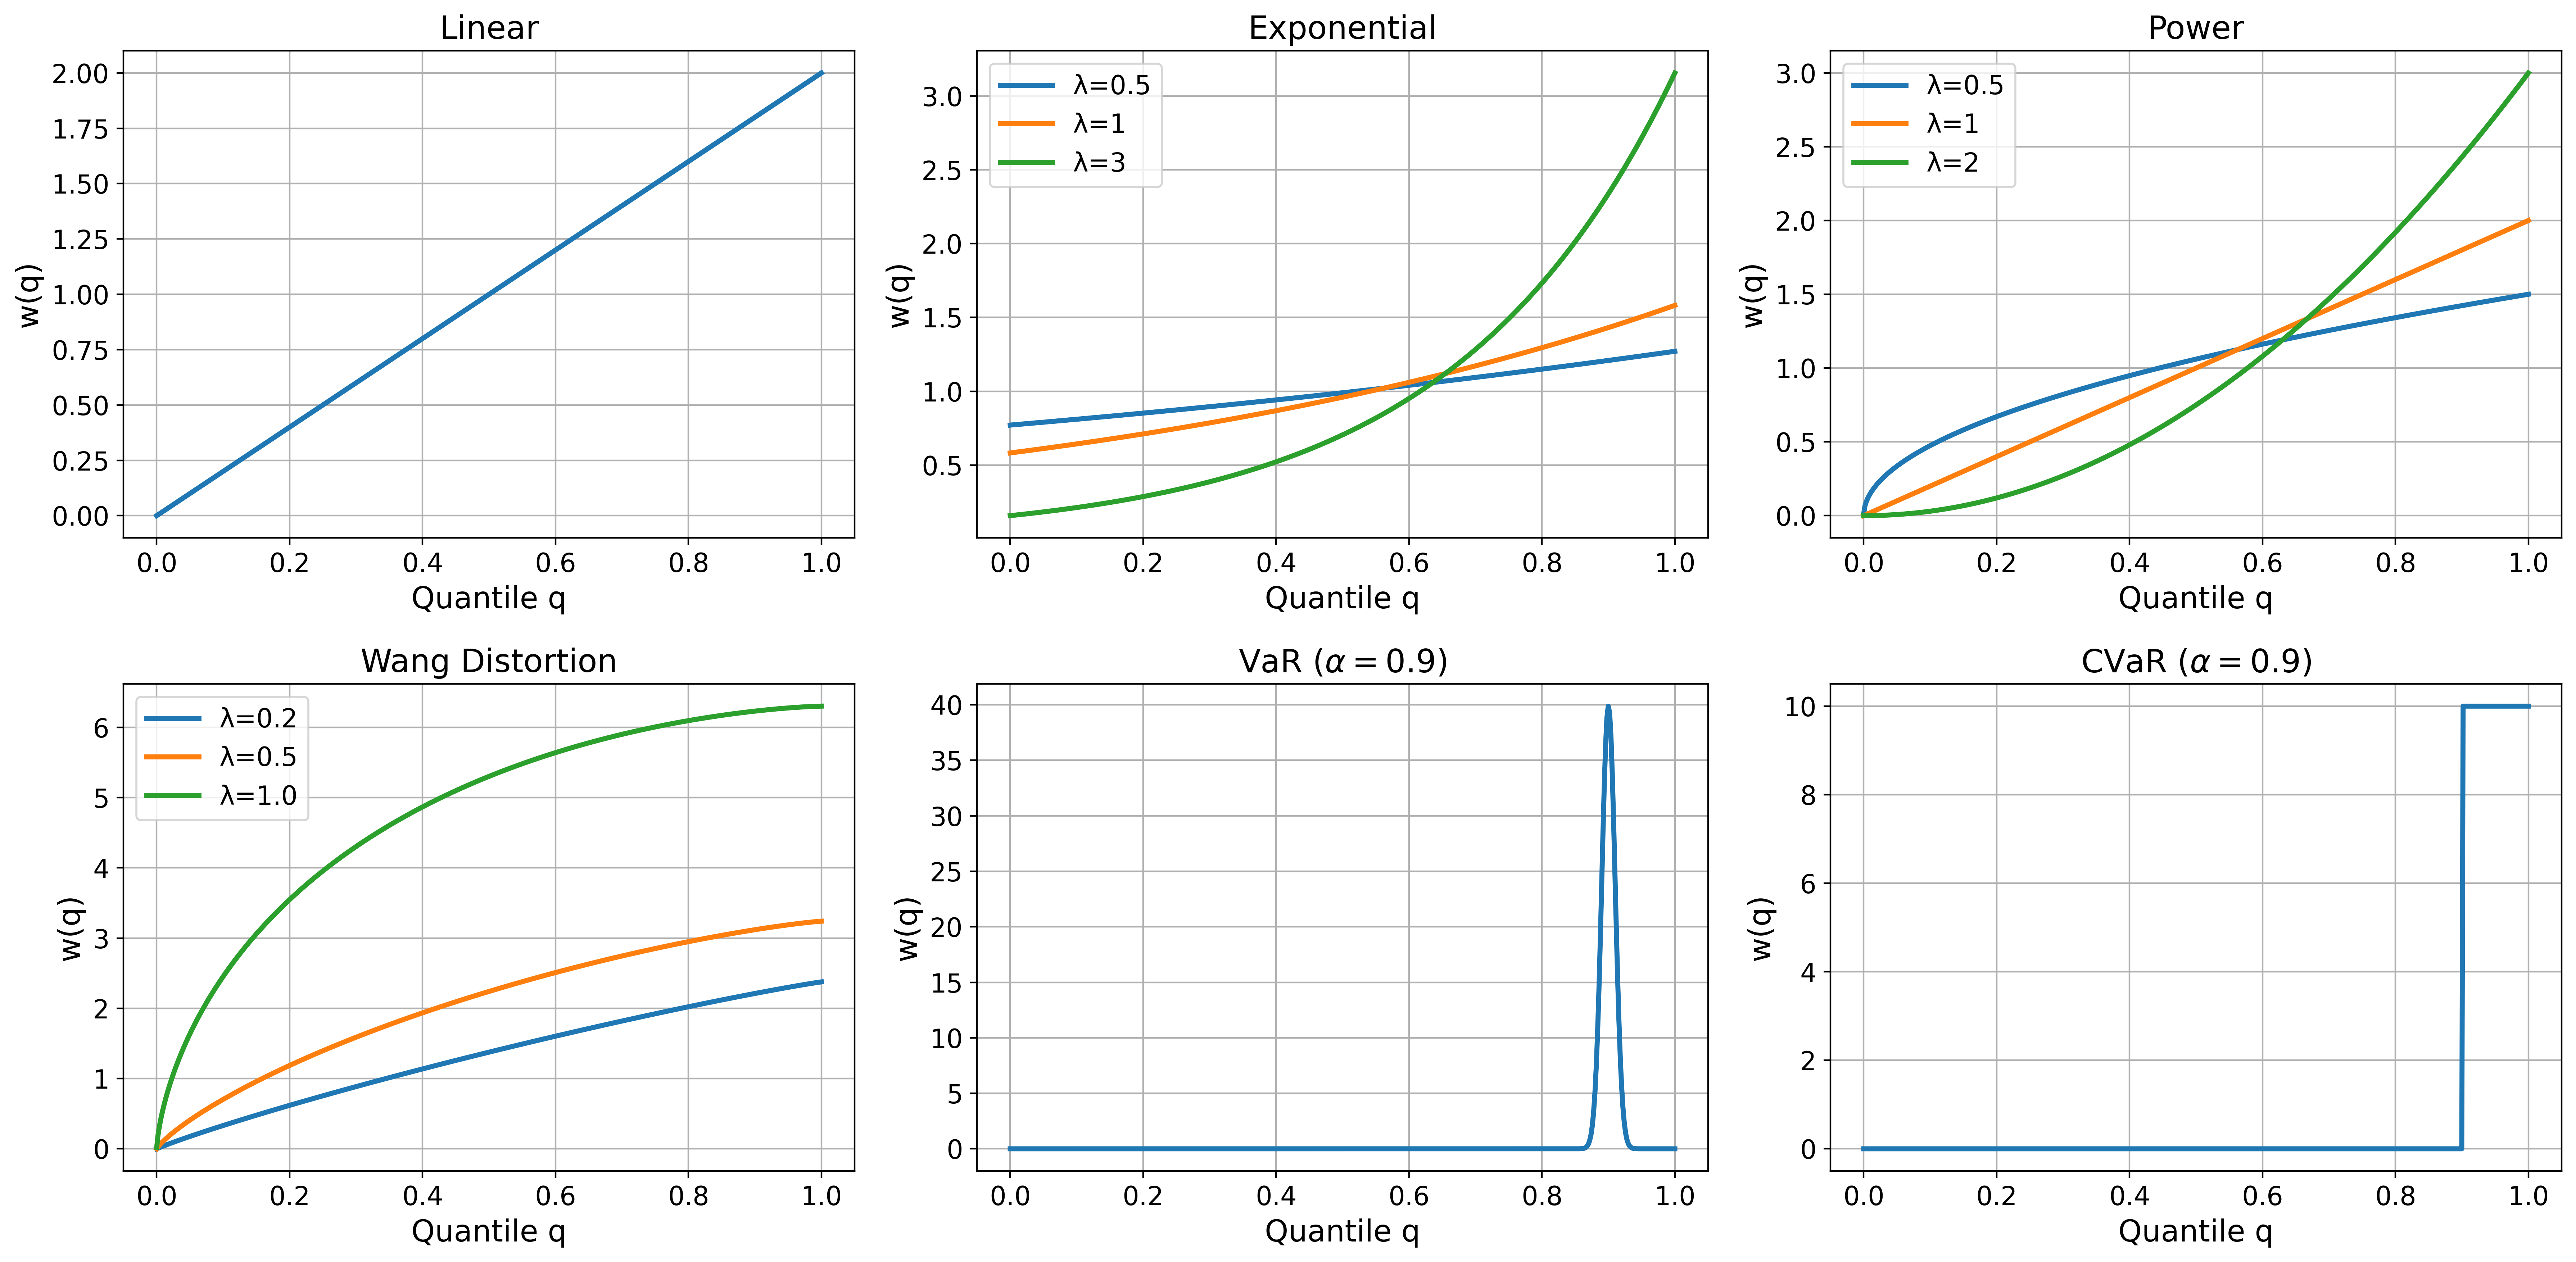
\includegraphics[width=0.9\textwidth]{figs/spectral_weights_comparison.png}
%     \caption{Illustration of spectral weighting functions corresponding to different spectral risk measures (SRMs). For parameterized families, the plots show how the spectral weights vary with the risk-aversion parameter $\lambda$.} \label{fig:srm-illustration}
% \end{figure}

% By selecting different quantile-weighting functions $w(q)$ in $\mathcal{L}_{\mathrm{FSD}}^w$, the FSD constraint can be tailored to enforce a variety of risk-sensitive behaviors. Uniform weights recover expected-cost minimization, extreme tail-focused weights recover Value-at-Risk or Conditional Value-at-Risk, and other schemes correspond to more general spectral risk measures. Thus, our framework provides a unified mechanism to impose different risk profiles simply by choosing $w(q)$, enabling principled, risk-aware alignment of policy behavior.


\section{Empirical Results}
\label{sec: results}
We investigate the following research questions: [Q1] \emph{How do models aligned using RAD compare to methods that enforce safety via expected cost constraints, in terms of helpfulness and harmfulness?} [Q2] \emph{How do RAD-aligned models perform against baselines wrt harmlessness of responses, on out-of-distribution data?}

We follow the standard RLHF pipeline for alignment. As our base model, we use Qwen2.5-3B \citep{qwen2025qwen25technicalreport}. We first fine-tune this model on the Alpaca dataset \citep{alpaca} \raj{citation?} to obtain the SFT initialization. For reward and cost modeling, we use the BeaverTails dataset~\citep{ji2023beavertailsimprovedsafetyalignment}, which provides pairwise preference annotations along two dimensions: helpfulness and harmfulness. The helpfulness preferences are used to train a reward model, while the harmfulness preferences are used to train a cost model. Both models are trained using the standard Bradley-Terry objective \citep{bradley1952rank} in \Cref{eq:bt_rm_loss}. Importantly, we adopt the same fine-tuning and reward/cost modeling procedure used in Safe RLHF~\citep{dai2023safe}, ensuring a controlled comparison.

In the RL stage, RAD employs a REINFORCE-based policy gradient method, using \Cref{eq:sard_pg}, with RLOO (Leave-One-Out) baseline and two sampled responses per prompt ($k = 2$). Additional implementation
details, including hyperparameters, are provided in supplementary material \ref{supp:implementation-details}. We set $\kappa=10$ for our RAD optimization objective in 
\Cref{eq:sard_primal_constr}. To provide a fair comparison with the baselines, we set the Safe-RLHF cost threshold $\tau=-10$ in \Cref{eq:safe-rlhf-obj}, following Corollary~\ref{cor:srm-fsd-relation}, since we observed $\mathbb{E}_{x \sim \mathcal{D}, y \sim 
\pi_{\textrm{ref}}(\cdot\vert x)}[c_{\psi}(x,y)] \approx 0$.

\subsection{Model Evaluations}

We compare models aligned using RAD and Safe RLHF using the same reward and cost models trained on BeaverTails preferences~\citep{ji2023beavertailsimprovedsafetyalignment}. Since RAD is a dominance based alignment framework rather than a single objective, we train multiple models corresponding to different spectral weighting schemes over the quantiles in the FSD objective. These weighting schemes are listed in Table~\ref{tab:spectral_weights}.

We evaluate the helpfulness and harmlessness of all model responses, using the prompts in the test set of BeaverTails. We adopt a pairwise evaluation protocol in which we designate one model as the \emph{blue} model and another as the \emph{red} model. Typically, the \emph{red} model represents a baseline (Safe RLHF or SFT) and the \emph{blue} model represents a RAD variant, though this assignment can vary across comparisons.

\paragraph{Harmlessness}

We use the trained cost model to judge the harmlessness of model generations for all considered approaches. From Table~\ref{tab:safe-response-prop}, RAD models achieve a higher proportion of safe responses compared to both baselines -- SFT and
Safe RLHF -- highlighting the benefits of enforcing distributional dominance constraints over expected cost alone.

\begin{table}[t]
  \centering
  {\footnotesize
    % \begin{tabular}{p{4cm} p{2.5cm} p{2.5cm} p{1.5cm} p{1.5cm}}
    \begin{tabular}{>{\centering\arraybackslash}p{4cm} >{\centering\arraybackslash}p{2.5cm} >{\centering\arraybackslash}p{2.5cm} >{\centering\arraybackslash}p{1.5cm} >{\centering\arraybackslash}p{1.5cm}}
      \toprule
      \makecell{Competition \\ (Red vs Blue)} & 
        \makecell{Reward of Blue \\ Higher} & 
        \makecell{Reward of Blue \\ Lower} & 
        \makecell{Overall \\ Blue} & 
        \makecell{Overall \\ Red} \\
      % Competition (Red vs Blue) & Reward of Blue Higher & Reward of Blue Lower & Overall Blue & Overall Red\\
      % & {}
      % & Higher
      % & Lower
      % & {}
      % & {}
      % \\
      \midrule
      safe-rlhf vs fsd-uniform             & $0.96\pm0.01$ & $0.83\pm0.14$ & $0.92\pm0.05$ & \underline{\textbf{$0.93\pm0.00$}} \\
      safe-rlhf vs fsd-var                 & $0.88\pm0.10$ & $0.88\pm0.10$ & $0.88\pm0.10$ & \underline{\textbf{$0.93\pm0.00$}} \\
      safe-rlhf vs fsd-cvar                & $0.96\pm0.00$ & $0.98\pm0.00$ & \underline{\textbf{$0.97\pm0.00$}} & $0.93\pm0.00$ \\
      safe-rlhf vs fsd-spectral-linear     & $0.97\pm0.00$ & $0.93\pm0.04$ & \underline{\textbf{$0.94\pm0.03$}} & $0.93\pm0.00$ \\
      safe-rlhf vs fsd-spectral-wang       & $0.97\pm0.01$ & $0.95\pm0.00$ & \underline{\textbf{$0.96\pm0.00$}} & $0.93\pm0.00$ \\
      safe-rlhf vs fsd-spectral-power      & $0.97\pm0.01$ & $0.94\pm0.02$ & \underline{\textbf{$0.96\pm0.01$}} & $0.93\pm0.00$ \\
      safe-rlhf vs fsd-spectral-exponential& $0.98\pm0.01$ & $0.94\pm0.03$ & \underline{\textbf{$0.96\pm0.01$}} & $0.93\pm0.00$ \\
      \midrule
      sft vs fsd-uniform                   & $0.95\pm0.03$ & $0.65\pm0.16$ & \underline{\textbf{$0.92\pm0.05$}} & $0.55\pm0.00$ \\
      sft vs fsd-var                       & $0.93\pm0.06$ & $0.82\pm0.10$ & \underline{\textbf{$0.88\pm0.10$}} & $0.55\pm0.00$ \\
      sft vs fsd-cvar                      & $0.98\pm0.00$ & $0.92\pm0.01$ & \underline{\textbf{$0.97\pm0.01$}} & $0.55\pm0.00$ \\
      sft vs fsd-spectral-linear           & $0.97\pm0.01$ & $0.74\pm0.15$ & \underline{\textbf{$0.94\pm0.03$}} & $0.55\pm0.00$ \\
      sft vs fsd-spectral-wang             & $0.97\pm0.00$ & $0.75\pm0.03$ & \underline{\textbf{$0.96\pm0.00$}} & $0.55\pm0.00$ \\
      sft vs fsd-spectral-power            & $0.97\pm0.01$ & $0.76\pm0.08$ & \underline{\textbf{$0.95\pm0.01$}} & $0.55\pm0.00$ \\
      sft vs fsd-spectral-exponential      & $0.98\pm0.01$ & $0.66\pm0.17$ & \underline{\textbf{$0.96\pm0.01$}} & $0.55\pm0.00$ \\
      \midrule
      sft vs safe-rlhf                     & $0.96\pm0.00$ & $0.61\pm0.03$ & \underline{\textbf{$0.93\pm0.00$}} & $0.55\pm0.00$ \\
      \bottomrule
    \end{tabular}
  }
  \caption{
    Comparison of the proportion of safe responses produced by the blue model, as judged by the cost model, across competing model pairs. We further decompose this proportion into two subsets based on whether the blue model's response achieved higher reward than the red model's response (first two columns). The ``Overall Blue'' column reports the overall proportion of safe responses for the blue model, while the ``Overall Red'' column reports the same for the red model. We observe that RAD-aligned models consistently produce a higher proportion of safe responses than the baselines, as evidenced by the comparison of the final two columns. Values are reported as mean $\pm$ standard deviation across 3 random seeds.
    % \vspace{-0.3in}
  }
  \label{tab:safe-response-prop}
\end{table}


% \begin{table}[t]
%   \centering
%   {\footnotesize
%     \begin{tabular}{p{4.5cm} p{2.5cm} p{2.5cm} p{1.5cm} p{1.5cm}}
%       \toprule
%       Competetion (Red vs Blue) & Reward of Blue Higher & Reward of Blue Lower & Overall Blue & Overall Red\\
%       \midrule
%       safe-rlhf vs fsd-uniform & 0.96 & 0.94 & \underline{\textbf{0.94}} & 0.93  \\
%       safe-rlhf vs fsd-var &  0.95 & 0.96 & \underline{\textbf{0.96}} & 0.93  \\
%       safe-rlhf vs fsd-cvar & 0.96 & 0.98 & \underline{\textbf{0.97}} & 0.93   \\
%       safe-rlhf vs fsd-spectral-linear & 0.97 & 0.87 & 0.91 & \underline{\textbf{0.93}}   \\
%       safe-rlhf vs fsd-spectral-power & 0.96 & 0.93 & \underline{\textbf{0.94}} & 0.93   \\
%       safe-rlhf vs fsd-spectral-wang & 0.98 & 0.94 & \underline{\textbf{0.96}} & 0.93  \\
%       safe-rlhf vs fsd-spectral-exponential & 0.98 & 0.95 & \underline{\textbf{0.96}} & 0.93   \\
%       sft vs fsd-uniform & 0.97 & 0.79 & \underline{\textbf{0.94}} & 0.56   \\
%       sft vs fsd-var & 0.97 & 0.88 & \underline{\textbf{0.96}} & 0.55   \\
%       sft vs fsd-cvar & 0.98 & 0.92 & \underline{\textbf{0.97}} & 0.55  \\
%       sft vs fsd-spectral-linear & 0.96 & 0.54 & \underline{\textbf{0.91}} & 0.55   \\
%       sft vs fsd-spectral-power & 0.96 & 0.71 & \underline{\textbf{0.94}} & 0.55  \\
%       sft vs fsd-spectral-wang & 0.98 & 0.71  & \underline{\textbf{0.96}} & 0.56 \\
%       sft vs fsd-spectral-exponential & 0.98 & 0.77 & \underline{\textbf{0.96}} & 0.55   \\
%       sft vs safe-rlhf & 0.96 & 0.64 & \underline{\textbf{0.93}} & 0.55 \\
%       \bottomrule
%     \end{tabular}
%   }
%   \caption{
%     Comparison of the proportion of safe responses produced by the blue model, as judged by the cost model, across competing model pairs. We further decompose this proportion into two subsets based on whether the blue model's response achieved higher reward than the red model's response (first two columns). The ``Overall Blue'' column reports the overall proportion of safe responses for the blue model, while the ``Overall Red'' column reports the same for the red model. We observe that RAD-aligned models consistently produce a higher proportion of safe responses than the baselines, as evidenced by the comparison of the final two columns. \yc{Might need to comment on spectral linear? Worst case remove}
%     % \vspace{-0.3in}
%   }
%   \label{tab:safe-response-prop}
% \end{table}

Let $C_{\pi_{\textrm{blue}}}$ and $C_{\pi_{\textrm{red}}}$ denote the random variables corresponding to the cost distributions induced by the blue and red models, respectively. We define the dominance difference as
\[
  D_{\textrm{FSD}}^{w}(C_{\pi_{\textrm{blue}}}, C_{\pi_{\textrm{red}}}) :=
  \mathcal{L}_{\textrm{FSD}}^{w}(C_{\pi_{\textrm{blue}}}, C_{\pi_{\textrm{red}}})
  - \mathcal{L}_{\textrm{FSD}}^{w}(C_{\pi_{\textrm{red}}}, C_{\pi_{\textrm{blue}}}).
\]

Intuitively, for the blue model to have a safer cost distribution than the red model, we would want
$\mathcal{L}_{\textrm{FSD}}^{w}(C_{\pi_{\textrm{blue}}}, C_{\pi_{\textrm{red}}})$ to be high and
$\mathcal{L}_{\textrm{FSD}}^{w}(C_{\pi_{\textrm{red}}}, C_{\pi_{\textrm{blue}}})$ to be low.
This implies a high positive $D_{\textrm{FSD}}^{w}(C_{\pi_{\textrm{blue}}}, C_{\pi_{\textrm{red}}})$.

We compare the competing models using $D_{\textrm{FSD}}^{w}(C_{\pi_{\textrm{blue}}}, C_{\pi_{\textrm{red}}})$, reporting both the weighted and unweighted dominance difference. The weighted dominance difference corresponds to the difference in spectral risk measures under the chosen weighting: a positive value indicates a reduction in the weighted spectral risk measure for the blue model compared to the red model. The unweighted dominance difference corresponds to the difference in average cost: a positive value indicates a lower average cost for the blue model relative to the red model. Table~\ref{tab:cost-dominance} presents the dominance results.
We use an unnormalized weighting in the Dominance Difference; this does not affect the results, as all values are scaled by a constant factor for a fixed weighting.
% Importantly, RAD's improvements are consistent across multiple weighting functions, suggesting that its effectiveness is not tied to any particular risk metric. Practitioners can therefore select the weighting function that best reflects their deployment context and risk tolerance — for instance, preferring CVaR-style weightings in high-stakes settings or uniform weighting when average cost reduction is the primary objective.

% We compare the competing models using $D_{\textrm{FSD}}^{w}(C_{\pi_{\textrm{blue}}}, C_{\pi_{\textrm{red}}})$, reporting both the weighted and unweighted dominance difference. The weighted dominance difference corresponds to the difference in spectral risk measures under the chosen weighting: a positive value indicates a reduction in the weighted spectral risk measure for the blue model compared to the red model. The unweighted dominance difference corresponds to the difference in average cost: a positive value indicates a lower average cost for the blue model relative to the red model. Table~\ref{tab:cost-dominance} presents the dominance results.
% We use an unnormalized weighting; this does not affect the results, as all values are scaled by a constant factor for a fixed weighting.

% From Table \ref{tab:cost-dominance}, we observe that most models aligned with RAD, using different quantile weighting functions, have a positive weighted dominance metric compared to baselines. This implies a reduction in the spectral risk measure of the RAD aligned models compared to baselines. The higher proportion of safe reponses and positive weighted dominance difference metric point out the benifits of using distributional dominance constraints, compared to methods that use a central statistic of the distribution (such as expectation) to enforce safety. Importantly, RAD's improvements are consistent across multiple weighting functions, suggesting that its effectiveness is not tied to any particular risk metric. Practitioners can therefore select the weighting function that best reflects their deployment context and risk tolerance — for instance, preferring CVaR-style weightings in high-stakes settings or uniform weighting when average cost reduction is the primary objective.

From Table~\ref{tab:cost-dominance}, we observe that most RAD models, across different quantile weighting functions, achieve a positive weighted dominance metric relative to the baselines, implying a  reduction in the corresponding spectral risk measure. Together with the higher proportion of safe responses, these results demonstrate the benefits of enforcing distributional dominance constraints over
methods that constrain only a central statistic of the cost distribution, such as the expected cost. Importantly, RAD's improvements are consistent across multiple weighting functions, suggesting that its effectiveness is not tied to any particular risk
metric. Practitioners can therefore select the weighting function that best reflects their deployment context and risk tolerance --
for instance, preferring CVaR-style weightings in high-stakes settings or uniform weighting when average cost reduction is the primary objective.

\begin{table}[t]
  \centering
  {\footnotesize
    \begin{tabular}{lcc}
      \toprule
      Competetion (Red vs Blue) & $D_{\textrm{FSD}}(C_{\pi_{\textrm{blue}}}, C_{\pi_{\textrm{red}}})$ & $D_{\textrm{FSD}}^{w}(C_{\pi_{\textrm{blue}}}, C_{\pi_{\textrm{red}}})$ \\
      \midrule
      safe-rlhf vs fsd-uniform & $+7.92 \pm 11.23$ & \underline{\textbf{$+7.92 \pm 11.23$}} \\
      safe-rlhf vs fsd-var & $-66.06 \pm 46.66$ & $-2.95 \pm 10.93$ \\
      safe-rlhf vs fsd-cvar & $-12.54 \pm 2.80$ & \underline{\textbf{$+56.61 \pm 10.39$}} \\
      safe-rlhf vs fsd-spectral-linear & $-7.33 \pm 7.63$ & $-0.49 \pm 11.59$ \\
      safe-rlhf vs fsd-spectral-wang & $+5.74 \pm 5.00$ & \underline{\textbf{$+27.91 \pm 14.99$}} \\
      safe-rlhf vs fsd-spectral-power & $-3.50 \pm 6.34$ & \underline{\textbf{$+9.45 \pm 8.67$}} \\
      safe-rlhf vs fsd-spectral-exponential & $+8.18 \pm 11.04$ & \underline{\textbf{$+22.16 \pm 10.04$}} \\
      \midrule
      sft vs fsd-uniform & $+147.12 \pm 12.43$ & \underline{\textbf{$+147.12 \pm 12.43$}} \\
      sft vs fsd-var & $+73.06 \pm 46.52$ & \underline{\textbf{$+17.59 \pm 10.83$}} \\
      sft vs fsd-cvar & $+126.84 \pm 1.68$ & \underline{\textbf{$+139.83 \pm 7.52$}} \\
      sft vs fsd-spectral-linear & $+131.24 \pm 11.22$ & \underline{\textbf{$+135.64 \pm 15.54$}} \\
      sft vs fsd-spectral-wang & $+144.63 \pm 1.56$ & \underline{\textbf{$+432.69 \pm 4.63$}} \\
      sft vs fsd-spectral-power & $+135.91 \pm 5.54$ & \underline{\textbf{$+134.40 \pm 3.95$}} \\
      sft vs fsd-spectral-exponential & $+147.88 \pm 9.84$ & \underline{\textbf{$+145.47 \pm 9.59$}} \\
      \midrule
      sft vs safe-rlhf & $+138.51 \pm 2.45$ & - \\
      \bottomrule
    \end{tabular}
  }
  \caption{
    Unweighted and weighted dominance differences for all pairs of competing models.
    A positive weighted dominance difference for the blue model indicates a reduction in the corresponding spectral risk measure relative to the red model. The weighted dominance difference uses the weighting corresponding to the blue model. Some weighting schemes (e.g., CVaR and VaR) exhibit negative unweighted dominance differences but positive weighted dominance differences.
    This occurs because CVaR only weights the higher quantiles while setting others to zero, and VaR is a Dirac mass at a particular quantile (Gaussian-smoothed for implementation purposes), disregarding other quantiles. Values are reported as mean $\pm$ standard deviation across 3 random seeds.
  }
  % \caption{Unweighted and Weighted dominance difference for all all pairs of competing models. We observe that blue models have a positive weighted domianance difference metric, implying a reducing in the correpondiong spectral risk measure for the blue model against the red model. We also point out that some weighting schemes (such as CVaR, VaR) have negative unweighted dominace metric, but a positive weighted dominance metric. This is because CVaR only weighhs the higher qiantiles while keeping others zero, and VaR is just a dirac mass at a particular quantile (gaussian smoothened for implementation)}
  \label{tab:cost-dominance}
\end{table}

\paragraph{Helpfulness}

We use the trained reward model, to judge the helpfulness of model generations for all the approaches we consider. We compute the reward win-rates, pitting two models against each other, with their response helpfulness judged by the reward model, which assigns a higher score to more helpful responses. The results are shown in Figure \ref{fig:reward-winrates-test}. In each cell, in addition to win rate, we also provide the count of the number of responses compared. Each row corresponds to a pairwise competition (red vs. blue). We report the reward win rate of the blue model, defined as the percentage of prompts for which the blue model's response achieves higher reward than the red model's response. The x-axis partitions results by safety outcome combinations of the two models: (safe, safe), (safe, unsafe), (unsafe, safe), and (unsafe, unsafe), where the first entry corresponds to the red model and the second to the blue model. For example, (safe, unsafe) denotes the subset of prompts where the red model produces a safe response and the blue model produces an unsafe response. The final column reports the overall win rate across all prompts. 

From Figure~\ref{fig:reward-winrates-test}, RAD-aligned models achieve higher rewards than the SFT baseline, as evidenced by consistently high reward win rates. Against Safe-RLHF, FSD-VaR, FSD-CVaR, and FSD-Spectral-Linear obtain lower reward win rates, suggesting these weighting schemes are more risk-averse at the expense of helpfulness -- a tradeoff that may be desirable in risk-sensitive deployment contexts such as medical or legal applications. The remaining variants achieve comparable reward win rates against Safe-RLHF, indicating helpfulness parity.


% In particular, Spectral-Wang achieves a 53\% overall reward win rate against Safe RLHF, marginally above the 50\% threshold. Spectral-Exponential and Spectral-Power achieve win rates of 49\% and 48\%, respectively, when compared against Safe RLHF, placing them close to parity. The remaining FSD variants obtain lower reward win rates against
% Safe RLHF, suggesting that these weighting schemes place greater emphasis on harmlessness at the expense of helpfulness. This tradeoff may be desirable in risk-sensitive deployment contexts -- such as medical or legal applications -- where the cost of harmful
% outputs outweighs the cost of reduced helpfulness.

% \paragraph{Summary}
% From the results on the harmlessness and helpfulness of model responses, we observe that SARD-aligned methods produce a higher proportion of safe responses compared to the baselines, and exhibit a higher positive weighted dominance difference, implying a reduction in spectral risk relative to the baselines.
% We additionally observe that certain spectral weighting schemes (Spectral-Wang, Spectral-Power, Spectral-Exponential) achieve either parity or marginally higher helpfulness compared to the baselines.
% Overall, RAD-aligned methods perform well on both helpfulness and harmlessness, demonstrating that they can match or marginally improve helpfulness of model responses, while simultaneously reducing risk.

\paragraph{Summary}
From the results on the harmlessness and helpfulness of model responses, we observe that RAD-aligned methods produce a higher proportion of safe
responses compared to the baselines, and exhibit a higher positive weighted dominance difference, implying a reduction in spectral risk relative to the baselines. Furthermore, for spectral weighting schemes -- specifically Spectral-Wang, Spectral-Power, Spectral-Exponential, and uniform
-- these gains in safety are made while maintaining parity in helpfulness with Safe RLHF.

\begin{figure}  % 'r' for right-aligned figure
  \centering
  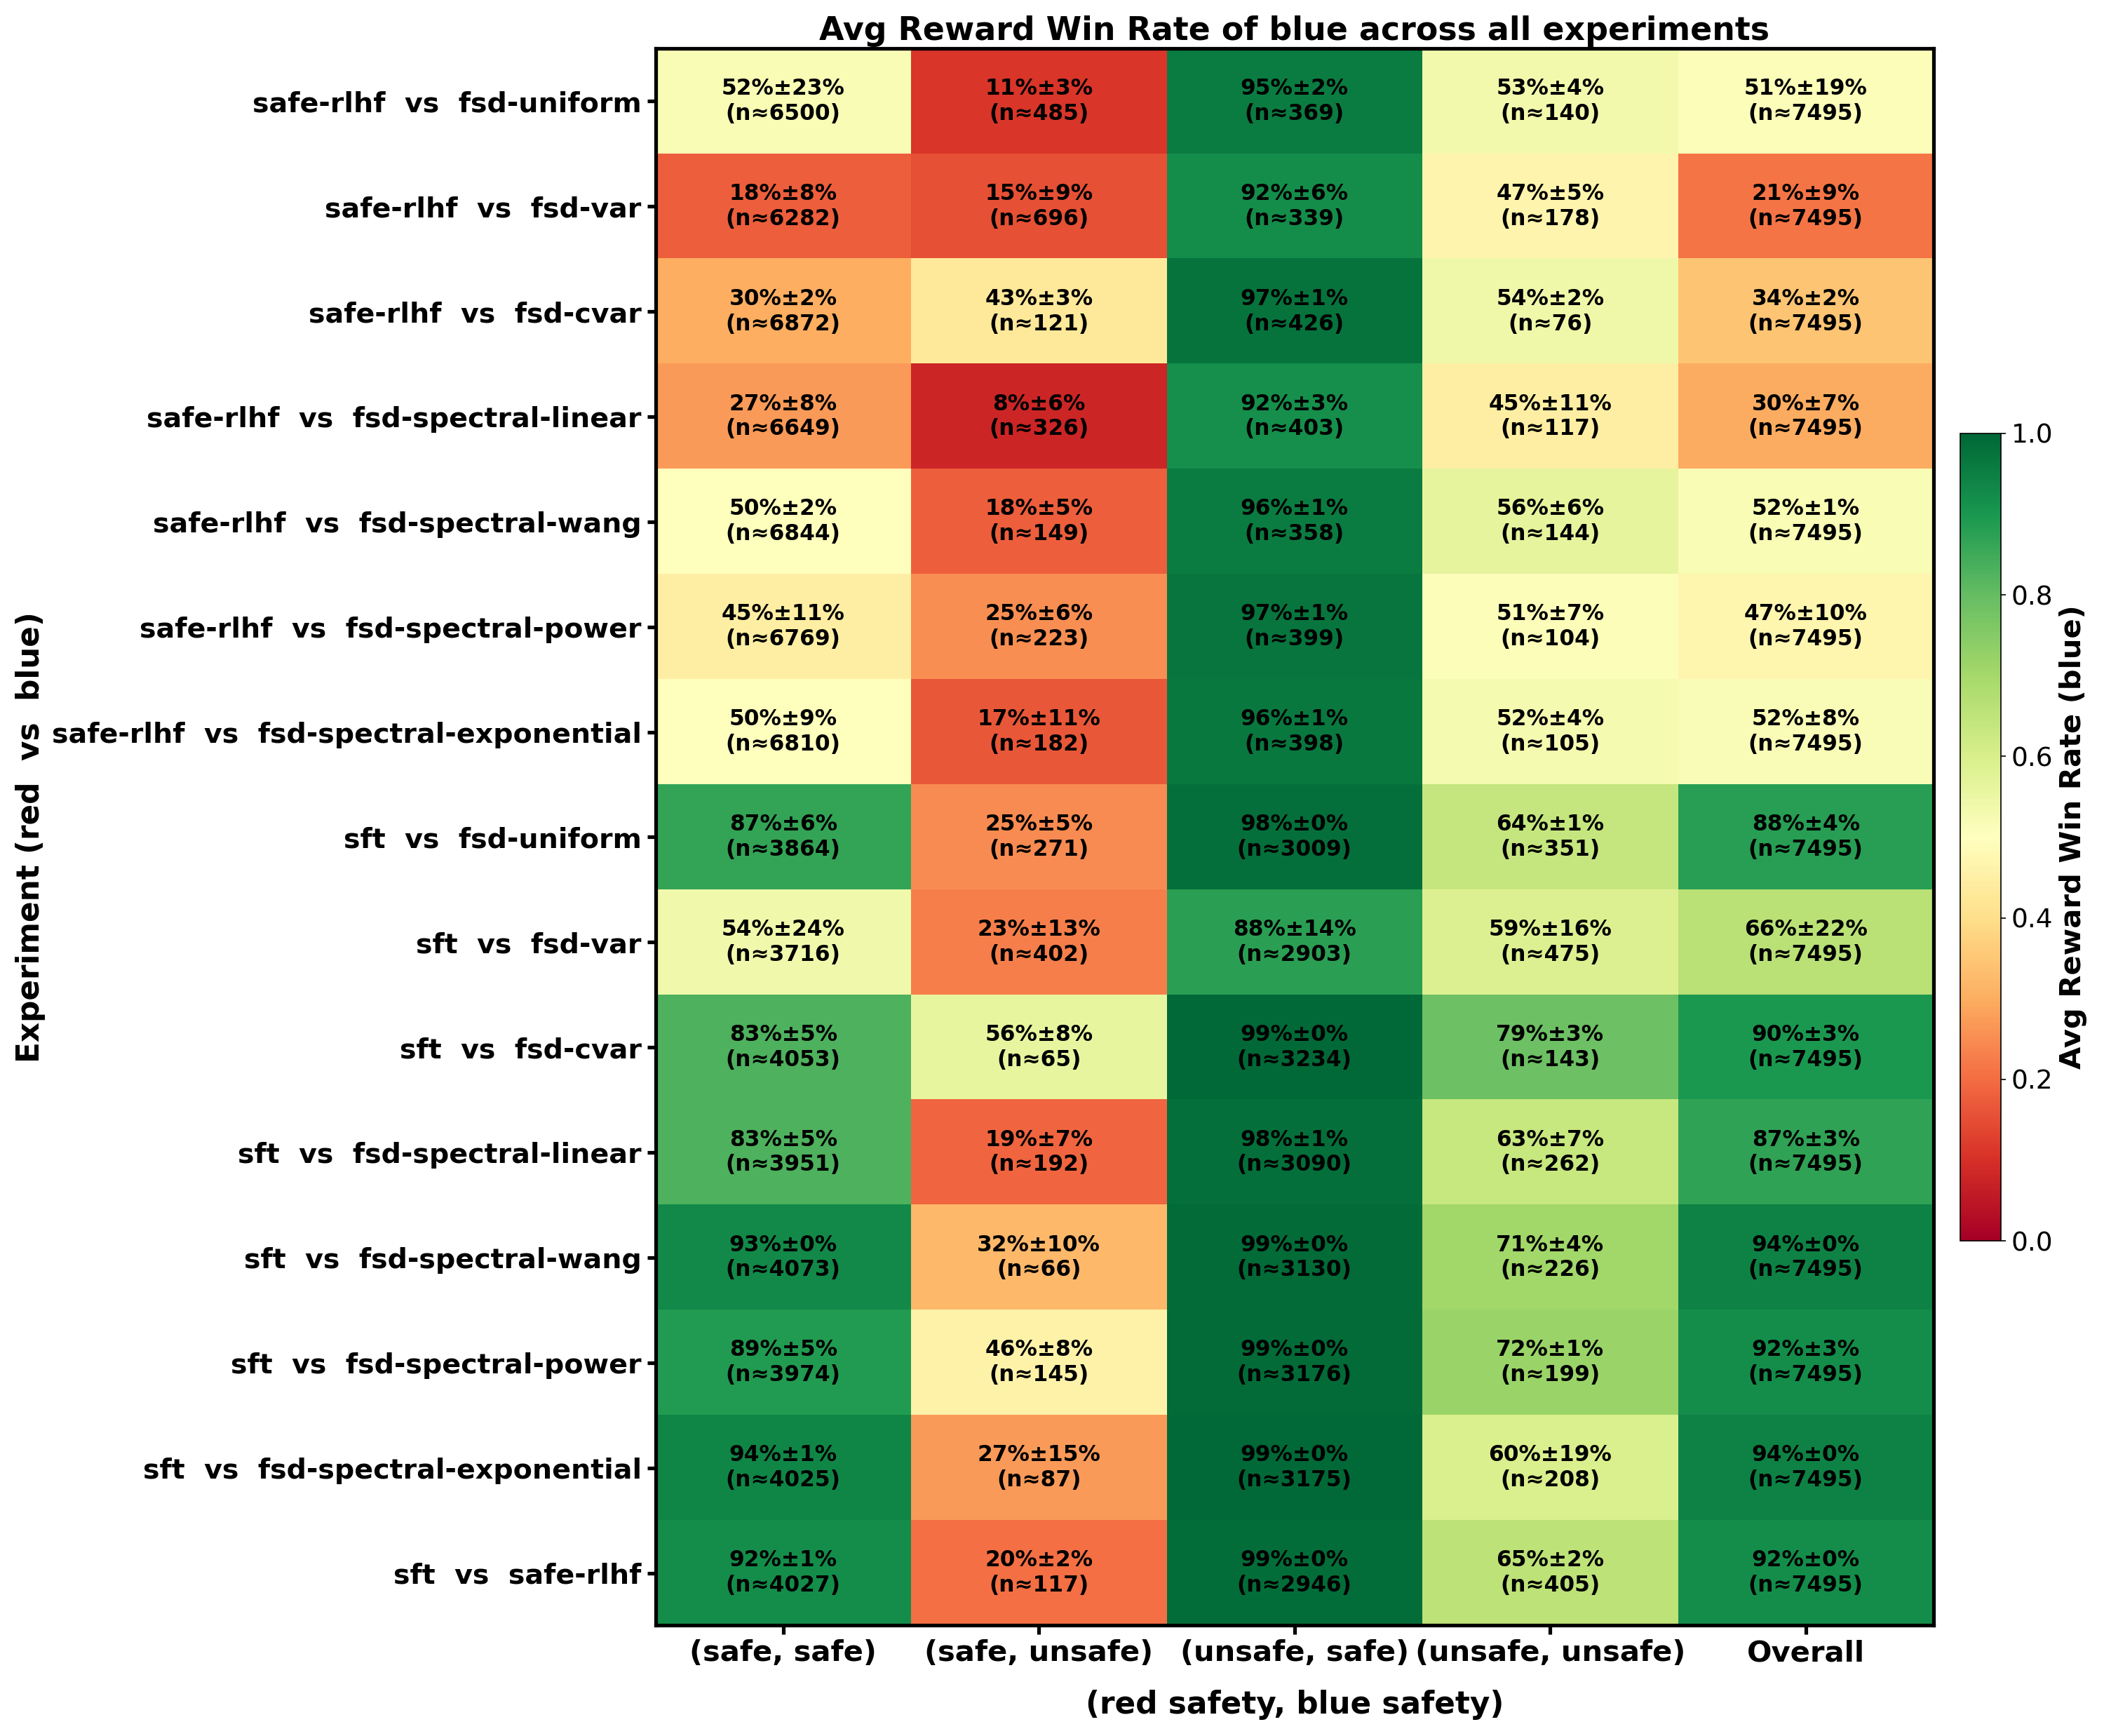
\includegraphics[width=0.9\textwidth]{./figs/summary_heatmap_averaged.png}
  \caption{
     Average reward win rates between competing models, across 3 seeds.
  }
  \label{fig:reward-winrates-test}
\end{figure}

\subsection{Out-of-Distribution Harmlessness: HarmBench Evaluation}

To assess generalization beyond the training distribution, we evaluate
all models on HarmBench \citep{mazeika2024harmbenchstandardizedevaluationframework}, an out-of-distribution
red-teaming benchmark comprising adversarially constructed harmful prompts
across diverse risk categories. Critically, neither the reward model, cost
model, nor any model checkpoint was trained or selected using HarmBench
data, making this a clean held-out evaluation.

We use GPT-4o-mini \citep{openai2024gpt4omini} as an independent pairwise harmlessness judge,
following standard LLM-as-a-judge \citep{zheng2023judgingllmasajudgemtbenchchatbot} evaluation protocol \cite{}. For each
prompt, the judge compares responses from two models and determines which
is less harmful. We provide the GPT evaluation results in \Cref{tab:harmbench-gpt-eval}

All RAD variants substantially outperform the SFT baseline, confirming that our constrained RL training, with the SFT policy as the reference, improves harmlessness and generalizes to unseen prompts.  Against Safe-RLHF, spectral variants -- Spectral-Power, Spectral-Exponential, Spectral-Linear, CVaR, and VaR -- achieve favorable win-loss ratios, suggesting that upweighting the tail of the cost distribution confers greater robustness to distributional shift. 

% \paragraph{Comparison against SFT.} All FSD variants substantially
% outperform the SFT baseline, with win rates ranging from 65.0\% to
% 82.4\% and loss rates below 31\%. This confirms that constrained RL
% training meaningfully improves harmlessness over supervised fine-tuning
% alone, and that this improvement generalizes to prompts unseen during
% training.

% \paragraph{Comparison against Safe RLHF.} Results are more nuanced
% when comparing against Safe RLHF. Some FSD variants — namely
% fsd-spectral-wang, fsd-spectral-exponential, fsd-spectral-power, fsd-spectral-linear, and fsd-cvar —
% achieve favorable win-loss ratios, indicating improved harmlessness
% generalization on OOD prompts. This suggests that spectral risk measures, which weight the
% tail of the cost distribution more heavily, confer greater robustness
% to distributional shift — consistent with our theoretical motivation for
% FSD-based constraints. Var should be in this list, but we obsderved that VaR suffers from unstable optimization, due to the dirac mass weighting

\begin{table}[t]
  \centering
  {\footnotesize
    \begin{tabular}{lcc}
      \toprule
      Model Name & SFT & Safe RLHF \\
      \midrule
      fsd-uniform & \underline{\textbf{67.1\%}}{\scriptsize$\pm$2.1} / 7.8\%{\scriptsize$\pm$4.2} / 25.1\%{\scriptsize$\pm$6.3} & 38.0\%{\scriptsize$\pm$6.9} / 22.2\%{\scriptsize$\pm$15.0} / \underline{\textbf{39.8\%}}{\scriptsize$\pm$8.4} \\
      fsd-var & \underline{\textbf{76.6\%}}{\scriptsize$\pm$3.7} / 10.6\%{\scriptsize$\pm$2.7} / 12.7\%{\scriptsize$\pm$2.3} & \underline{\textbf{39.6\%}}{\scriptsize$\pm$10.6} / 28.6\%{\scriptsize$\pm$16.8} / 31.8\%{\scriptsize$\pm$9.7} \\
      fsd-cvar & \underline{\textbf{72.9\%}}{\scriptsize$\pm$2.4} / 15.7\%{\scriptsize$\pm$1.3} / 11.4\%{\scriptsize$\pm$2.4} & \underline{\textbf{28.6\%}}{\scriptsize$\pm$7.8} / 46.5\%{\scriptsize$\pm$2.1} / 24.9\%{\scriptsize$\pm$6.6} \\
      fsd-spectral-linear & \underline{\textbf{75.3\%}}{\scriptsize$\pm$6.3} / 12.3\%{\scriptsize$\pm$2.0} / 12.4\%{\scriptsize$\pm$5.1} & \underline{\textbf{34.2\%}}{\scriptsize$\pm$2.8} / 37.0\%{\scriptsize$\pm$12.8} / 28.9\%{\scriptsize$\pm$13.4} \\
      fsd-spectral-wang & \underline{\textbf{67.3\%}}{\scriptsize$\pm$7.9} / 13.4\%{\scriptsize$\pm$0.6} / 19.3\%{\scriptsize$\pm$7.9} & 24.7\%{\scriptsize$\pm$1.7} / 49.7\%{\scriptsize$\pm$7.4} / \underline{\textbf{25.5\%}}{\scriptsize$\pm$8.1} \\
      fsd-spectral-exponential & \underline{\textbf{74.7\%}}{\scriptsize$\pm$1.6} / 12.6\%{\scriptsize$\pm$1.2} / 12.7\%{\scriptsize$\pm$1.6} & \underline{\textbf{28.0\%}}{\scriptsize$\pm$6.1} / 52.2\%{\scriptsize$\pm$7.0} / 19.9\%{\scriptsize$\pm$2.2} \\
      fsd-spectral-power & \underline{\textbf{71.0\%}}{\scriptsize$\pm$2.7} / 14.8\%{\scriptsize$\pm$2.1} / 14.1\%{\scriptsize$\pm$4.1} & \underline{\textbf{30.4\%}}{\scriptsize$\pm$2.0} / 48.9\%{\scriptsize$\pm$1.1} / 20.7\%{\scriptsize$\pm$2.7} \\
      \midrule
      Safe RLHF & \underline{\textbf{68.1\%}}{\scriptsize$\pm$2.6} / 20.4\%{\scriptsize$\pm$1.1} / 11.5\%{\scriptsize$\pm$2.5} & - \\
      \bottomrule
    \end{tabular}
  }
  \caption{
    Pairwise harmlessness evaluation on HarmBench using GPT-4o-mini as an independent judge. Each cell reports Win / Tie / Lose rates of the row model against the column model (mean $\pm$ std over 3 seeds). The dominant outcome -- win rate if the row model wins, loss rate if it loses -- is bold underlined. All FSD variants substantially outperform the SFT baseline. Against Safe RLHF, variants that upweight the tail (Eg: Exponential, Power, Linear, CVaR, and Var) achieve favorable win-loss ratios, demonstrating improved harmlessness generalization to out-of-distribution prompts.
  }
  \label{tab:harmbench-gpt-eval}
\end{table}


% \begin{table}[t]
%   \centering
%   {\footnotesize
%     \begin{tabular}{lcc}
%       \toprule
%       Model Name & SFT & Safe RLHF \\
%       \midrule
%       fsd-uniform & \underline{\textbf{67.1\%}}{\scriptsize$\pm$2.1} / 7.8{\scriptsize$\pm$4.2}\% / 25.1{\scriptsize$\pm$6.3}\% & 38.0{\scriptsize$\pm$6.9}\% / 22.2{\scriptsize$\pm$15.0}\% / \underline{\textbf{39.8\%}}{\scriptsize$\pm$8.4} \\
%       fsd-var & \underline{\textbf{76.6\%}}{\scriptsize$\pm$3.7} / 10.6{\scriptsize$\pm$2.7}\% / 12.7{\scriptsize$\pm$2.3}\% & \underline{\textbf{39.6\%}}{\scriptsize$\pm$10.6} / 28.6{\scriptsize$\pm$16.8}\% / 31.8{\scriptsize$\pm$9.7}\% \\
%       fsd-cvar & \underline{\textbf{72.9\%}}{\scriptsize$\pm$2.4} / 15.7{\scriptsize$\pm$1.3}\% / 11.4{\scriptsize$\pm$2.4}\% & \underline{\textbf{28.6\%}}{\scriptsize$\pm$7.8} / 46.5{\scriptsize$\pm$2.1}\% / 24.9{\scriptsize$\pm$6.6}\% \\
%       fsd-spectral-linear & \underline{\textbf{75.3\%}}{\scriptsize$\pm$6.3} / 12.3{\scriptsize$\pm$2.0}\% / 12.4{\scriptsize$\pm$5.1}\% & \underline{\textbf{34.2\%}}{\scriptsize$\pm$2.8} / 37.0{\scriptsize$\pm$12.8}\% / 28.9{\scriptsize$\pm$13.4}\% \\
%       fsd-spectral-wang & \underline{\textbf{67.3\%}}{\scriptsize$\pm$7.9} / 13.4{\scriptsize$\pm$0.6}\% / 19.3{\scriptsize$\pm$7.9}\% & 24.7{\scriptsize$\pm$1.7}\% / 49.7{\scriptsize$\pm$7.4}\% / \underline{\textbf{25.5\%}}{\scriptsize$\pm$8.1} \\
%       fsd-spectral-exponential & \underline{\textbf{74.7\%}}{\scriptsize$\pm$1.6} / 12.6{\scriptsize$\pm$1.2}\% / 12.7{\scriptsize$\pm$1.6}\% & \underline{\textbf{28.0\%}}{\scriptsize$\pm$6.1} / 52.2{\scriptsize$\pm$7.0}\% / 19.9{\scriptsize$\pm$2.2}\% \\
%       fsd-spectral-power & \underline{\textbf{71.0\%}}{\scriptsize$\pm$2.7} / 14.8{\scriptsize$\pm$2.1}\% / 14.1{\scriptsize$\pm$4.1}\% & \underline{\textbf{30.4\%}}{\scriptsize$\pm$2.0} / 48.9{\scriptsize$\pm$1.1}\% / 20.7{\scriptsize$\pm$2.7}\% \\
%       Safe RLHF & \underline{\textbf{68.1\%}}{\scriptsize$\pm$2.6} / 20.4{\scriptsize$\pm$1.1}\% / 11.5{\scriptsize$\pm$2.5}\% & - \\
%       \bottomrule
%     \end{tabular}
%   }
%   \caption{
%     Pairwise harmlessness evaluation on HarmBench using GPT-4o-mini as an independent judge. Each cell reports Win / Tie / Lose rates of the row model against the column model (mean $\pm$ std over 3 seeds). The dominant outcome -- win rate if the row model wins, loss rate if it loses -- is bold underlined. All FSD variants substantially outperform the SFT baseline. Against Safe RLHF, variants that upweight the tail (Eg: Exponential, Power, Linear, CVaR, and VaR) achieve favorable win-loss ratios, demonstrating improved harmlessness generalization to out-of-distribution prompts.
%   }
%   \label{tab:harmbench-gpt-eval}
% \end{table}


% \begin{table}[t]
%   \centering
%   {\footnotesize
%     \begin{tabular}{lcc}
%       \toprule
%       Model Name & SFT & Safe RLHF \\
%       \midrule
%       fsd-uniform & \underline{\textbf{65.0\%}} / 4.3\% / 30.7\% & 44.5\% / 4.9\% / \underline{\textbf{50.6\%}} \\
%       fsd-var & \underline{\textbf{71.6\%}} / 14.2\% / 14.2\% & 24.7\% / 48.2\% / \underline{\textbf{27.1\%}} \\
%       fsd-cvar & \underline{\textbf{76.0\%}} / 14.6\% / 9.4\% & \underline{\textbf{39.7\%}} / 44.7\% / 15.6\% \\
%       fsd-spectral-linear & \underline{\textbf{82.4\%}} / 11.9\% / 5.7\% & \underline{\textbf{37.9\%}} / 45.1 \% / 17.0 \% \\
%       fsd-spectral-wang & \underline{\textbf{69.2\%}} / 12.6 \% / 18.2 \% & \underline{\textbf{27.1\%}} / 54.1\% / 18.8\% \\
%       fsd-spectral-exponential & \underline{\textbf{72.8\%}} / 12.1 \% / 15.0\% & \underline{\textbf{22.6\%}} / 60.4\% / 17.0\% \\
%       fsd-spectral-power & \underline{\textbf{69.6 \%}} / 11.8 \% / 18.6\% & \underline{\textbf{30.8\%}} / 47.7\% / 21.5\% \\
%       Safe RLHF & \underline{\textbf{67.4\%}} / 22.0 \% / 10.6 \% & - \\
%       \bottomrule
%     \end{tabular}
%   }
%   \caption{
%     Pairwise harmlessness evaluation on HarmBench using GPT-4o-mini as an independent judge. Each cell reports Win / Tie / Lose rates of the row model against the column model. The dominant outcome -- win rate if the row model wins, loss rate if it loses -- is bold underlined. All FSD variants substantially outperform the SFT baseline. Against Safe RLHF, variants that upweight the tail (Wang, Exponential, Power, Linear, and CVaR) achieve favorable win-loss ratios, demonstrating improved harmlessness generalization to out-of-distribution prompts.
%   }
%   \label{tab:harmbench-gpt-eval}
% \end{table}


\section{Related Work}
\label{sec: relatedwork}
% \yc{This is the same as the RLC paper from last eyar. Can we rewrite/modify so that it doesnt look like we copied. Also mention how we are different from Melynk, that they have a direct parametrization of reward with policy, where we only have access to samples and use empirical approximation of distribution i.e our approiach is more general where rewards are generated stochastically and we cannot use the reparameterization trick to express them directly as function of policy parameters} 

% Balancing instruction-following and safety in LLMs remains a central challenge for alignment (Henderson et al., 2017; Dinan et al., 2021; Xu et al., 2021; Thoppilan et al., 2022; Bai et al., 2022a,b; Touvron et al., 2023; Dai et al., 2023). While some safety behaviors can align with user intent (e.g., avoiding bias/toxicity), others require refusals for harmful requests (Dinan et al., 2021; Bai et al., 2022a). Early approaches relied on safety critics/filters and dataset curation to reduce unsafe generations (Xu et al., 2021; Thoppilan et al., 2022; Ziegler et al., 2022). In contrast, early RLHF-style instruction following often used a single reward model to jointly encode helpfulness and safety trade-offs (Ouyang et al., 2022; Bai et al., 2022b), which can be sensitive to annotation ambiguity or tuning choices when objectives conflict (Ouyang et al., 2022; Bai et al., 2022b).

% To better manage this trade-off, later work trained separate models for helpfulness and safety: some combine model outputs directly (Glaese et al., 2022; Mu et al., 2024), while others treat safety as an explicit constraint during optimization (Touvron et al., 2023; Ji et al., 2023). Safe RLHF formalizes this constrained perspective by maximizing a reward model subject to a cost constraint, cast in an MDP/constrained-RL framework (Dai et al., 2023; Altman, 2021), and has influenced subsequent safety-constrained RLHF methods (Liu et al., 2024; Huang et al., 2024; Peng et al., 2025). Alternative formulations pursue preference-based balancing objectives (Rame et al., 2023; Zhang et al., 2024; Wachi et al., 2024; Tan et al., 2025). These approaches primarily operationalize safety through expectation-level constraints on harmfulness; high-confidence variants such as HC-RLHF add probabilistic guarantees (via the Seldonian framework) for satisfying the expected-cost constraint using a held-out safety test (Thomas et al., 2019; Chittepu et al., 2025). Our work complements this constrained-RLHF line by replacing expectation-based safety control with distributional dominance constraints on the entire cost distribution, targeting tail-risk control rather than only average-cost control.

% \aj{----------------------------------------------------}

% A growing line of work argues that expectation- or sample-level objectives can miss distributional desiderata, and therefore uses stochastic dominance as an explicit ordering criterion, sometimes operationalized through optimal transport (OT) formulations for tractable learning and matching \citep{melnyk2024distributional,farajzadeh2025imitation,cen2024beyond}. In parallel, optimization research studies how to enforce stochastic-dominance constraints within stochastic programs—via dual/Lagrangian viewpoints and surrogate methods—to make dominance-constrained optimization computationally practical \citep{dentcheva2003optimization,dai2023learning,cen2024beyond}. In safe RLHF, existing approaches decouple helpfulness and safety by learning separate reward and cost models and then optimize reward subject to (high-confidence) cost constraints, typically via Lagrangian-style updates and confidence-bound-based selection/testing \citep{dai2023safe,chittepu2025reinforcement}. Motivated by these threads, our work adopts the constrained safe-RLHF perspective but targets distributional safety control by enforcing that the learned policy’s cost distribution is stochastically smaller than that of the reference policy,
% % first-order stochastic dominance on the learned cost distribution relative to a reference policy,
% leveraging OT-based relaxations/algorithms to make the dominance constraint differentiable and optimizable. Our key difference is replacing scalar (high-confidence) cost constraints in safe RLHF with an OT-optimized FSD constraint on the full cost distribution, yielding distributional safety guarantees not targeted by prior safe-RLHF formulations.

% Balancing instruction-following and safety in LLMs remains a central challenge for alignment \citep{henderson2018ethical,dinan2021anticipating,xu2020recipes,thoppilan2022lamda,bai2022training,bai2022constitutional,touvron2023llama,dai2023safe}.
% % (Henderson et al., 2017; Dinan et al., 2021; Xu et al., 2021; Thoppilan et al., 2022; Bai et al., 2022a,b; Touvron et al., 2023; Dai et al., 2023).
% While some safety behaviors can align with user intent (e.g., avoiding bias/toxicity), others require refusals for harmful requests \citep{dinan2021anticipating,bai2022training}.
% % (Dinan et al., 2021; Bai et al., 2022a).
% Early approaches relied on safety critics/filters and dataset curation to reduce unsafe generations \citep{xu2020recipes,thoppilan2022lamda,ziegler2022adversarial}.
% % (Xu et al., 2021; Thoppilan et al., 2022; Ziegler et al., 2022).
% In contrast, early RLHF-style instruction following often used a single reward model to jointly encode helpfulness and safety trade-offs \citep{ouyang2022training,bai2022constitutional},
% % (Ouyang et al., 2022; Bai et al., 2022b),
% which can be sensitive to annotation ambiguity or tuning choices when objectives conflict \citep{ouyang2022training,bai2022constitutional}.
% % (Ouyang et al., 2022; Bai et al., 2022b).

% To better manage this trade-off, later work trained separate models for helpfulness and safety: some combine model outputs directly \citep{glaese2022improving,mu2024rule},
% % (Glaese et al., 2022; Mu et al., 2024),
% while others treat safety as an explicit constraint during optimization \citep{touvron2023llama,ji2023beavertailsimprovedsafetyalignment}.
% %  (Touvron et al., 2023; Ji et al., 2023).
% Safe RLHF formalizes this constrained perspective by maximizing a reward model subject to a cost constraint, cast in an MDP/constrained-RL framework \citep{dai2023safe,altman2021constrained},
% % (Dai et al., 2023; Altman, 2021),
% and has influenced subsequent safety-constrained RLHF methods \citep{liu2024enhancing,huang2024one,peng2024enhancing}.
% % (Liu et al., 2024; Huang et al., 2024; Peng et al., 2025).
% Alternative formulations pursue preference-based balancing objectives \cite{rame2023rewarded,zhang2024bi,wachi2024stepwise,tan2025equilibrate}.
% % (Rame et al., 2023; Zhang et al., 2024; Wachi et al., 2024; Tan et al., 2025).
% These approaches primarily operationalize safety through expectation-level constraints on harmfulness; high-confidence variants such as HC-RLHF add probabilistic guarantees (via the Seldonian framework) for satisfying the expected-cost constraint using a held-out safety test \citep{thomas2019preventing,chittepu2025reinforcement}.
% % (Thomas et al., 2019; Chittepu et al., 2025).
% Our work complements this constrained-RLHF line by replacing expectation-based safety control with distributional dominance constraints on the entire cost distribution, targeting tail-risk control rather than only average-cost control.

% \aj{----------------------------------------------------}

% A growing line of work argues that expectation- or sample-level objectives can miss distributional desiderata, and therefore uses stochastic dominance as an explicit ordering criterion, sometimes operationalized through optimal transport (OT) formulations for tractable learning and matching \citep{melnyk2024distributional,farajzadeh2025imitation,cen2024beyond}. In parallel, optimization research studies how to enforce stochastic-dominance constraints within stochastic programs—via dual/Lagrangian viewpoints and surrogate methods—to make dominance-constrained optimization computationally practical \citep{dentcheva2003optimization,dai2023learning,cen2024beyond}. In safe RLHF, existing approaches decouple helpfulness and safety by learning separate reward and cost models and then optimize reward subject to (high-confidence) cost constraints, typically via Lagrangian-style updates and confidence-bound-based selection/testing \citep{dai2023safe,chittepu2025reinforcement}. Motivated by these threads, our work adopts the constrained safe-RLHF perspective but targets distributional safety control by enforcing that the learned policy’s cost distribution is stochastically smaller than that of the reference policy,
% % first-order stochastic dominance on the learned cost distribution relative to a reference policy,
% leveraging OT-based relaxations/algorithms to make the dominance constraint differentiable and optimizable. Our key difference is replacing scalar (high-confidence) cost constraints in safe RLHF with an OT-optimized FSD constraint on the full cost distribution, yielding distributional safety guarantees not targeted by prior safe-RLHF formulations.

% Balancing instruction-following and safety in LLMs remains a central challenge for alignment \citep{henderson2018ethical,dinan2021anticipating,xu2020recipes,thoppilan2022lamda,bai2022training,bai2022constitutional,touvron2023llama,dai2023safe}. While some safety behaviors naturally align with user intent (e.g., avoiding bias or toxicity), others require explicit refusals of harmful requests \citep{dinan2021anticipating,bai2022training}. Early approaches mitigated unsafe generations using safety critics, filtering mechanisms, and curated datasets \citep{xu2020recipes,thoppilan2022lamda,ziegler2022adversarial}. In contrast, early RLHF-style instruction-following methods typically employed a single reward model to jointly encode helpfulness and safety trade-offs \citep{ouyang2022training,bai2022constitutional}, a formulation that can be sensitive to annotation ambiguity or tuning choices when these objectives conflict \citep{ouyang2022training,bai2022constitutional}.

% To better manage this trade-off, subsequent work decoupled helpfulness and safety by training separate reward and safety models: some approaches combine model outputs directly \citep{glaese2022improving,mu2024rule}, while others treat safety as an explicit constraint during optimization \citep{touvron2023llama,ji2023beavertailsimprovedsafetyalignment}. Safe RLHF formalizes this constrained perspective by maximizing a reward model subject to a cost constraint within an MDP/constrained-RL framework \citep{dai2023safe,altman2021constrained}, influencing later safety-constrained RLHF methods \citep{liu2024enhancing,huang2024one,peng2024enhancing}. Alternative formulations instead pursue preference-based balancing objectives \citep{rame2023rewarded,zhang2024bi,wachi2024stepwise,tan2025equilibrate}. Across these approaches, safety is primarily operationalized through expectation-level constraints on harmfulness; high-confidence variants such as HC-RLHF extend this framework by providing probabilistic guarantees—via the Seldonian framework—that the expected-cost constraint is satisfied using a held-out safety test \citep{thomas2019preventing,chittepu2025reinforcement}.

\aj{Added two more lines}
Standard RLHF typically optimizes LLM behavior using a single preference-based reward signal, which couples helpfulness and harmlessness and can yield either unsafe completions or unhelpful blanket refusals in adversarial or sensitive prompts \citep{ouyang2022training,bai2022constitutional}. Complementary mitigation strategies aim to reduce harmful outputs using safety critics, filtering mechanisms, and curated datasets \citep{xu2020recipes,thoppilan2022lamda,ziegler2022adversarial}.
To make the objectives more controllable, later approaches separate helpfulness and harmlessness signals, e.g., by combining distinct model scores or by using safety as an explicit optimization constraint \citep{glaese2022improving,mu2024rule,touvron2023llama,ji2023beavertailsimprovedsafetyalignment}.
Safe RLHF makes this trade-off explicit by training separate reward and cost models and then maximizing reward under an expected-cost constraint in a constrained-MDP view \citep{dai2023safe,altman2021constrained}. HC-RLHF further addresses statistical uncertainty by instantiating this constraint within the Seldonian framework and adding a separate safety-screening stage based on upper-confidence bounds computed from held-out data \citep{thomas2019preventing,chittepu2025reinforcement}. %For a more detailed literature review on this, please refer to \cite{chittepu2025reinforcement}.

% Standard RLHF typically optimizes LLM behavior using a single preference-based reward signal that conflates helpfulness and harmlessness, which can lead to either unsafe completions or overly conservative blanket refusals on adversarial or sensitive prompts \citep{ouyang2022training,bai2022constitutional}. Safe RLHF makes this trade-off explicit by learning separate reward and cost models and maximizing reward subject to an expected-cost constraint in a constrained-MDP framework \citep{dai2023safe,altman2021constrained}. HC-RLHF further addresses statistical uncertainty by instantiating this constraint within the Seldonian framework and introducing a separate safety-screening stage based on upper-confidence bounds estimated from held-out data \citep{thomas2019preventing,chittepu2025reinforcement}. For a detailed review of this line of work, see \cite{chittepu2025reinforcement}.

% Alignment for LLMs still hinges on balancing instruction-following with safety \citep{henderson2018ethical,dinan2021anticipating,xu2020recipes,thoppilan2022lamda,bai2022training,bai2022constitutional,touvron2023llama,dai2023safe}. Some safety behaviors reinforce user intent (e.g., reducing bias or toxicity), but other cases require refusing harmful requests \citep{dinan2021anticipating,bai2022training}. Earlier systems reduced unsafe outputs through safety critics, filtering pipelines, and dataset curation \citep{xu2020recipes,thoppilan2022lamda,ziegler2022adversarial}. By contrast, early RLHF-style instruction-following approaches commonly used one reward model to represent both helpfulness and safety trade-offs \citep{ouyang2022training,bai2022constitutional}, which can become brittle when annotation ambiguity or tuning decisions sharpen conflicts between the two objectives \citep{ouyang2022training,bai2022constitutional}.

% To address this trade-off, later methods separate helpfulness and safety by learning distinct reward and safety models: some combine model outputs directly \citep{glaese2022improving,mu2024rule}, whereas others impose safety as an explicit optimization constraint \citep{touvron2023llama,ji2023beavertailsimprovedsafetyalignment}. Safe RLHF crystallizes this constrained view by optimizing a reward model under a cost constraint in an MDP/constrained-RL formulation \citep{dai2023safe,altman2021constrained}, and this setup has shaped subsequent safety-constrained RLHF approaches \citep{liu2024enhancing,huang2024one,peng2024enhancing}. Other lines of work focus on preference-based balancing objectives \citep{rame2023rewarded,zhang2024bi,wachi2024stepwise,tan2025equilibrate}. Overall, these methods mostly define safety through expectation-level harmfulness constraints; high-confidence variants such as HC-RLHF augment this with probabilistic guarantees through the Seldonian framework, that a held-out safety test verifies satisfaction of the expected-cost constraint \citep{thomas2019preventing,chittepu2025reinforcement}.

In parallel, a growing line of work argues that expectation objectives can overlook distributional desiderata, advocating stochastic dominance as an explicit ordering criterion and, in some cases, leveraging optimal transport (OT) formulations for tractable learning and matching \citep{melnyk2024distributional,farajzadeh2025imitation,cen2024beyond}. The closest complementary advances in stochastic optimization study how to enforce stochastic-dominance constraints via dual/Lagrangian characterizations and surrogate methods to make dominance-constrained optimization computationally practical \citep{dentcheva2003optimization,dai2023learning,cen2024beyond}. Building on both the constrained-RLHF and dominance-based optimization perspectives, our work adopts the safe-RLHF framework but replaces expectation-based safety control with a first-order stochastic dominance constraint on the entire cost distribution relative to a reference policy, leveraging OT-based relaxations to render the dominance constraint differentiable and optimizable. Unlike prior Safe RLHF methods that impose scalar (possibly high-confidence) expected-cost constraints \citep{dai2023safe,chittepu2025reinforcement}, our approach enforces an OT-optimized FSD constraint on the full cost distribution, thereby targeting distributional safety guarantees beyond average-cost control.


\section{Conclusion}
\label{sec: conclusion}
In this work, we argued that safety in RLHF should control the full distribution of policy-induced costs, rather than only a central statistic, like their expectation. We proposed \emph{Risk-sensitive Alignment via Dominance} (RAD), which enforces first-order stochastic dominance relative to a reference policy and admits a practical optimization procedure via quantile surrogates and entropic optimal transport.
By introducing quantile-weighted objectives, RAD also provides a unified mechanism for controlling a broad class of spectral risk measures, allowing safety preferences to be tuned toward different parts of the cost distribution.
Empirically, our results show that RAD can improve harmlessness over expectation-based baselines while remaining competitive in helpfulness, with several variants also showing stronger robustness on out-of-distribution harmfulness evaluations.



\section*{Acknowledgements}

This work has taken place in part in the Safe, Correct, and Aligned Learning and Robotics Lab (SCALAR) at The University of Massachusetts Amherst. SCALAR research is supported in part by the NSF (IIS-2437426), the Long-Term Future Fund, and Open Philanthropy.
%%%%%%%%%%%%%%%%%%%%%%%%%%%%%%%%%%%%%%%%%%%%%%%%%%%%%%%%%%%%%%%%
%% Section: Submission of papers to RLJ/RLC
% %%%%%%%%%%%%%%%%%%%%%%%%%%%%%%%%%%%%%%%%%%%%%%%%%%%%%%%%%%%%%%%%
% \section{Submission of papers to RLJ/RLC}
% \label{sec:submission}

% RLJ/RLC requires electronic submissions, processed by \url{https://openreview.net/}. See RLC's website for more instructions.

% Fur submissions, use no options with the {\tt rlj} package to adjust the format for submission requirements, as follows:
% \begin{center}
%   {\tt {\textbackslash}usepackage\{rlj\}}.
% \end{center}
% If your paper is ultimately accepted, use option {\tt accepted} with the {\tt rlj} package to adjust the format to the camera ready requirements, as follows:
% \begin{center}
%   {\tt {\textbackslash}usepackage[accepted]\{rlj\}}.
% \end{center}
% To de-anonymize and remove mentions to RLJ/RLC (for example for posting to preprint servers), use the preprint option, as in
% \begin{center}
%   {\tt {\textbackslash}usepackage[preprint]\{rlj\}}.
% \end{center}

% \subsection{Style}
% Papers to be submitted to RLJ/RLC must be prepared according to the instructions presented here.

% Authors are required to use the RLJ/RLC \LaTeX{} style files obtainable at the RLJ/RLC websites (as both a .zip file and a link to an Overleaf project).
% %Please make sure you use the current files and not previous versions.
% Changing the style files, font, font size, margins, line spacing, or appearance of sections and subsections may be grounds for rejection.

% \subsection{Retrieval of style files}

% The style files for RLJ/RLC are available online on the RLJ/RLC website. The file \verb+rlj.pdf+ contains these instructions and illustrates the various formatting requirements your RLC paper must satisfy. Submissions must be made using \LaTeX{} and the style files \verb+rlj.sty+ and \verb+rlj.bst+ (to be used with \LaTeX{}2e). The file \verb+rlj.tex+ may be used as a ``shell'' for writing your paper. All you have to do is replace the author, title, abstract, and text of the paper with your own.

% %%%%%%%%%%%%%%%%%%%%%%%%%%%%%%%%%%%%%%%%%%%%%%%%%%%%%%%%%%%%%%%%
% %% Section: Citations, figures, tables, references, equations
% %%%%%%%%%%%%%%%%%%%%%%%%%%%%%%%%%%%%%%%%%%%%%%%%%%%%%%%%%%%%%%%%
% \section{Citations, figures, tables, references, equations}
% \label{sec:others}

% These instructions apply to everyone, regardless of the formatter being used.

% \subsection{Citations within the text}
% \label{sec:citations}
% Citations within the text should be based on the \texttt{natbib} package and include the authors' last names and year (with the ``et~al.'' construct for more than two authors). When the authors or the publication are included in the sentence, the citation should not be in parenthesis, using \verb|\citet{}| (as in ``See the work of \citet{sutton1998introduction} for more information.''). Otherwise, the citation should be in parenthesis using \verb|\citep{}| (as in ``Reinforcement learning is defined not by characterizing learning methods, but by characterizing a learning \textit{problem} \citep{sutton1998introduction}.'').

% The corresponding references are to be listed in alphabetical order of authors, in the \textbf{References} section. As to the format of the references themselves, any style is acceptable as long as it is used consistently.

% \subsection{Footnotes}
% \label{sec:footnotes}
% Indicate footnotes with a number\footnote{This is an example of a footnote.} in the text. Place the footnotes at the bottom of the page on which they appear. Precede the footnote with a horizontal rule of 2~inches. When following punctuation, footnotes should be placed after the punctuation (e.g., commas and periods).\footnote{This is a second example of a footnote.}

% \subsection{Figures}
% \label{sec:figures}
% All artwork must be neat, clean, and legible when printed. Lines should be dark enough for purposes of reproduction. The figure number and caption always appear after the figure. Place one line space before the figure caption, and one line space after the figure. The figure caption is lowercase (except for the first word and proper nouns); figures are numbered consecutively.

% Make sure the figure caption does not get separated from the figure. Leave sufficient space to avoid splitting the figure and figure caption. Ensure that figures are always referenced in the text before they appear, or on the same page that they appear. This will be ensured if the figure occurs after its first reference in the source. For example, see Figure \ref{fig:example}.

% % This figure is after it was first referenced, and so latex will ensure it appears on the same page that it is referenced or after.
% \begin{figure}[ht]
%   \begin{center}
%     \fbox{\rule[-.5cm]{0cm}{4cm} \rule[-.5cm]{4cm}{0cm}}
%   \end{center}
%   \caption{Sample figure caption.}
%   \label{fig:example}
% \end{figure}

% You may use color figures. However, it is best for the figure captions and the paper body to make sense if the paper is printed either in black/white or in color.

% You may use subfigures, as shown in Figure \ref{fig:subfigureExample}.

% \begin{figure}[htbp]
%   \centering
%   \begin{subfigure}[b]{0.45\textwidth}
%     \centering
%     %\includegraphics[width=\textwidth]{image1}
%     \fbox{\rule[-.5cm]{0cm}{4cm} \rule[-.5cm]{4cm}{0cm}} % Replace this line with the line above, where image1 is your image.
%     \caption{First subfigure}
%     \label{fig:sub1}
%   \end{subfigure}
%   \hfill
%   \begin{subfigure}[b]{0.45\textwidth}
%     \centering
%     %\includegraphics[width=\textwidth]{image2}
%     \fbox{\rule[-.5cm]{0cm}{4cm} \rule[-.5cm]{4cm}{0cm}} % Replace this line with the line above, where image2 is your image.
%     \caption{Second subfigure}
%     \label{fig:sub2}
%   \end{subfigure}
%   \caption{An example using subfigures.}
%   \label{fig:subfigureExample}
% \end{figure}

% \subsection{Tables}
% \label{sec:tables}
% Tables must be centered, neat, clean and legible. Do not use hand-drawn tables. The table number and title always appear before the table.\footnote{There was a typo in these instructions for RLC 2026, and so failure to follow this policy should not be held against submissions.} See Table~\ref{tab:exampleTable}. Place one line space before the table title, one line space above the table title, and one line space after the table. Tables are numbered consecutively.

% \begin{table}[htbp]
%   \caption{Sample table caption}
%   \begin{center}
%     \begin{tabular}{ll}
%       \multicolumn{1}{l}{\bf PART}  &\multicolumn{1}{l}{\bf DESCRIPTION}
%       \\ \hline \\
%       Actor         &Stores and updates the policy \\
%       Critic        &Stores and updates a value function \\
%     \end{tabular}
%   \end{center}
%   %\caption{Sample table caption}
%   \label{tab:exampleTable}
% \end{table}

% \subsection{Equations}
% \label{sec:equations}
% Equations can be included inline or using \texttt{equation}, \texttt{gather}, or \texttt{align} blocks. When using \texttt{align} blocks, place the alignment character {\tt\&} after equality or inequality symbols so that it is visually clear where each expression (which may span more than one line) begins and ends, as in the following example.
% \begin{align}
%   \nonumber\Pr(A_2=a_2) =& \sum_{s_0 \in \mathcal S} \Pr(S_0{=}s_0) \sum_{a_0 \in \mathcal A} \Pr(A_0{=}a_0|S_0{=}s_0) \sum_{s_1 \in \mathcal S} \Pr(S_1{=}s_1|S_0{=}s_0,A_0{=}a_0)\\
%   \nonumber&\times \!\!\! \sum_{a_1 \in \mathcal A} \Pr(A_1{=}a_1|S_1{=}s_1)\sum_{s_2 \in \mathcal S}\Pr(S_2{=}s_2|S_1{=}s_1,A_1{=}a_1)\Pr(A_2{=}a_2|S_2{=}s_2)\\
%   %
%   \label{eq:secondActionPr}
%   \nonumber=&\sum_{s_0 \in \mathcal S} d_0(s_0) \sum_{a_0 \in \mathcal A} \pi(s_0,a_0)\sum_{s_1 \in \mathcal S} p(s_0,a_0,s_1) \sum_{a_1 \in \mathcal A} \pi(s_1,a_1) \sum_{s_2 \in \mathcal S}p(s_1,a_1,s_2)\\
%   %
%   &\times\pi(s_2,a_2),
% \end{align}
% where $\times$ denotes scalar multiplication split across multiple lines.

% You may use the style of your choice when referencing expressions by number, including the following forms:
% \begin{itemize}
%   \item In \eqref{eq:secondActionPr}, there is no summation over $a_2$ because it is defined on the left side of the equation.\footnote{This format is sometimes preferred because often referenced expressions are inequalities or definitions, not equations. Notice the use of \texttt{eqref} in place of \texttt{ref} in this example.}
%   \item In Equation~\ref{eq:secondActionPr}, there is no summation over $a_2$ because it is defined on the left side of the equation.
%   \item In Eq.~\ref{eq:secondActionPr}, there is no summation over $a_2$ because it is defined on the left side of the equation.
% \end{itemize}
% You may number all lines of all equations, some lines of each equation (typically one line per equation), or only the equations that are referenced.\footnote{To number some lines of each equation use \texttt{\textbackslash nonumber} to suppress numbers for some of the lines, as in this document. To number only the referenced equations, uncomment the line in main.tex: \texttt{\textbackslash mathtoolsset\{showonlyrefs\}}. Note that there may be conflicts between showonlyrefs and both autoref and cref.}
% %
% The default behavior is to number all lines of all equations and we strongly encourage (but do not require) authors to number all lines of all equations for initial submissions to allow reviewers to easily reference specific lines.

% %%%%%%%%%%%%%%%%%%%%%%%%%%%%%%%%%%%%%%%%%%%%%%%%%%%%%%%%%%%%%%%%
% %% Section: Final instructions
% %%%%%%%%%%%%%%%%%%%%%%%%%%%%%%%%%%%%%%%%%%%%%%%%%%%%%%%%%%%%%%%%
% \section{Final instructions}
% \label{sec:final}
% Do not change any aspects of the formatting parameters in the style files. In particular, do not modify the width or length of the rectangle the text should fit into, and do not change font sizes (except perhaps in the \textbf{References} section; see below). Please note that pages should be numbered for submissions, but not for camera-ready versions.

% %%%%%%%%%%%%%%%%%%%%%%%%%%%%%%%%%%%%%%%%%%%%%%%%%%%%%%%%%%%%%%%%
% %% Section: Preparing files
% %%%%%%%%%%%%%%%%%%%%%%%%%%%%%%%%%%%%%%%%%%%%%%%%%%%%%%%%%%%%%%%%
% \section{Preparing PostScript or PDF files}
% \label{sec:prep}
% We recommend preparing your manuscript using the provided Overleaf project, which will automatically construct a PDF file for submission. This file can be downloaded by clicking the ``Menu'' button in the top left, and then selecting ``PDF'' at the top of the menu that appears.

% If you are not using Overleaf, please prepare PostScript or PDF files with paper size ``US Letter'', and not, for example, ``A4''. The -t letter option on dvips will produce US Letter files.

% Consider directly generating PDF files using \verb+pdflatex+ (especially if you are a MiKTeX user). PDF figures must be substituted for EPS figures, however.

% Otherwise, please generate your PostScript and PDF files with the following commands:
% \begin{verbatim}
% dvips mypaper.dvi -t letter -Ppdf -G0 -o mypaper.ps
% ps2pdf mypaper.ps mypaper.pdf
% \end{verbatim}

% \subsection{Margins in LaTeX}
% \label{sec:margins}
% Most of the margin problems come from figures positioned by hand using \verb+\special+ or other commands. We suggest using the command \verb+\includegraphics+ from the graphicx package. Always specify the figure width as a multiple of the line width as in the example below using .eps graphics
% \begin{verbatim}
%    \usepackage[dvips]{graphicx} ...
%    \includegraphics[width=0.8\linewidth]{myfile.eps}
% \end{verbatim}
% or % Apr 2009 addition
% \begin{verbatim}
%    \usepackage[pdftex]{graphicx} ...
%    \includegraphics[width=0.8\linewidth]{myfile.pdf}
% \end{verbatim}
% for .pdf graphics. See Section~4.4 in the graphics bundle documentation (\url{http://www.ctan.org/tex-archive/macros/latex/required/graphics/grfguide.ps})

% A number of width problems arise when LaTeX cannot properly hyphenate a line. Please give LaTeX hyphenation hints using the \verb+\-+ command.

% \subsubsection*{Broader Impact Statement}
% \label{sec:broaderImpact}
% In this optional section, RLJ/RLC encourages authors to discuss possible repercussions of their work, notably any potential negative impact that a user of this research should be aware of.

% %%%%%%%%%%%%%%%%%%%%%%%%%%%%%%%%%%%%%%%%%%%%%%%%%%%%%%%%%%%%%%%%
% %% Appendices
% %%%%%%%%%%%%%%%%%%%%%%%%%%%%%%%%%%%%%%%%%%%%%%%%%%%%%%%%%%%%%%%%
% \appendix

% \section{The first appendix}
% \label{sec:appendix1}
% This is an example of an appendix.

% \noindent \textbf{Note:} Appendices appear before the references and are viewed as part of the ``main text'' and are subject to the 8--12 page limit, are peer reviewed, and can contain content central to the claims of the paper.

% \section{The second appendix}
% \label{sec:appendix2}
% This is an example of a second appendix. If there is only a single section in the appendix, you may simply call it ``Appendix'' as follows:

% \section*{Appendix}
% % No label, since this can't be referenced meaningfully with \ref{}.
% This format should only be used if there is a single appendix (unlike in this document).

% \subsubsection*{Acknowledgments}
% \label{sec:ack}
% Use unnumbered third level headings for the acknowledgments. All acknowledgments, including those to funding agencies, go at the end of the paper. Only add this information once your submission is accepted and deanonymized. The acknowledgments do not count towards the 8--12 page limit.

% %%%%%%%%%%%%%%%%%%%%%%%%%%%%%%%%%%%%%%%%%%%%%%%%%%%%%%%%%%%%%%%%
% %% NOTE: THIS MARKS THE END OF THE "MAIN TEXT"
% %%%%%%%%%%%%%%%%%%%%%%%%%%%%%%%%%%%%%%%%%%%%%%%%%%%%%%%%%%%%%%%%

% %%%%%%%%%%%%%%%%%%%%%%%%%%%%%%%%%%%%%%%%%%%%%%%%%%%%%%%%%%%%%%%%
%% Bibliography
%%%%%%%%%%%%%%%%%%%%%%%%%%%%%%%%%%%%%%%%%%%%%%%%%%%%%%%%%%%%%%%%
\bibliography{main}
\bibliographystyle{rlj}

%%%%%%%%%%%%%%%%%%%%%%%%%%%%%%%%%%%%%%%%%%%%%%%%%%%%%%%%%%%%%%%%
% AUTHOR: If your paper has no supplementary materials, you may
%         comment out the line below, which creates the title for
%         the supplementary materials.
%%%%%%%%%%%%%%%%%%%%%%%%%%%%%%%%%%%%%%%%%%%%%%%%%%%%%%%%%%%%%%%%
\beginSupplementaryMaterials
\appendix
\section{Implementation Details}
\label{supp:implementation-details}

We use the \href{https://github.com/PKU-Alignment/safe-rlhf}{Safe-RLHF repository} \citep{dai2023safe} and build RAD on top of their publicly available codebase. For our Safe-RLHF runs, we use the hyperparameters 
reported in their paper. For our RAD implementation, we use REINFORCE \citep{williams1992simple} with the RLOO variance-reduction baseline \citep{Kool2019Buy4R} and $k=2$ samples per prompt. To compute the quantiles required for the RAD policy gradient, we gather samples 
across all GPUs before computing quantiles, increasing the number of available samples. The particle gradient is computed using the Python Optimal Transport library \citep{flamary2021pot}. All RAD models were 
trained on two NVIDIA A100 GPUs, while Safe-RLHF runs required four NVIDIA A100 GPUs due to the additional memory overhead of storing and training the critic network.

\begin{table}[h]
\centering
\begin{tabular}{lc}
\toprule
Hyperparameter & Value \\
\midrule
Sinkhorn regularization $\chi$ & $0.01$ \\
KL coefficient $\beta$ (same value used for Safe RLHF) & $0.1$ \\
$\kappa$ & $10$ \\
Spectral-Wang $\lambda$ & $0.7$ \\
Spectral-Exponential $\lambda$  & $3.0$ \\
Spectral-Power $\lambda$ & $2.0$ \\
Gaussian bandwidth (for VaR) & $0.1$ \\
$\alpha$ ($\textrm{CVaR}_{\alpha}$ / $\textrm{VaR}_{\alpha}$) & $0.9$ \\
\bottomrule
\end{tabular}
\caption{RAD-specific hyperparameters. All other hyperparameters are the same as ones used in Safe-RLHF, unless specified otherwise.}
\label{tab:hyperparams}
\end{table}

\section{RLHF}
\label{supp:RLHF}

%%%%%%%%%%%%%%%%%%%%%%%%%%%%%%%%%%%%%%
Reinforcement Learning from Human Feedback (RLHF) \citep{Christiano2017DeepRL,Ouyang2022TrainingLM} is currently the predominant strategy for aligning Large Language Models (LLMs) with human intent and preferences. The process typically begins with a pre-trained base model, which has been trained on internet-scale data via a next-token prediction objective. The standard RLHF pipeline generally consists of three distinct stages: Supervised Fine-Tuning (SFT), Reward Modeling (RM), and Reinforcement Learning (RL). We detail each of these stages below.

\paragraph{Supervised Fine-Tuning} In the SFT stage, the pre-trained model is trained to follow instructions, via a next-token prediction objective. This process utlizes a high quality dataset of prompt-responses pairs $D_\mathrm{sft}$, where the responses are provided by either a human or LLM annotator \citep{Bai2022ConstitutionalAH}. We refer to the resulting policy from the SFT stage as $\pi_\mathrm{sft}$.

\paragraph{Reward Modeling.}
In the reward modeling stage, we train a reward model to capture human preferences. This stage relies on a dataset of human preferences $D_{\mathrm{pref}} = \{(x_i, y_i^+, y_i^-)\}_{i=1}^N$, where $x_i$ is a prompt, $y_i^+$ is the preferred response to $x_i$, and $y_i^-$ is the dispreferred response to $x_i$. Preference annotations are collected either from human annotators or LLM annotators. Preferences are modeled using the Bradley--Terry preference model \citep{bradley1952rank}, where the log-odds of an observed preference equals the difference between the rewards assigned to the preferred and dispreferred responses by a latent reward function $r(x,y)$:
\begin{equation}
  P(y^+ \succ y^- \mid x)
  =
  \frac{e^{r(x,y^+)}}{e^{r(x,y^+)} + e^{r(x,y^-)}}
  =
  \sigma\big(r(x,y^+) - r(x,y^-)\big),
\end{equation}
where $\sigma$ denotes the sigmoid function. A parameterized reward function with parameters $\phi$ is learned to approximate the latent reward function through maximum likelihood estimation on the preference dataset $D_{\mathrm{pref}}$, using the following objective:
\begin{equation}
  \min_{\phi}
  -\mathbb{E}_{(x,y^{+},y^{-}) \sim D_\mathrm{pref}}
  \big[
    \log \sigma\big(r_{\phi}(x,y^+) - r_{\phi}(x,y^-)\big)
  \big].
  \label{eq:bt_rm_loss}
\end{equation}

\paragraph{Reinforcement Learning} In the Reinforcement Learning stage, a language model or policy is trained to generate responses that are preferred by humans by maximizing the reward of generated responses, as measured by the reward model $r_{\phi}(x,y)$. However, directly optimizing the reward of model generations can lead to degradation in response quality \citep{stiennon2022learningsummarizehumanfeedback,Ouyang2022TrainingLM, Jaques2019WayOB} due to a phenomenon known as reward overoptimization \citep{Gao2022ScalingLF,Rafailov2024ScalingLF}, where the model overfits to imperfections in the learned proxy reward function. To mitigate this effect, a KL penalty term is added to the objective to penalize the model (policy) from drifting too far away from a reference policy, usually chosen to be $\pi_{\mathrm{sft}}$. The RL objective can be expressed as

\begin{equation}
  \max_{\theta} \mathbb{E}_{x \sim \mathcal{D}_x, y \sim \pi_{\theta}(.\vert x)} [r_{\phi}(x,y)] - \beta \mathbb{D}_\mathrm{KL}\big(\pi_{\theta}(.\vert x) \vert\vert \pi_\mathrm{ref}(. \vert x)\big)
\end{equation}

Denoting the KL-regularized reward as $\Tilde{r}(x,y) = r_{\phi}(x,y)-\beta \log \frac{\pi_{\theta}(y \vert x)}{\pi_\mathrm{ref}(y \vert x)}$, we can express the RL objective compactly as

\begin{equation}
  \max_{\theta} \mathbb{E}_{x \sim \mathcal{D}_x, y \sim \pi_{\theta}(.\vert x)}[\Tilde{r}(x,y)]
\end{equation}

The RL objective can be optimized using a variety of reinforcement learning algorithms, such as Proximal Policy Optimization (PPO) \citep{schulman2017proximalpolicyoptimizationalgorithms}, Group Relative Policy Optimization (GRPO) \citep{shao2024deepseekmathpushinglimitsmathematical}, or REINFORCE \citep{williams1992simple,ahmadian2024basicsrevisitingreinforcestyle}.

\section{Entropic Regularization of Optimal Tranport and the Sinkhorn Algorithm}
\label{supp:ot}

% Optimal Transport \citep{peyre2020computationaloptimaltransport} studies the problem of optimally transforming a distribution $\mu$ into another distribution $\nu$ under a cost function
% $c(x,y) : \mathcal{X} \times \mathcal{Y} \to \mathbb{R}_+$, which represents the cost of moving a unit mass from $x$ to $y$.

% Let $\mu$ and $\nu$ be two empirical (atomic) distributions on $\mathbb{R}^{d}$:
% \begin{equation}
%   \mu = \sum_{i=1}^N a_i\,\delta_{x_i}, \qquad \nu = \sum_{j=1}^M b_j\,\delta_{y_j},
%   \label{eq:empirical-dists}
% \end{equation}
% where $x_i, y_j \in \mathbb{R}^d$ are support points (“particles”), $a \in \Delta^N$ and $b \in \Delta^M$ are nonnegative weights summing to 1 ($\Delta^N$ denotes the $N$-dimensional probability simplex), and $\delta_z$ is a Dirac mass at $z$.

% A \emph{transport plan} (a.k.a. coupling) from $\mu$ to $\nu$ is a nonnegative matrix $P \in \mathbb{R}_+^{N \times M}$ whose row and column sums match the marginals. Intuitively, $P_{ij}$ represents the amount of probability mass moved from $x_i$ to $y_j$. The set of admissible couplings can be represented as:
% \begin{equation}
%   \Pi(a,b) := \Bigl\{ P \in \mathbb{R}_+^{N \times M} \;:\; P \mathbf{1}_M = a, \;\; P^\top \mathbf{1}_N = b \Bigr\}.
%   \label{eq:transport-plans}
% \end{equation}

% Given a ground cost function $c:\mathbb{R}^d \times \mathbb{R}^d \to \mathbb{R}_+$, define the cost matrix $C_{ij} = c(x_i, y_j)$. The \textbf{Kantorovich optimal transport problem} \citep{peyre2020computationaloptimaltransport} between $\mu$ and $\nu$ is
% \begin{equation}
%   \mathrm{OT}_c(\mu, \nu) := \min_{P \in \Pi(a,b)} \langle P, C \rangle
%   = \min_{P \in \Pi(a,b)} \sum_{i=1}^N \sum_{j=1}^M P_{ij}\, c(x_i, y_j).
%   \label{eq:kantorovich-ot-supp}
% \end{equation}

% A common choice for the cost function is the $p$-norm of the difference between points:
% \begin{equation}
%   c(x_i, y_j) = \| x_i - y_j \|_p^p, \quad p \ge 1,
% \end{equation}
% which leads to the definition of the \emph{$p$-Wasserstein distance} between $\mu$ and $\nu$, denoted as $\mathcal{W}_{p}(\mu, \nu)$.
% \begin{equation}
%   \mathcal{W}_p(\mu, \nu) := \Big(\min_{P \in \Pi(a,b)} \sum_{i=1}^N \sum_{j=1}^M P_{ij}\, \|x_i - y_j\|_p^p.\Big)^{\frac{1}{p}}
%   \label{eq:wasserstein-distance}
% \end{equation}

% \subsection{Entropic Regularization and the Sinkhorn Algorithm}

The unregularized optimal transport problem in \Cref{eq:kantorovich-ot} can be solved using linear programming \citep{dantzig2016linear, dvurechensky2018computational}, but this can be computationally expensive when the number of particles is large. Hence, an entropy regularization term is typically added to the objective,
% Hence, we use entropic regularization, which adds an entropy term to the objective and
which allows for efficient optimization using the Sinkhorn algorithm \citep{cuturi2013sinkhorn}. Specifically, we define the entropic regularized OT problem between distributions $\mu$ and $\nu$ as:
\begin{equation}
  \mathrm{OT}_{c}^\chi(\mu,\nu) \;=\; \min_{P\in\Pi(\mu,\nu)}\;\langle P,C\rangle - \chi H(P), \quad H(P)\;=\;-\sum_{i,j} P_{ij}\log P_{ij},
  \label{eq:entropic-ot}
\end{equation}
for a regularization parameter $\chi>0$ and a cost matrix $C$. Recall that $\Pi(\mu,\nu)$ represents the set of admissible couplings as stated in~\eqref{eq:transport-plans} (and defined by the marginal of $\mu$ and $\nu$). This problem is strictly convex in  $P$  and has a unique minimizer  $P^\star$. More importantly, it can be solved efficiently using the Sinkhorn algorithm \citep{cuturi2013sinkhorn}, which iteratively updates scaling vectors to enforce the marginal constraints. The resulting transport plan  $P^\star$  can then be used to compute the optimal transport objective and its gradient with respect to the policy parameters  $\theta$. We now decribe how to compute the optimal transport objective.

Let the marginals of $\mu$ and $\nu$ be the vectors $a$ and $b$ respectively. Define the Gibbs kernel
\begin{equation}K_{ij} \;=\; e^{-C_{ij}/\chi}.
  \label{eq:gibbs-kernel}
\end{equation}The optimal transport plan can be expressed in closed form as
\begin{equation}P^\star \;=\; \mathrm{diag}(u) K \mathrm{diag}(v),
  \label{eq:optimal-plan}
\end{equation}where  $u \in \mathbb{R}^N$, $v\in\mathbb{R}^M$  are scaling vectors that can be computed using the Sinkhorn iterations
\begin{equation}u^{(t+1)} \;=\; \frac{a}{Kv^{(t)}}, \qquad v^{(t+1)} \;=\; \frac{b}{K^\top u^{(t+1)}},
  \label{eq:sinkhorn-iterations}
\end{equation}starting from some positive initialization (e.g.  $u^{(0)}=v^{(0)}=\mathbf 1$). The iterations are guaranteed to converge to the unique optimal plan  $P^\star$  that satisfies the marginal constraints \citep{peyre2020computationaloptimaltransport, cuturi2013sinkhorn}. Once we have  $P^\star$ , we can compute the FSD objective as
\begin{equation}
  \mathcal{L}_{\mathrm{FSD}}^\chi(\mu,\nu) \;=\; \langle P^\star,C\rangle - \chi H(P^\star).
  \label{eq:fsd-loss-sinkhorn}
\end{equation}

Because the algorithm consists only of a fixed number of matrix-vector multiplications and divisions, gradients can be propagated through the iterations using automatic differentiation in frameworks like PyTorch \citep{NEURIPS2019_9015} or JAX \citep{jax2018github}, making the Sinkhorn algorithm end to end differentiable.

\section{FSD}
\label{supp:FSD}

\begin{theorem}[from \citet{melnyk2024distributional}]
  \label{thm:fsd_as_ot}
  Let $h : \mathbb{R} \to \mathbb{R}_{+}$ be a convex function, and let
  $X$ and $Y$ be real-valued random variables with probability measures
  $\mu_X$ and $\mu_Y$, respectively. Denote by
  $Q_X, Q_Y : [0,1] \to \mathbb{R}$ their (left-continuous) quantile functions.

  Then,
  \begin{equation}
    \int_0^1 h\big(Q_X(q) - Q_Y(q)\big)\, dq
    =
    \min_{\gamma \in \Pi(\mu_X,\mu_Y)}
    \int_{\mathbb{R}^2} h(x-y)\, d\gamma(x,y),
  \end{equation}
  where $\Pi(\mu_X,\mu_Y)$ denotes the set of all couplings
  (joint probability measures) on $\mathbb{R}^2$ with marginals
  $\mu_X$ and $\mu_Y$. Moreover, if $h$ is strictly convex, the minimizing transport plan $\gamma^\star$ is unique.
\end{theorem}

\begin{corollary}[FSD as asymmetric optimal transport]
  \label{cor:fsd_as_ot}
  Let $X,Y$ be real-valued random variables with measures
  $\mu_X$ and $\mu_Y$, and define the FSD objective
  \[
    \mathcal{L}_{\mathrm{FSD}}(X,Y)
    :=
    \int_0^1 \big(Q_Y(q) - Q_X(q)\big)_+ \, dq.
  \]
  Then
  \[
    \mathcal{L}_{\mathrm{FSD}}(X,Y)
    =
    \min_{\gamma \in \Pi(\mu_X,\mu_Y)}
    \int_{\mathbb{R}^2} (y-x)_+ \, d\gamma(x,y),
  \]
  that is, the FSD objective coincides with the optimal transport cost under the
  asymmetric convex cost function $c(x,y)=(y-x)_+$.
\end{corollary}

\section{Derivation of Theorem~\ref{thm:sard_pg}}\label{app:sard_pg_derivation}

\subsection{RAD Policy Gradient}
\label{sec:sard-pol-grad}

% Before deriving the policy gradient of the Dual RAD objective in Equation~\ref{eq:sard_dual}, we first fix a representation for the cost distributions appearing in the FSD term. One approach would be to assume a parametric family of distributions and use variational inference to select the member that best approximates the true cost distribution induced by the policy. Alternatively, one may adopt a nonparametric empirical approximation. We take the latter approach.

We represent the cost distribution via a particle approximation in quantile space. Let $\{ q_i \}_{i=1}^{N}$ denote an ordered set of cost quantiles satisfying
\[
  q_1 \leq q_2 \leq \dots \leq q_N .
\]
We approximate the induced cost distribution by the empirical measure
\[
  \hat{\mu} = \frac{1}{N} \sum_{i=1}^{N} \delta_{q_i},
\]
where $\delta_{q_i}$ denotes the Dirac measure located at $q_i$. In practice, this approximation is obtained by sampling generations from the policy, evaluating their associated costs, and computing empirical quantiles from the resulting samples. These quantiles serve as the particles defining the discrete representation of the distribution.

Let $\hat{\mu}_{\pi_{\theta}}$ and $\hat{\mu}_{\pi_{\mathrm{ref}}}$ denote the empirical cost distributions of the policy $\pi_{\theta}$ and $\pi_{\mathrm{ref}}$ respectively. Note that we represent $C_{\pi_{\theta}}$ and $C_{\pi_{\mathrm{ref}}}$ using their quantiles $\{q_{i}(\pi_{\theta})\}_{i=1}^{N}$ and $\{q_{i}(\pi_{\mathrm{ref}})\}_{i=1}^{N}$ respectively. The gradient of the FSD objective can be expressed using the chain rule as follows.
\begin{align}
  \nabla_{\theta} \mathcal{L}_{\mathrm{FSD}}\!\big(\hat{\mu}_{\pi_{\theta}},\,\hat{\mu}_{\pi_{\mathrm{ref}}}\big) &= \nabla_{\theta} \mathcal{L}_{\mathrm{FSD}}\big(\{q_{i}(\pi_{\theta})\}_{i=1}^{N}, \{q_{i}(\pi_{\mathrm{ref}})\}_{i=1}^{N}\big)\\
  %
  &= \sum_{i=1}^{N} \frac{\partial \mathcal{L}_{\mathrm{FSD}}}{\partial q_i(\pi_{\theta})} \frac{\partial q_i(\pi_{\theta})}{\partial \theta} = \Big\langle \nabla_{q(\pi_{\theta})}\mathcal{L}_{\mathrm{FSD}}, \nabla_{\theta} q(\pi_{\theta}) \Big\rangle
\end{align}

We denote the gradient vector $\nabla_{q(\pi_{\theta})}\mathcal{L}_{\mathrm{FSD}}$ as the particle gradient. This gradient vector tells us how the FSD objective changes when the particles (quantiles in our setting) used to approximate the empirical distribution of costs of the policy generations are perturbed slightly. The other gradient vector $\nabla_{\theta} q(\pi_{\theta})$ is the quantile gradient, which tells us how the quantiles of the cost distribution change, when the policy parameters are perturbed slightly.

\paragraph{Estimating the Particle Gradient} The FSD objective can be reinterpreted as an optimal transport problem with an asymmetric cost
$c(x,y) = (y - x)_{+}$ as decribed in Corollary~\ref{cor:fsd_as_ot}. The particle gradient can then be viewed as the sensitivity of the optimal transport objective to infinitesimal perturbations of the particle locations.

The classical optimal transport problem (as described in~\eqref{eq:kantorovich-ot}) between $\hat{\mu}_{\pi_\theta}$ and $\hat{\mu}_{\pi_{\mathrm{ref}}}$ is
\begin{equation}
  \mathrm{OT}_c(\hat{\mu}_{\pi_{\theta}},\,\hat{\mu}_{\pi_{\mathrm{ref}}}) := \min_{P \in \Pi(\hat{\mu}_{\pi_{\theta}},\,\hat{\mu}_{\pi_{\mathrm{ref}}})} \langle P, C \rangle
  = \min_{P \in \Pi(\hat{\mu}_{\pi_{\theta}},\,\hat{\mu}_{\pi_{\mathrm{ref}}})} \sum_{i=1}^N \sum_{j=1}^M P_{ij}\, c(x_i, y_j).
  \label{eq:kantorovich-ot-supp}
\end{equation}
where $C_{ij} = c(x_i, y_j)$ is the the cost matrix. Recall that $\Pi(\hat{\mu}_{\pi_{\theta}},\,\hat{\mu}_{\pi_{\mathrm{ref}}}) $ is the set of admissible couplings defined as $\Pi(\hat{\mu}_{\pi_{\theta}},\,\hat{\mu}_{\pi_{\mathrm{ref}}}) := \Bigl\{ P \in \mathbb{R}_+^{N \times N} \;:\; P \mathbf{1}_M = a, \;\; P^\top \mathbf{1}_N = b \Bigr\}.$ The vectors $a$ and $b$ represent the marginals. In our case, the marginals of the empirical cost distributions are $\frac{1}{N}$. 

The classical optimal transport objective as described in~\eqref{eq:kantorovich-ot-supp} is not smooth with respect to particle positions. It is also non-differentiable and small perturbations in particle locations can induce discontinuous changes in the optimal coupling $P^*$. To address these issues, we instead consider the entropy-regularized optimal transport problem as described in~\eqref{eq:entropic-ot}. The regularized objective
\[
  \mathcal{L}_{\mathrm{FSD}}^{\chi}(\hat{\mu}_{\pi_{\theta}},\,\hat{\mu}_{\pi_{\mathrm{ref}}})
  =
  OT^{\chi}_{(y-x)_{+}}\!\left(\hat{\mu}_{\pi_{\theta}},\,\hat{\mu}_{\pi_{\mathrm{ref}}}\right)
\]
adds a strictly convex entropic penalty to the transport plan, yielding a smooth objective that is differentiable with respect to the particle positions. The solution can be computed efficiently using the Sinkhorn algorithm, enabling end-to-end differentiation as described in Section~\ref{supp:ot}.

The regularized objective $\mathcal{L}_{\mathrm{FSD}}^{\chi}$ is a smooth approximation of the original FSD objective $\mathcal{L}_{\mathrm{FSD}}$.
\[
  \mathcal{L}_{\mathrm{FSD}}^{\chi}
  \;\longrightarrow\;
  \mathcal{L}_{\mathrm{FSD}}
  \quad \text{as } \chi \to 0.
\]
In practice, $\chi$ is chosen to balance approximation bias and numerical stability.

\paragraph{Estimating the Quantile Gradient} The quantile gradient informs us how all the quantiles in our empirical distribution of costs of policy generations, change when the policy parameters are perturbed slightly. We consider only the quantile gradient of a single quantile here. The quantile gradient wrt all quantiles can be computed in a similiar manner. Let $F_{\theta}$ be the cumulative distribution function (CDF) of the cost distribution of the model outputs under policy $\pi_{\theta}$. The quantile gradient of a particular quantile $q_i$ is canonically given by $$\nabla_\theta q_i(\pi_\theta)= -\frac{\nabla_\theta F_\theta(t)\vert_{t=q_i}}{f_\theta(q_i)}.$$ Since the PDF in the denominator is unknown, the derivative can be approximated as \citep{li2024tiltedquantilegradientupdates}
\begin{equation}
  \nabla_{\theta} q_{i}(\pi_{\theta}) \approx -\nabla_{\theta} F_{\theta}(q) \Big\vert_{q = q_{i}(\pi_{\theta})}
\end{equation}

The CDF $F_{\theta}$ can be expressed as an expectation and we can use the REINFORCE trick \citep{williams1992simple} to compute the policy gradient of the CDF of the cost distribution of model generations.
\begin{align}
  \nabla_{\theta} F_{\theta}(q) &= \nabla_{\theta} \mathbb{E}_{x \sim \mathcal{D}_{x}, y \sim \pi_{\theta}(. \vert x)} \Big[ \mathds{1}(c_{\psi}(x,y) \leq q)\Big] \\
  &= \mathbb{E}_{x \sim \mathcal{D}_{x}, y \sim \pi_{\theta}(. \vert x)} \Big[ \mathds{1}(c_{\psi}(x,y) \leq q) \nabla_{\theta} \log \pi_{\theta}(y \vert x)\Big]
\end{align}
Recall that the cost distribution is defined via the learned cost model $c_{\psi}(x,y)$ where $x \sim \mathcal{D}_{x}$ is the input prompt and $y \sim \pi_{\theta}(. \vert x)$ is the model output. The quantile gradient for $q_i$ can then be expressed as
\begin{equation}
  \nabla_{\theta} q_{i}(\pi_{\theta}) \approx -\mathbb{E}_{x \sim \mathcal{D}_{x}, y \sim \pi_{\theta}(. \vert x)} \Big[ \mathds{1}(c_{\psi}(x,y) \leq q_i) \nabla_{\theta} \log \pi_{\theta}(y \vert x)\Big]
  \label{eq:quantile-gradient}
\end{equation}

\paragraph{Putting it all together} Using the particle gradient and the quantile gradient, the gradient of the FSD objective with respect to policy parameters can be expressed as

\begin{align}
  \nabla_{\theta} \mathcal{L}_{\mathrm{FSD}}(\hat{\mu}_{\theta}, \hat{\mu}_{\mathrm{ref}}) &= \sum_{i=1}^{N} \frac{\partial \mathcal{L}^{\chi}_{\mathrm{FSD}}}{\partial q_i(\pi_{\theta})} \frac{\partial q_i(\pi_{\theta})}{\partial \theta} \\
  &= \sum_{i=1}^{N} -\frac{\partial \mathcal{L}^{\chi}_{\mathrm{FSD}}}{\partial q_i(\pi_{\theta})} \mathbb{E}_{x \sim \mathcal{D}_{x}, y \sim \pi_{\theta}(. \vert x)} \Big[ \mathds{1}(c_{\psi}(x,y) \leq q_i) \nabla_{\theta} \log \pi_{\theta}(y \vert x)\Big]\\
  &=\mathbb{E}_{x \sim \mathcal{D}_{x}, y \sim \pi_{\theta}(. \vert x)}\Big[ \Big(\sum_{i=1}^{N} -\frac{\partial \mathcal{L}^{\chi}_{\mathrm{FSD}}}{\partial q_i(\pi_{\theta})} \mathds{1}(c_{\psi}(x,y) \leq q_i)\Big) \nabla_{\theta} \log \pi_{\theta}(y \vert x)\Big] \label{eq:fsd-gradient}
\end{align}
Denoting the RAD objective as $\max_{\theta} \min_{\lambda \geq 0} \mathcal{L}(\theta, \lambda)$ the RAD policy gradient can then be expressed as
\begin{equation}
  \nabla_{\theta} \mathcal{L}(\theta, \lambda) = \mathbb{E}_{x \sim \mathcal{D}_{x}, y \sim \pi_{\theta}(. \vert x)}\Big[ \Big( \Tilde{r}(x,y) + \lambda \big(\sum_{i=1}^{N} -\frac{\partial \mathcal{L}^{\chi}_{\mathrm{FSD}}}{\partial q_i(\pi_{\theta})} \mathds{1}(c_{\psi}(x,y) \leq q_i)\big)\Big) \nabla_{\theta} \log \pi_{\theta}(y \vert x)\Big]
  \label{eq:sard-policy-gradient}
\end{equation}

We then use REINFORCE \citep{williams1992simple} with RLOO \citep{Kool2019Buy4R} to optimize the RAD objective using the policy gradient expression in Equation ~\ref{eq:sard-policy-gradient}. For the setting, where we weight quantiles differently in the FSD objective as in Equation ~\ref{eq:weighted-fsd-loss-dfn}, the policy gradient can be expressed as follows, only requiring an additional weighting coefficient $w(q_i)$.

\begin{equation}
  \nabla_{\theta} \mathcal{L}(\theta, \lambda) = \mathbb{E}_{x \sim \mathcal{D}_{x}, y \sim \pi_{\theta}(. \vert x)}\Big[ \Big( \Tilde{r}(x,y) + \lambda \big(\sum_{i=1}^{N} -w(q_i) \frac{\partial \mathcal{L}^{\chi}_{\mathrm{FSD}}}{\partial q_i(\pi_{\theta})} \mathds{1}(c_{\psi}(x,y) \leq q_i)\big)\Big) \nabla_{\theta} \log \pi_{\theta}(y \vert x)\Big]
  \label{eq:weighted-sard-policy-gradient}
\end{equation}

%\section{Spectral Risk Measures}


\begin{figure}  % 'r' for right-aligned figure
  \centering
  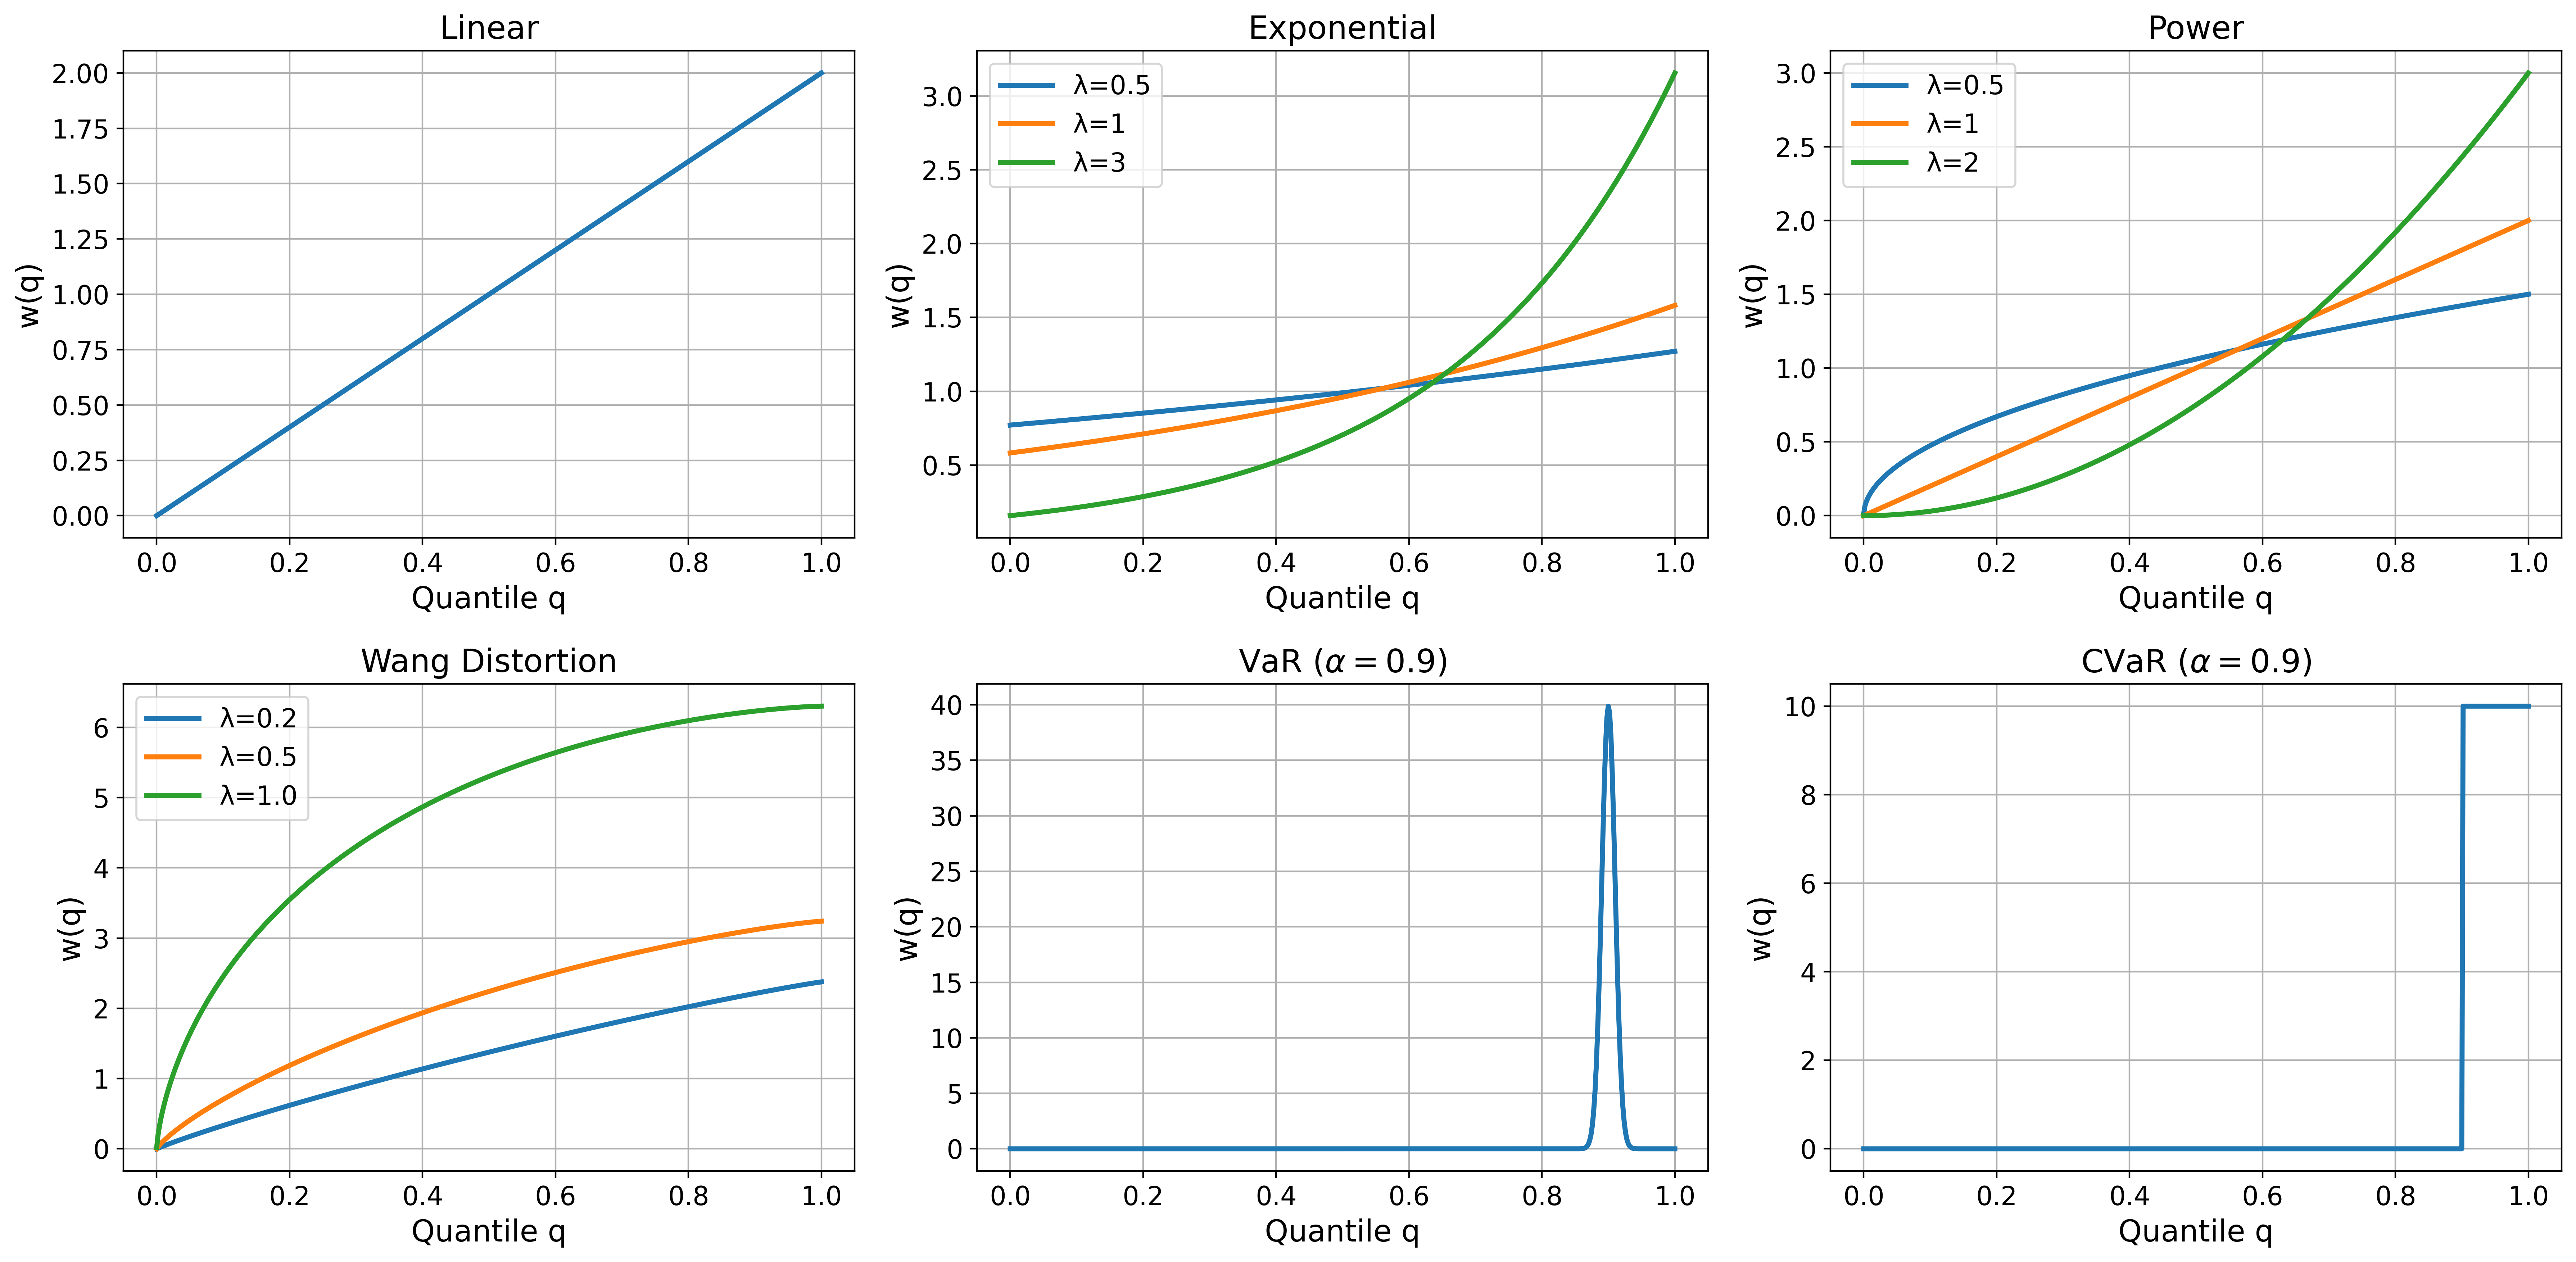
\includegraphics[width=0.9\textwidth]{figs/spectral_weights_comparison.png}
  \caption{Illustration of spectral weighting functions corresponding to different spectral risk measures (SRMs). For parameterized families, the plots show how the spectral weights vary with the risk-aversion parameter $\lambda$. Note that VaR is represented as a gaussian with very small bandwidth instead of a dirac delta for implementation reasons. \yc{add the params used for wang in the plot} } 
  \label{fig:srm-illustration}
\end{figure}

% \aj{-------------------------------}

% This appendix derives the RAD policy-gradient estimator in Theorem~\ref{thm:sard_pg}.
% We decompose the gradient of the FSD term into (i) a \emph{particle gradient} (sensitivity of the FSD loss to quantile-particle locations) and (ii) a \emph{quantile gradient} (sensitivity of those quantile locations to $\theta$), and then combine them.

% \subsection{Quantile-particle approximation of the cost distribution}
% For each policy $\pi$, define the induced cost random variable $C(\pi):=c_\psi(x,y)$ with $x\sim D_x$ and $y\sim\pi(\cdot\mid x)$.
% Fix quantile levels $\alpha_1<\dots<\alpha_N$ in $(0,1)$ and define the corresponding quantile values
% $q_i(\pi):=Q_{C(\pi)}(\alpha_i)$.
% We approximate the cost distribution of $\pi$ by the empirical measure in \emph{quantile-value space}
% \[
%   \hat\mu_\pi \;:=\;\frac1N\sum_{i=1}^N \delta_{q_i(\pi)}.
% \]
% In practice, $q_i(\pi)$ is computed from samples of $C(\pi)$ by empirical quantiles.

% \subsection{Chain-rule decomposition}
% Using the approximation $L_{\mathrm{FSD}}\big(C(\pi_\theta),C(\pi_{\mathrm{ref}})\big)\approx
% L_{\mathrm{FSD}}\big(\hat\mu_{\pi_\theta},\hat\mu_{\pi_{\mathrm{ref}}}\big)$, we write
% \begin{align}
%   \nabla_\theta L_{\mathrm{FSD}}\!\big(\hat\mu_{\pi_\theta},\hat\mu_{\pi_{\mathrm{ref}}}\big)
%   &=
%   \nabla_\theta L_{\mathrm{FSD}}\!\Big(\{q_i(\pi_\theta)\}_{i=1}^N,\{q_i(\pi_{\mathrm{ref}})\}_{i=1}^N\Big) \\
%   &=
%   \sum_{i=1}^N \frac{\partial L_{\mathrm{FSD}}}{\partial q_i(\pi_\theta)}\,\nabla_\theta q_i(\pi_\theta).
% \end{align}
% % which matches the decomposition used in the main draft (Eqs.~(14)--(15)).

% \subsection{Particle gradient via entropic OT and Sinkhorn}
% The unregularized OT formulation of $L_{\mathrm{FSD}}$ with cost $c(x,y)=(y-x)_+$ is generally non-smooth in particle locations.
% We therefore compute particle gradients through the entropically-regularized OT objective
% \[
%   L_{\mathrm{FSD}}^\varepsilon(\hat\mu_{\pi_\theta},\hat\mu_{\pi_{\mathrm{ref}}})
%   :=\mathrm{OT}^{\varepsilon}_{(y-x)_+}(\hat\mu_{\pi_\theta},\hat\mu_{\pi_{\mathrm{ref}}}),
% \]
% whose optimizer admits the Sinkhorn scaling form and is differentiable with respect to particle locations.
% In implementation we run a fixed number of Sinkhorn iterations and backpropagate to obtain
% $\frac{\partial L_{\mathrm{FSD}}}{\partial q_i(\pi_\theta)}$.

% \subsection{Quantile gradient via implicit differentiation and REINFORCE}
% Each quantile value $q_i(\pi_\theta)$ satisfies the defining equation
% \[
%   F_\theta\big(q_i(\pi_\theta)\big)=\alpha_i,
%   \qquad
%   F_\theta(t):=\mathbb{P}\big(C(\pi_\theta)\le t\big).
% \]
% Differentiating w.r.t.\ $\theta$ yields (by the implicit function theorem) the identity
% \[
%   \nabla_\theta q_i(\pi_\theta)
%   =
%   -\frac{\nabla_\theta F_\theta(t)\vert_{t=q_i(\pi_\theta)}}{f_\theta\big(q_i(\pi_\theta)\big)},
% \]
% where $f_\theta$ is the density of $C(\pi_\theta)$ at the quantile (when it exists).
% Estimating $f_\theta$ can be nontrivial; following the main draft, one may absorb $1/f_\theta$ into the step-size or use a density estimate, which leads to the approximation recorded in Eq.~(16) of the draft.

% Next, we express $\nabla_\theta F_\theta(t)$ via the log-derivative trick:
% \begin{align}
%   \nabla_\theta F_\theta(t)
%   &=\nabla_\theta \mathbb{E}_{x\sim D_x,\,y\sim\pi_\theta(\cdot\mid x)}\!\big[\mathbf{1}(c_\psi(x,y)\le t)\big]\\
%   &=
%   \mathbb{E}_{x\sim D_x,\,y\sim\pi_\theta(\cdot\mid x)}\!\big[\mathbf{1}(c_\psi(x,y)\le t)\,\nabla_\theta\log\pi_\theta(y\mid x)\big].
% \end{align}
% Substituting $t=q_i(\pi_\theta)$ and combining with the chain rule gives
% \[
%   \nabla_\theta L_{\mathrm{FSD}}\!\big(\hat\mu_{\pi_\theta},\hat\mu_{\pi_{\mathrm{ref}}}\big)
%   =
%   \mathbb{E}_{x,y}\Bigg[
%     \Bigg(\sum_{i=1}^N
%       \Big(-\frac{\partial L_{\mathrm{FSD}}}{\partial q_i(\pi_\theta)}\Big)\,
%       \mathbf{1}(c_\psi(x,y)\le q_i(\pi_\theta))
%     \Bigg)\nabla_\theta\log\pi_\theta(y\mid x)
%   \Bigg],
% \]
% (up to the density factor discussed above).

% \subsection{Completion of the proof of Theorem~\ref{thm:sard_pg}}
% Finally, since
% $L(\theta,\lambda)=\mathbb{E}[\tilde r(x,y)] + \lambda(L_{\mathrm{FSD}}-\kappa)$,
% adding the standard REINFORCE gradient for $\mathbb{E}[\tilde r(x,y)]$ and grouping terms yields Eq.~\eqref{eq:sard_pg}.
% The weighted case follows identically by inserting weights $w(\alpha_i)$ in the Riemann-sum approximation of $L_{\mathrm{FSD}}^{w}$.
% \qed

% Content that appears after the references are not part of the ``main text,'' have no page limits, are not necessarily reviewed, and should not contain any claims or material central to the paper.
% %
% If your paper includes supplementary materials, use the
% \begin{center}
%   {\tt {\textbackslash}beginSupplementaryMaterials}
% \end{center}
% command as in this example, which produces the title and disclaimer above.
% %
% If your paper does not include supplementary materials, this command can be removed or commented out.

\end{document}
